\documentclass{report}

% Language setting
% Replace `english' with e.g. `spanish' to change the document language
\usepackage[english]{babel}

% Set page size and margins
% Replace `letterpaper' with `a4paper' for UK/EU standard size
\usepackage[letterpaper,top=2cm,bottom=2cm,left=3cm,right=3cm,marginparwidth=1.75cm]{geometry}

% Useful packages
\usepackage{amsmath}
\usepackage{graphicx}
\usepackage[colorlinks=true, allcolors=blue]{hyperref}
\usepackage[style=ieee, backend=biber]{biblatex}
\addbibresource{bibliography.bib}
\usepackage{csquotes}
\usepackage{float}
\usepackage{listings}
\usepackage{xcolor}

\definecolor{codegreen}{rgb}{0,0.6,0}
\definecolor{codegray}{rgb}{0.5,0.5,0.5}
\definecolor{codepurple}{rgb}{0.58,0,0.82}
\definecolor{backcolour}{rgb}{0.95,0.95,0.92}

\lstdefinestyle{mystyle}{
    backgroundcolor=\color{backcolour},   
    commentstyle=\color{codegreen},
    keywordstyle=\color{magenta},
    numberstyle=\tiny\color{codegray},
    stringstyle=\color{codepurple},
    basicstyle=\ttfamily\footnotesize,
    breakatwhitespace=false,         
    breaklines=true,                 
    captionpos=b,                    
    keepspaces=true,                 
    numbers=left,                    
    numbersep=5pt,                  
    showspaces=false,                
    showstringspaces=false,
    showtabs=false,                  
    tabsize=2
}
\lstset{style=mystyle}


\title{High Performance Computing Project - A.A. 2022/2023}
\author{Andres Bermeo Marinelli}

\begin{document}
\maketitle
\tableofcontents
\chapter{Benchmarking MKL, OpenBLAS, and BLIS}

\section{Introduction}

In this exercise we compare the performance of three High Performance Libraries
(HPC): MKL, OpenBLAS, and BLIS. In particular, we focus on the level 3 BLAS 
function called \texttt{gemm}, which multiples an $m \times k$ matrix $A$ times 
a $k \times n$ matrix $B$ and stores the result in an $m \times n$ matrix $C$. 

This function comes in two types, one for single 
precision (float) and the other for double precision (double). Furthermore, it 
is capable of exploiting paralellism using OpenMP (OMP) to speed up the 
calculations, provided that we have the required computational resources.

Using squared matrices only, we perform a scalability study in two scenarios. 
In the first scenario, we fix the number of cores, and increase the size of the
matrices from $2000$ to $20000$. In the second scenario, we fix the matrix size 
to $10000$ and increase the number of cores that \texttt{gemm} can use by 
modifying the \texttt{OMP\_NUM\_THREADS} environment variable.

In both scenarios, we repeat the measurements for both single and double
precision, for both THIN and EPYC nodes, using the maximum number of cores.

Furthermore, for the second scenario, we also modify the thread affinity policy 
of OMP in order to observe any differences.

\section{Methodology}

\subsection{Compiling BLIS and obtaining binaries}

We begin by downloading the BLIS library by using the following commands:
\begin{lstlisting}[language=bash]
    $git clone https://github.com/flame/blis.git
    $cd blis
    $srun -p {NODE} -n1 ./configure --enable-cblas --enable-threading=openmp \
    \ --prefix=/path/to/myblis/lib auto
    $srun -p {NODE} -n 1 --cpus-per-task={P} make -j {P}
    $make install
\end{lstlisting}

Where \texttt{NODE} can be specified as either \texttt{THIN} or \texttt{EPYC} and 
\texttt{P} are the available cores for each node, $24$ and $128$ respectively.

With these commands, we have compiled the BLIS library for the desired 
architecture.

Next, we specify the flag in the Makefile to compile for float or double using 
\texttt{\-DUSE\_FLOAT} or \texttt{\-DUSE\_DOUBLE}. Then, we run:
\begin{lstlisting}[language=bash]
    $salloc -n {P} -N1 -p {NODE} --time=1:0:0
    $module load mkl/latest
    $module load openBLAS/0.3.23-omp
    $export LD_LIBRARY_PATH=/path/to/myblis/lib:$LD_LIBRARY_PATH
    $srun -n1 make cpu
\end{lstlisting}

Which will generate the binaries for the desired architecture, with floar or 
double precision, depending on the flag we used.

To run, we use: 
\begin{lstlisting}[language=bash]
    $srun -n1 --cpus-per-task=128  ./gemm_mkl.x {size_M} {size_K} {size_N}
    $srun -n1 --cpus-per-task=128  ./gemm_oblas.x {size_M} {size_K} {size_N}
    $srun -n1 --cpus-per-task=128  ./gemm_blis.x {size_M} {size_K} {size_N}
\end{lstlisting}

At the end of this procedure, we should have the appropriate binaries for each 
architecture, and for each type of precision, double or float.

We now detail the steps to obtain the measurements for both scenarios.

\subsection{Using a fixed number of cores}

For this section, we use all the cores available in a THIN or an EPYC node: 24 
and 128, respectively. 

Since we only use squared matrices, we can describe the dimensions of the matrices 
with a single number, which we call "size". 

For both architectures, we start with a size of $2000$ and end with a size of 
$20000$, with jumps of $2000$ for a total of $10$ sizes. For each size, 
we repeat the measurement $10$ times and report the average and standard 
deviation.

Finally, we repeat the measurements for both floating point precision and double 
point precision.

The scripts that were used can be found in the folder \texttt{exercise2/scripts}, 
under the name \texttt{es2\_1\_thin.sh} and \texttt{es2\_1\_epyc.sh}.

It is important to observe that in this section, since we are using the entire 
node, there is little possibility to play with combinations of thread affinity.

This will be done for the next section.

Furthermore, contrary to the guidelines for the exercise, we decided to use the 
entire node to benchmark its full capacity, and also to avoid wasting 
resources. 

In fact, to obtain an accurate benchmark, we need to reserve the whole node, 
regardless of the number of cores we decide to use. This is because if other 
people began to use the other half of the node, this could introduce additional 
workloads which interfere with the benchmark. 

\subsection{Using a fixed matrix size}

For this section, we fix the size of the matrices to $10000$. Then, we slowly 
increase the number of cores to be used, until we reach the maximum. 

To set the number of cores, we change the environment variable 
\texttt{OMP\_NUM\_THREADS} to the desired value.

For THIN nodes, which have $24$ cores, we start using $1$ core, then $2$ and 
then we increase by steps of $2$, for a total of 13 points.

For EPYC nodes, which have $128$ cores, we start from $1$, then $10$ and then 
we increase by steps of $10$ until $120$. We also use $128$ cores, to see what 
happens at full capacity. We obtain a total of $14$ points.

We repeat all measurements $10$ times and report the average and standard 
deviation.

As usual, we repeat this process for both floating and double point precision.

In this section, we have the liberty to explore different thread allocation 
policies since we are not always using the whole node. 

We decided to use following combinations:
\begin{enumerate}
    \item \texttt{OMP\_PLACES=cores} and \texttt{OMP\_PROC\_BIND=close} 
    \item \texttt{OMP\_PLACES=cores} and \texttt{OMP\_PROC\_BIND=spread} 
\end{enumerate}

The scripts that were used can be found in the folder \texttt{exercise2/scripts}, 
under the names \texttt{es2\_2\_close\_thin.sh}, \texttt{es2\_2\_close\_epyc.sh}, 
\texttt{es2\_2\_spread\_thin.sh}, and \texttt{es2\_2\_spread\_epyc.sh}.

\section{Results and Discussion}

Before we discuss the results of both exercises individually, we briefly 
introduce the equation to calculate the theoretical peak performance ($T_{pp}$) 
of a machine:

\begin{equation}\label{eq:perf}
    T_{pp} = \text{Core Count}\times \text{clock freq.} \times \text{IPC}
\end{equation}

Where \texttt{IPC} is the instructions per cycle that the architecture 
is capable of executing.

This equation is very intuitive. The clock frequency tells us how many cycles 
per second a single core is able to achieve. The ipc factor tells us how many 
instructions per cycle the core can execute. This number is different for 
single precision (SP) and double precision (DP) operations. Finally, we need 
to multiple this by the number of cores that our machine has. 

On orfeo, THIN and EPYC nodes are composed of: 
\begin{itemize}
    \item THIN: $24$ Intel(R) Xeon(R) Gold $6126$ CPU's at $2.60$GHz - Skylake
    \item EPYC: $128$ EPYC AMD 7H12 CPU's at $2.60$GHz - Zen 2 (7002 a.k.a "Rome")
\end{itemize}

Skylake architecture is reported\cite{arch} to be able to execute $64$ SP FLOP per cycle 
and $32$ DP FLOP per cycle. On the other hand, Zen 2 is reported\cite{arch} to execute 
$32$ SP FLOP per cycle and $16$ DP FLOP per cycle.

Therefore, we obtain: 

\begin{table}[H]
\centering
\begin{tabular}{|c|c|c|c|c|c|}
    \hline
    Node Type & Total Cores & IPC (SP) & IPC (DP) & $T_{pp}$ (SP) & $T_{pp}$ (DP)\\\hline
    THIN      &     24      &    64    &   32     & $\sim 4$ TFLOPS & $\sim 2$ TFLOPS \\
    EPYC      &    128      &    32    &   16     & $\sim 10.6$ TFLOPS & $\sim 5.3$ TFLOPS \\ \hline
\end{tabular}
\caption{\label{tab:perf}Performance table of THIN and EPYC node architectures.}
\end{table}

Now we can proceed to discuss the results of the exercise.

\subsection{Using a fixed number of cores}

As mentioned above, in this section we keep the number of cores fixed to the 
maximum available in the node, namely 24 for THIN and 128 for EPYC, and we 
slowly increase the size of the matrices being multiplied from $m=2000$ to 
$m=20000$. 

We first show the results for THIN and then for EPYC nodes.

\subsubsection{THIN Nodes}

\begin{figure}[H]
% \centering
\hspace*{-2.5cm}
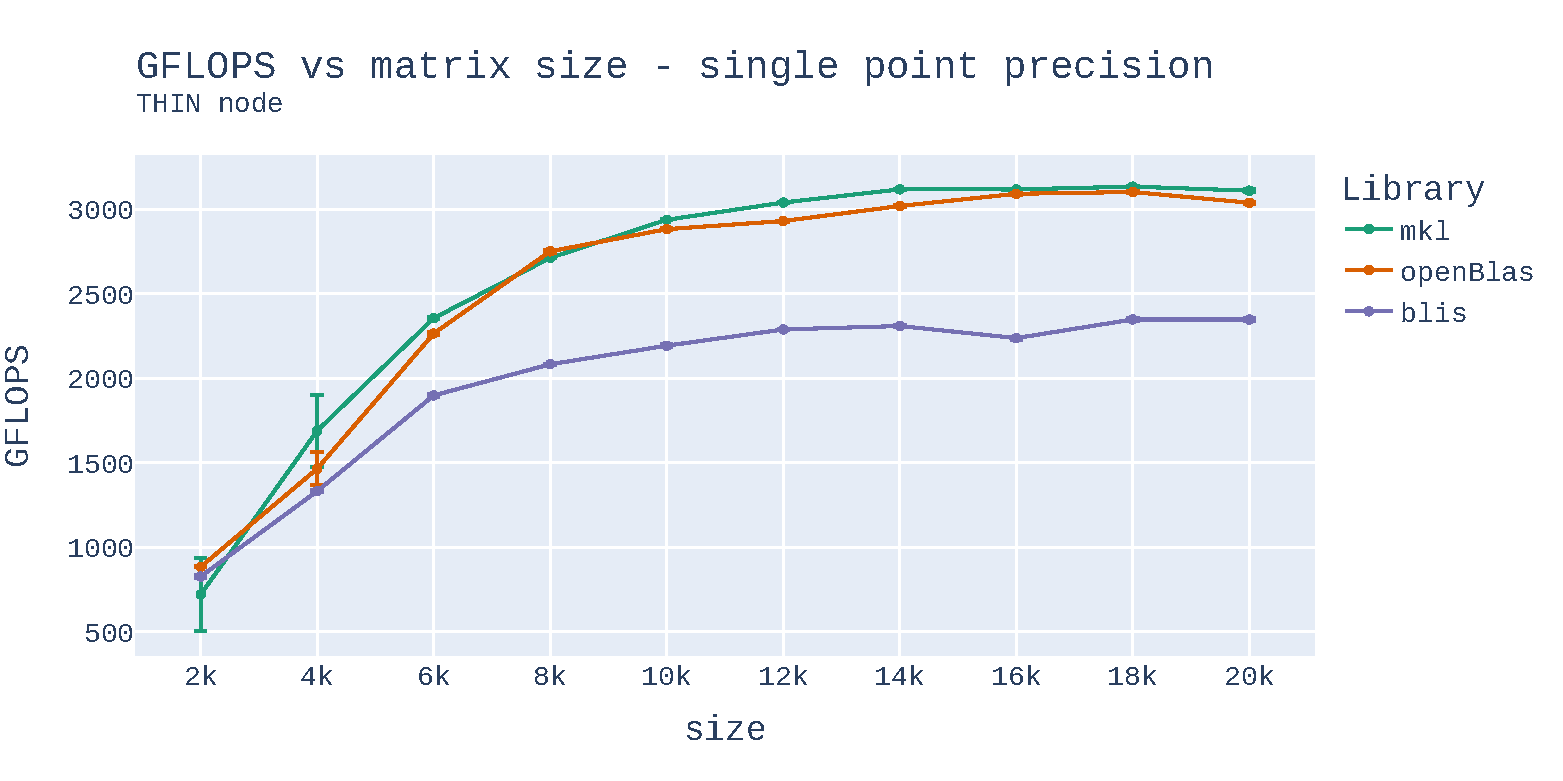
\includegraphics[width=10cm, height=6cm]{./images/fixed_cores_thin_float_gflops.pdf}
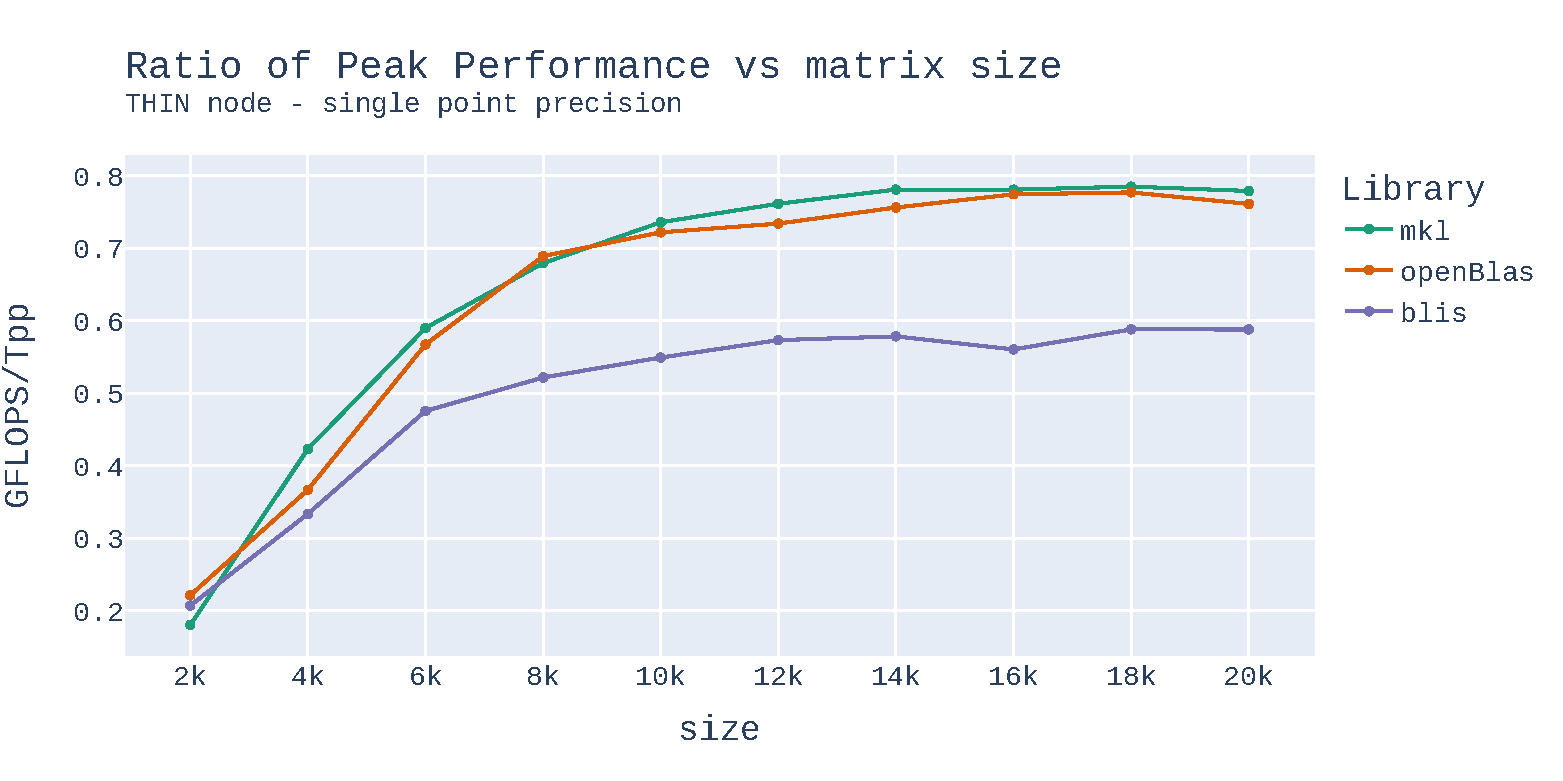
\includegraphics[width=10cm, height=6cm]{./images/fixed_cores_thin_float_gflops_ratio.pdf}
\caption{\label{fig:fixed_cores_thin_float} Results of SP matrix-matrix multiplication 
for THIN nodes. \texttt{MKL} and \texttt{OpenBLAS} perform similarly, outperforming 
\texttt{BLIS} for all matrix sizes.}
\end{figure}

We see that both \texttt{MKL} and \texttt{OpenBLAS} are able to reach $\sim 3.2$ 
TFLOPS, which is around $\sim80\%$ of $T_{pp}$. On the other hand, the \texttt{BLIS}
library is not able to exploit the full potential of the machine, arriving only
to $\sim 2.4$ TFLOPS, which is $\sim60\%$ of $T_{pp}$.

Furthermore, looking at the ratio of peak performance on the right, we observe 
that for small matrix sizes, none of the libraries are able to fully exploit 
the theoretical peak performance of the machine. This is most likely because the 
problem size is so small, that the majority of cores are starving for data rather 
than crunching numbers. In fact, we are able to reach the best performance when 
dealing with matrices of size $20000$. 

\begin{figure}[H]
% \centering
\hspace*{-2.5cm}
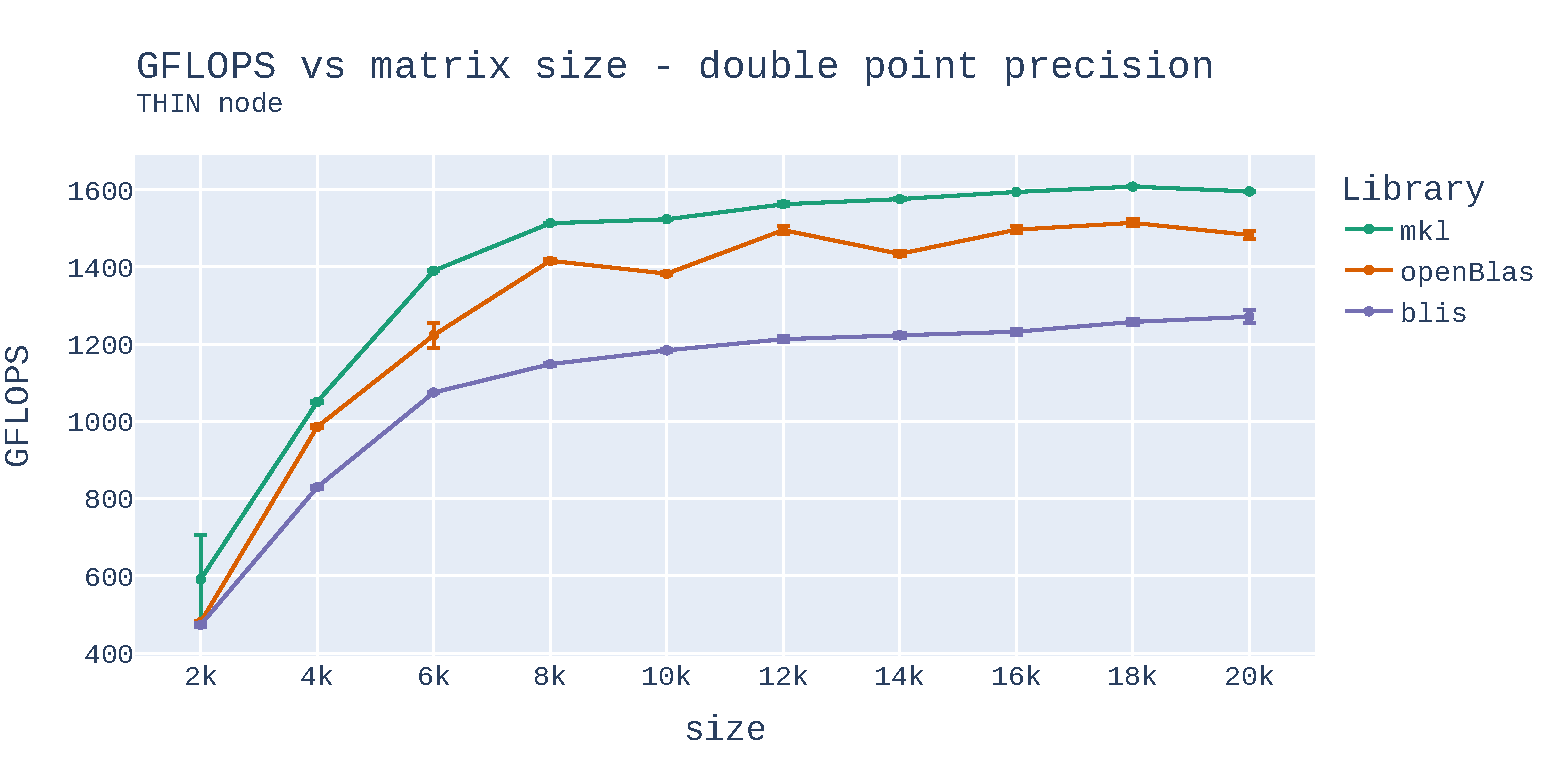
\includegraphics[width=10cm, height=6cm]{./images/fixed_cores_thin_double_gflops.pdf}
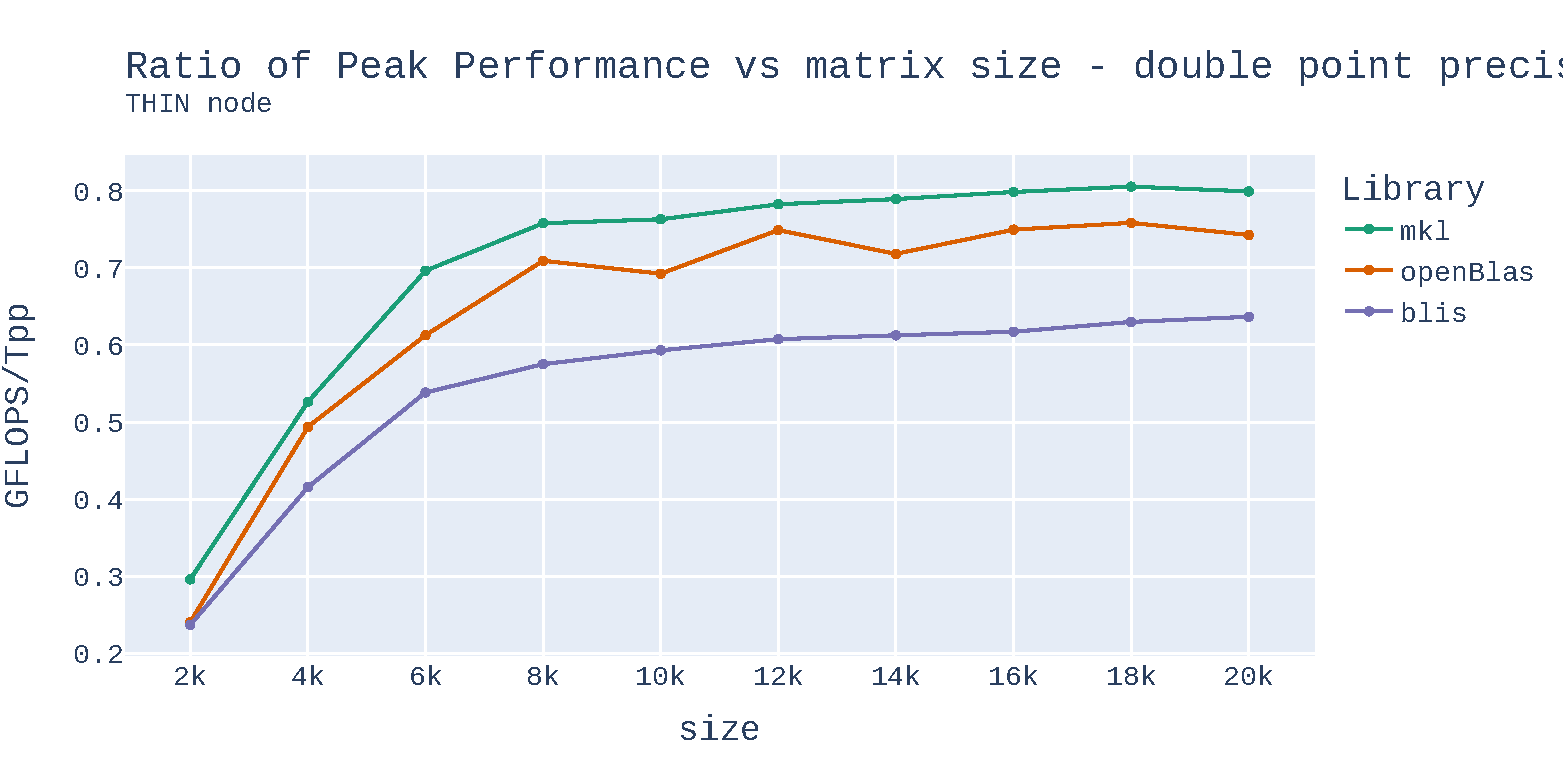
\includegraphics[width=10cm, height=6cm]{./images/fixed_cores_thin_double_gflops_ratio.pdf}
\caption{\label{fig:fixed_cores_thin_double} Results of DP matrix-matrix multiplication 
for THIN nodes. \texttt{MKL} performs the best, slightly above \texttt{OpenBLAS}. 
Both outperform \texttt{BLIS} for all matrix sizes.}
\end{figure}

We see that \texttt{MKL} reaches $\sim1.6$ TFLOPS, 
while \texttt{OpenBLAS} is slightly lower, at $\sim1.5$ TFLOPS, which is $\sim80\%$ and 
$\sim75\%$ of $T_{pp}$, respectively. On the other hand, \texttt{BLIS} arrives to 
$\sim1.3$ TFLOPS, which is $\sim65\%$ of $T_{pp}$.

Furthermore, since double precision is a heavier computation compared to single 
precision, we see that the libraries perform much better than the their single precision 
counterparts.
For example, looking at the plot for single precision, for matrix size of $4000$, 
we obtain on average around $40\%$ of $T_{pp}$. On the other hand, for double precision, 
looking at the same size, we are already at $50\%$ of $T_{pp}$.
\\

For both SP and DP, and for all matrix size, we notice that \texttt{MKL} and 
\texttt{OpenBLAS} are better able to exploit the full potential of a THIN node 
compared to \texttt{BLIS}. Therefore, on THIN nodes, if we need to multiply 
two matrices, we should always use either \texttt{MKL} or \texttt{OpenBLAS} to 
get some more performance. To get the absolute best performance, it is preferable 
to use \texttt{MKL}.

These results shouldn't be surprising, considering 
that \texttt{MKL} is developed by Intel and THIN nodes are Intel-based.
Therefore, it is natural to expect that this library is very fine-tuned to 
their own architecture and is able to exploit the performance of their machines.

Lastly, we observe the impressive results achieved by \texttt{OpenBLAS} which 
is based on the original implementation of Kazushige Goto, and is able to achieve a similar performance to 
\texttt{MKL}, which is maintained by an entire corporation.

\subsubsection{EPYC Nodes}

Now we show the results on EPYC nodes, which have a $T_{pp}$ of $10.6$ TFLOPS 
for SP and $5.3$ TFLOPS for DP.
\\\\
We first show the results of matrix-matrix multiplication for single point 
precision.

\begin{figure}[H]
% \centering
\hspace*{-2.5cm}
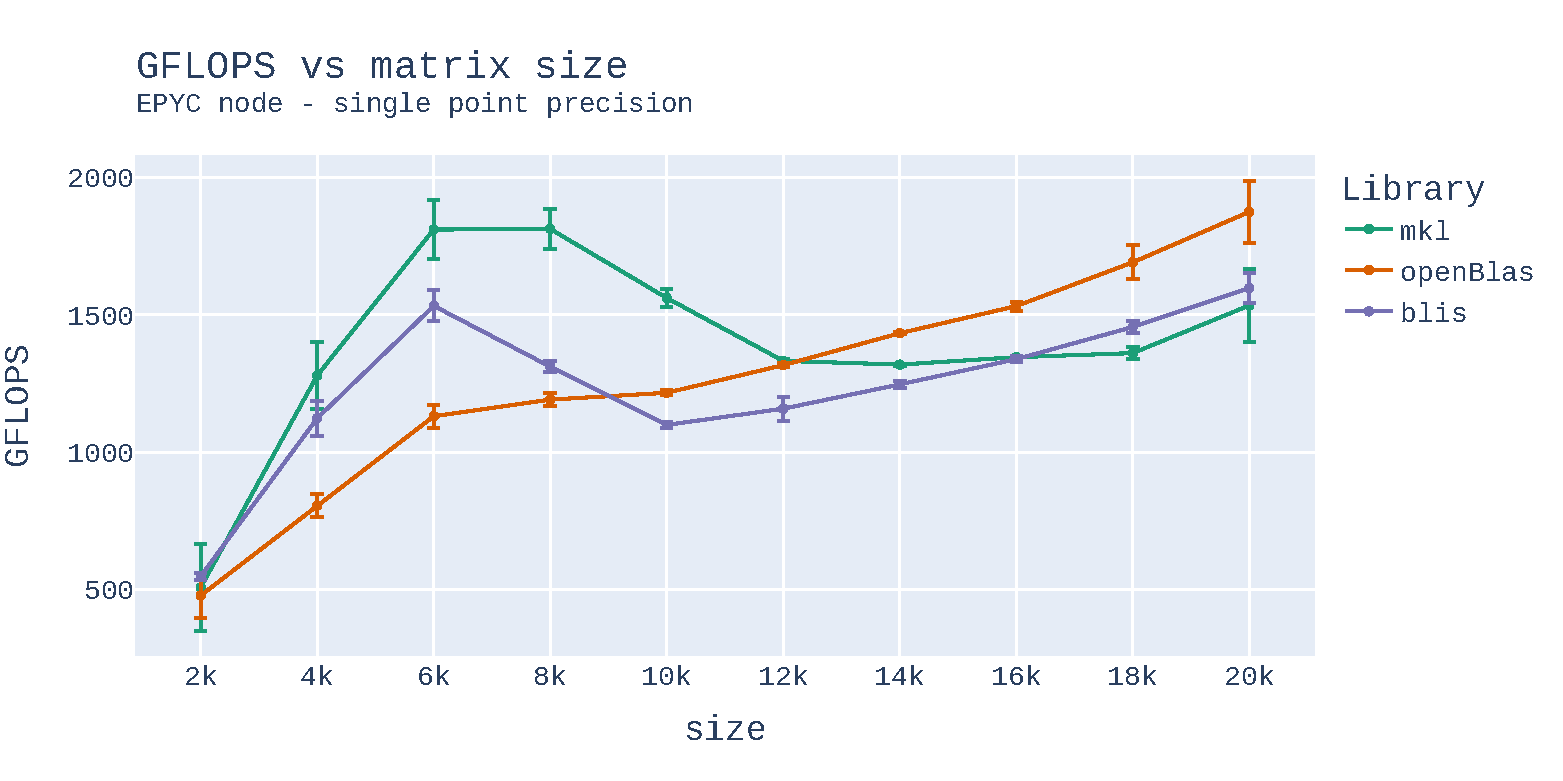
\includegraphics[width=10cm, height=6cm]{./images/fixed_cores_epyc_float_gflops.pdf}
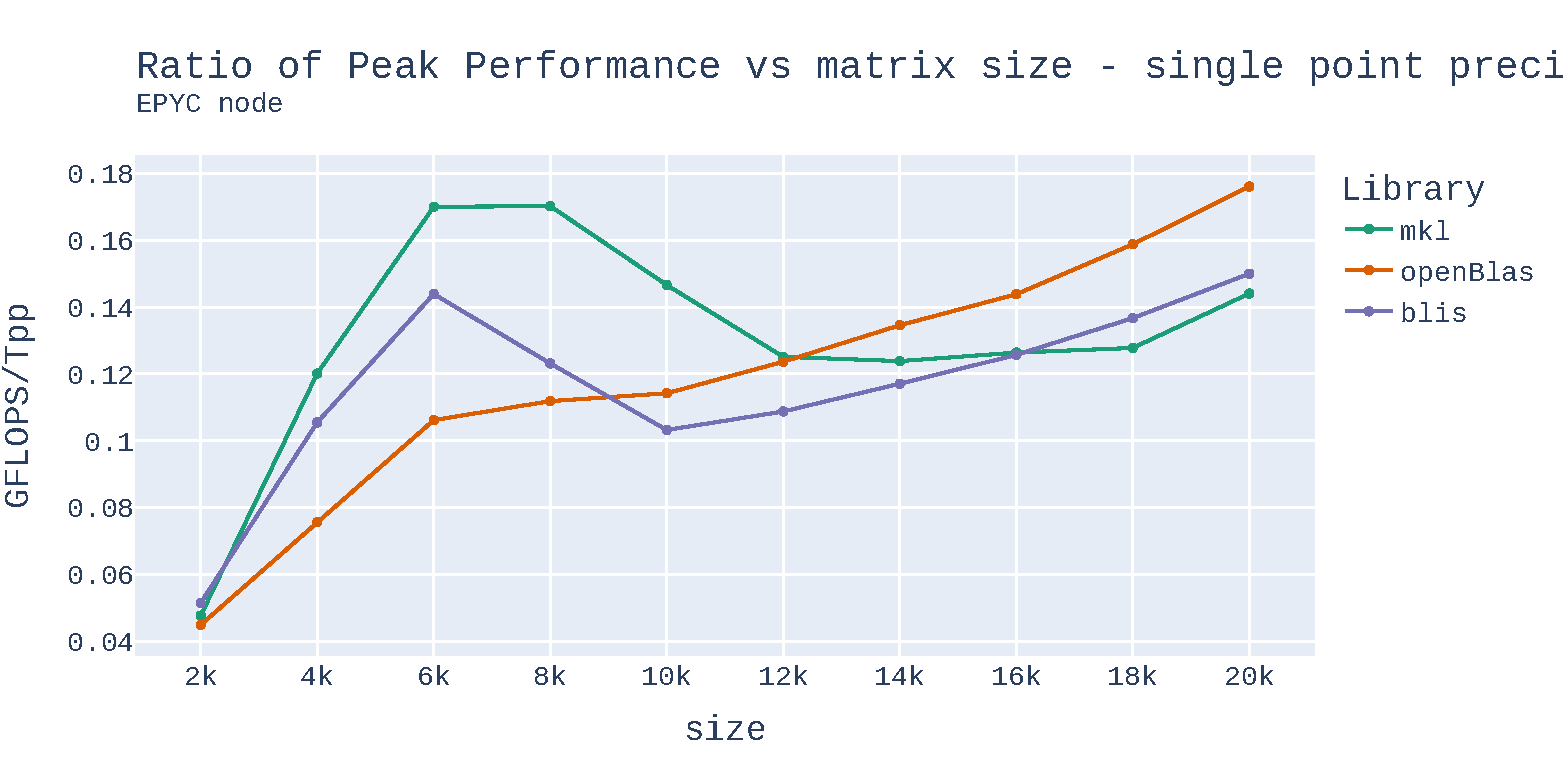
\includegraphics[width=10cm, height=6cm]{./images/fixed_cores_epyc_float_gflops_ratio.pdf}
\caption{\label{fig:fixed_cores_epyc_float} Results of SP matrix-matrix multiplication 
for EPYC nodes. We notice that asymptotically, \texttt{OpenBLAS} outperforms 
\texttt{MKL} and \texttt{BLIS}, while for small matrices, \texttt{OpenBLAS} 
performs the worst.}
\end{figure} 

In this case, none of the libraries are able to reach more than $18\%$ of $T_{pp}$.
This could be an indication that to properly exploit a full EPYC node, we need 
to multiply much bigger matrices.
\\

We also notice that for matrices of size $\leq 9000$, \texttt{MKL} and \texttt{BLIS} 
outperform \texttt{OpenBLAS}. Between sizes $9000$ and $12000$, \texttt{MKL} 
performs best and \texttt{OpenBLAS} begins outperform \texttt{BLIS}. 
For sizes $\geq 12000$, \texttt{OpenBLAS} performs the best.

\begin{figure}[H]
% \centering
\hspace*{-2.5cm}
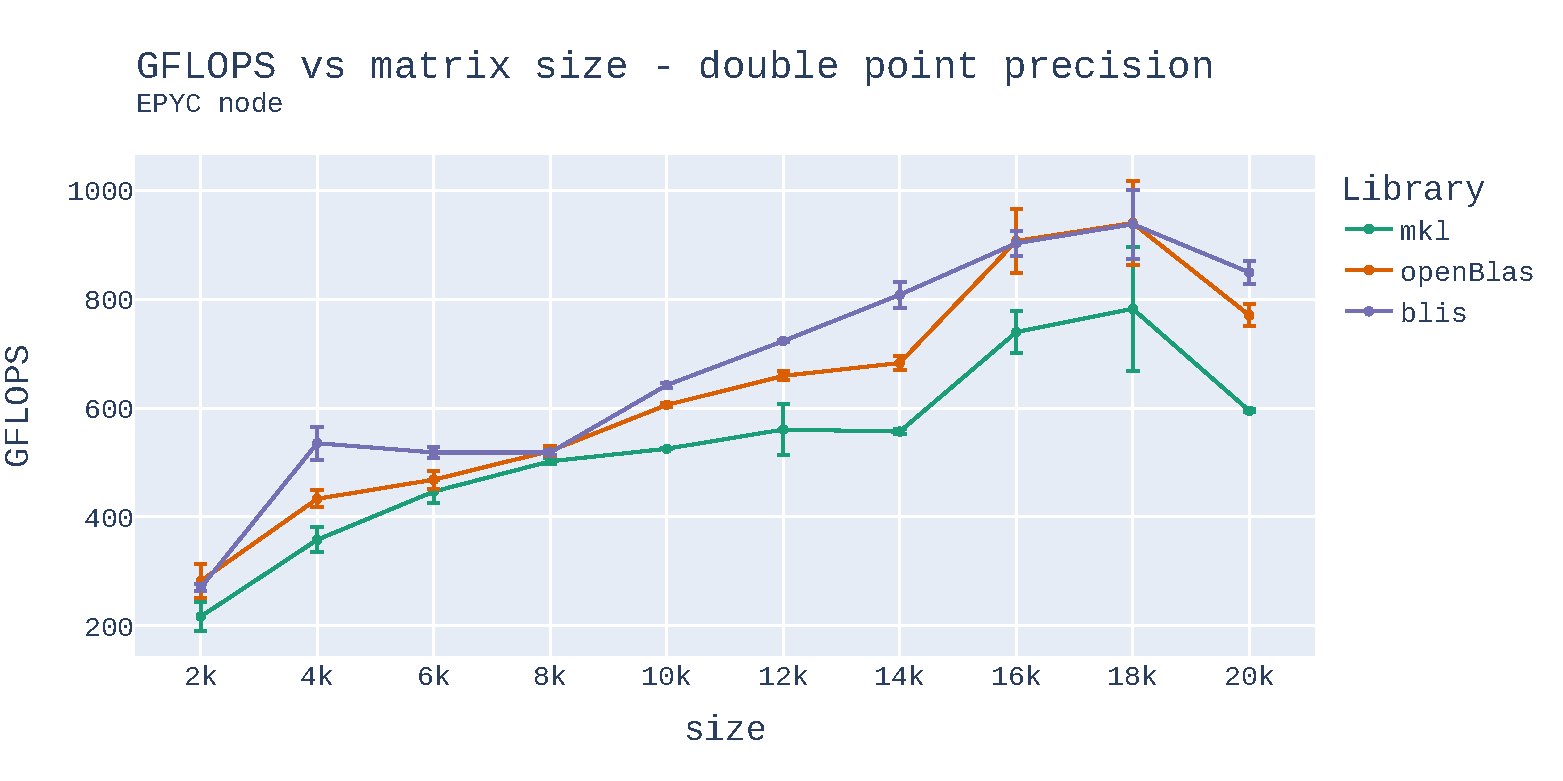
\includegraphics[width=10cm, height=6cm]{./images/fixed_cores_epyc_double_gflops.pdf}
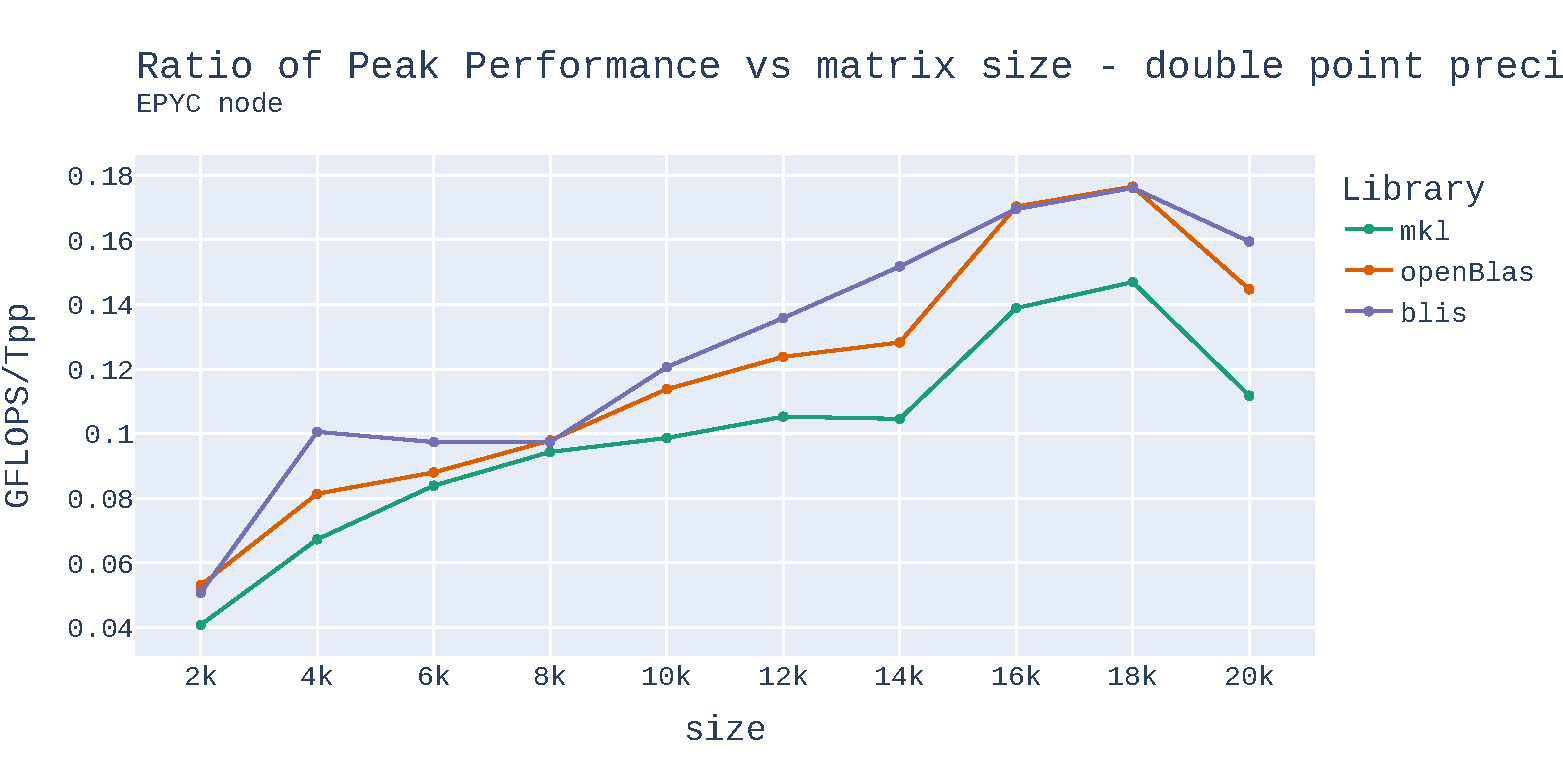
\includegraphics[width=10cm, height=6cm]{./images/fixed_cores_epyc_double_gflops_ratio.pdf}
\caption{\label{fig:fixed_cores_epyc_double} Results of DP matrix-matrix multiplication 
for EPYC nodes. \texttt{BLIS} outperforms \texttt{MKL} and \texttt{OpenBLAS} 
for all matrix sizes.}
\end{figure}

Again, we notice that none of the libraries are able to achieve more than $18\%$ 
of $T_{pp}$. However, in this case, \texttt{BLIS} outperforms the other two libraries 
for all matrix sizes. The next best performer is \texttt{OpenBLAS}, followed by 
\texttt{MKL}, which performs the worst.
\\

In conclusion, on EPYC nodes, it seems that for DP matrix-matrix multiplication, 
it is better to use \texttt{BLIS}, while for SP, it is very dependent on the 
size of the matrices. For large matrices, we should use \texttt{OpenBLAS}
while for smaller ones, we should use \texttt{MKL}. 
Furthermore, evidence suggests that to fully exploit and EPYC node, we need to 
deal with much bigger matrices. So if we are multiplying matrices of size up to 
$20000$, it is much more convenient to just use a THIN node to get more 
performance.

\subsection{Using a fixed matrix size}

In this section, we fix the matrix size to $10000$ and we slowly increase the 
amount of cores that the libraries can exploit for multithreading through OMP. 
For THIN nodes, we arrive to $24$ cores, while for EPYC nodes, we arrive to 
$128$ cores.

Furthermore, since we are slowly increasing the number of cores that the libraries 
can use for multithreading, we can study the effects of using different 
thread allocation policies. In particular, we chose to use 
\texttt{OMP\_PROC\_BIND=close} and \texttt{OMP\_PROC\_BIND=spread}, while 
always using \texttt{OMP\_PLACES=cores}. 

In the first case, the threads will slowly occupy first one entire socket, and 
then, when it is full, the other one. In the second case, the threads will be 
placed as spread apart as possible, most likely on different sockets. 
In both cases, when we use the full node, we expect the results to be the same.

Furthermore, in contrast to the previous part of the exercise, we compare the 
GFLOPS obtained with the $T_{pp}$ calculated with the cores that are being used. 
In other words, in equation\ref{eq:perf}, instead of using the full 24 or 128 
to calculate $T_{pp}$ for the whole node, we use the number of cores we are using 
for that calculation.

We first analyze THIN and then EPYC nodes.

\subsubsection{THIN Nodes}
\begin{figure}[H]
% \centering
\hspace*{-2.5cm}
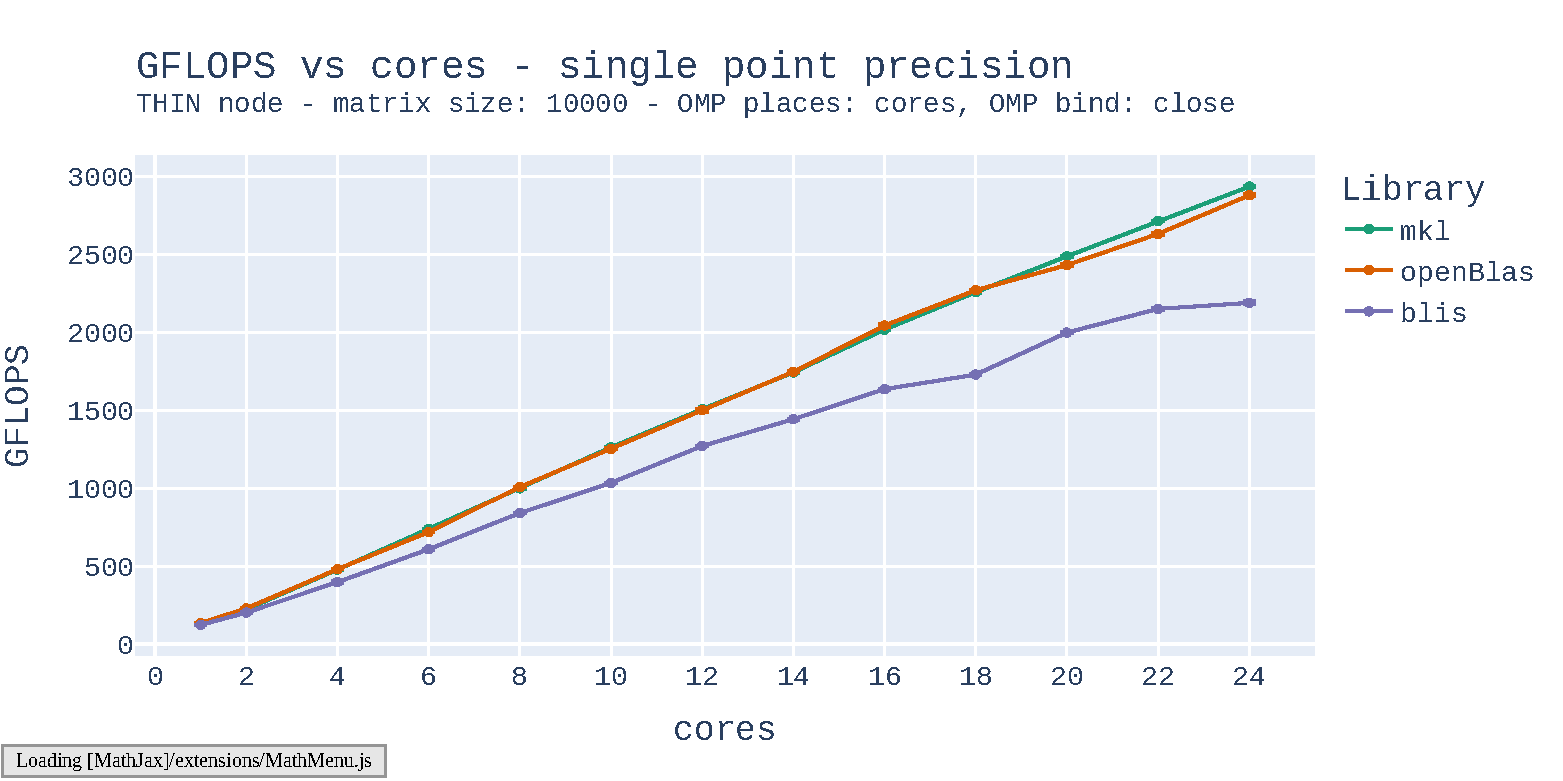
\includegraphics[width=10cm, height=6cm]{./images/fixed_size_thin_float_gflops_close.pdf}
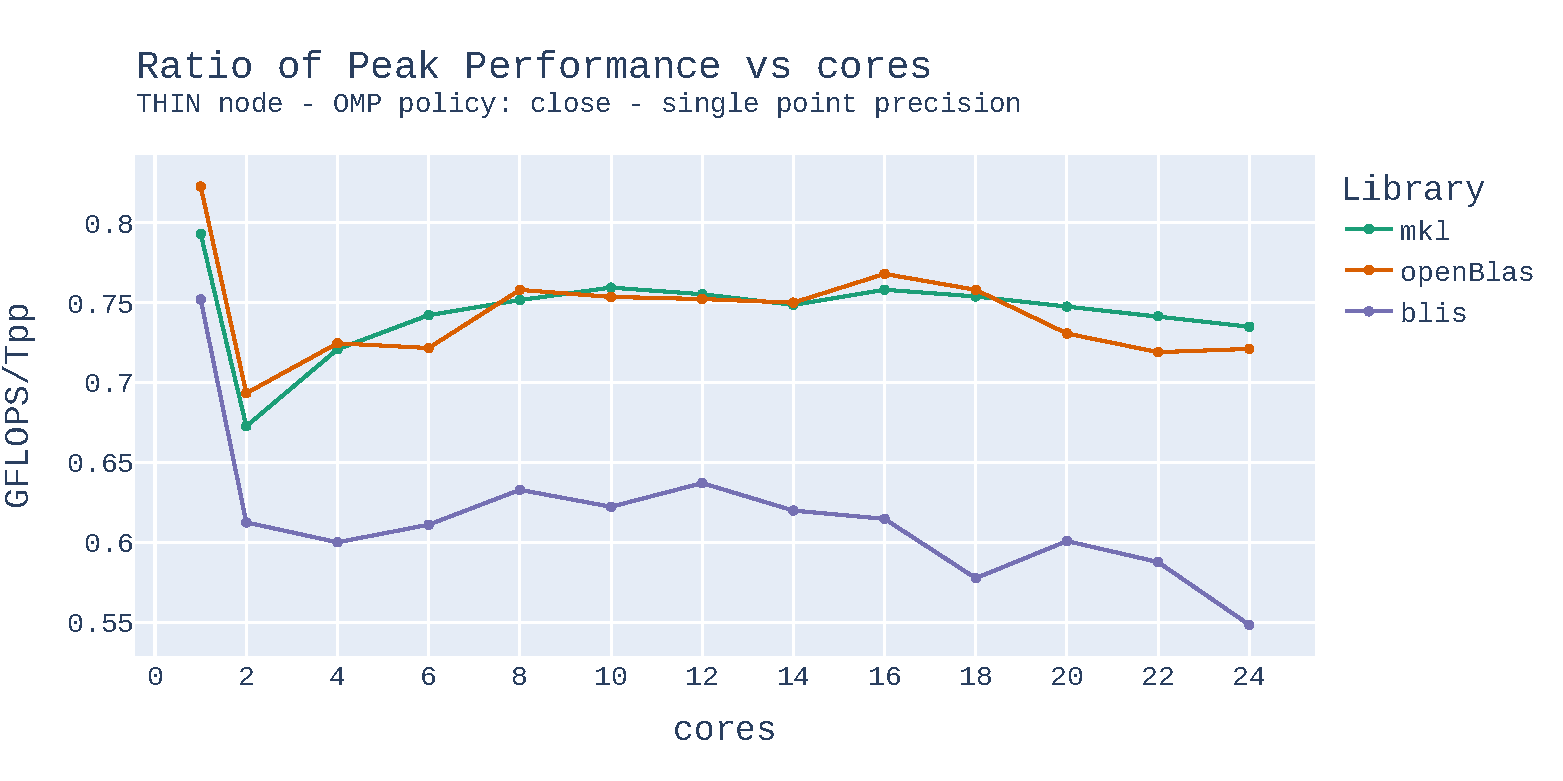
\includegraphics[width=10cm, height=6cm]{./images/fixed_size_thin_float_gflops_close_ratio.pdf}
\caption{\label{fig:fixed_size_thin_float_close} Results of SP matrix-matrix 
    multiplication as the number of cores increase, using OMP close policy. 
    \texttt{MKL} and \texttt{OpenBLAS} obtain the best performance.}
\end{figure}

As we can see from the graph, both \texttt{MKL} and \texttt{OpenBLAS} are able 
to maintain $\sim 75\%$ of $T_{pp}$ for cores $\geq 6$. On the other 
hand, \texttt{BLIS} is able to achieve $\sim 60\%$ of $T_{pp}$. With $24$ cores 
this figure decreases to $55\%$. 

Interestingly, we notice that with $2$ cores, there is a significant performance 
drop. This is most likely explained by the fact that both cores are mapped to the 
same socket due to the close policy and must share resources such as the higher 
level caches, causing some contention.

Furtermore, once again, we notice that the best performing library is 
\texttt{MKL} which is Intel-based, closely followed by \texttt{OpenBLAS}.
\\

Now we analyze the results using a spread policy.

\begin{figure}[H]
% \centering
\hspace*{-2.5cm}
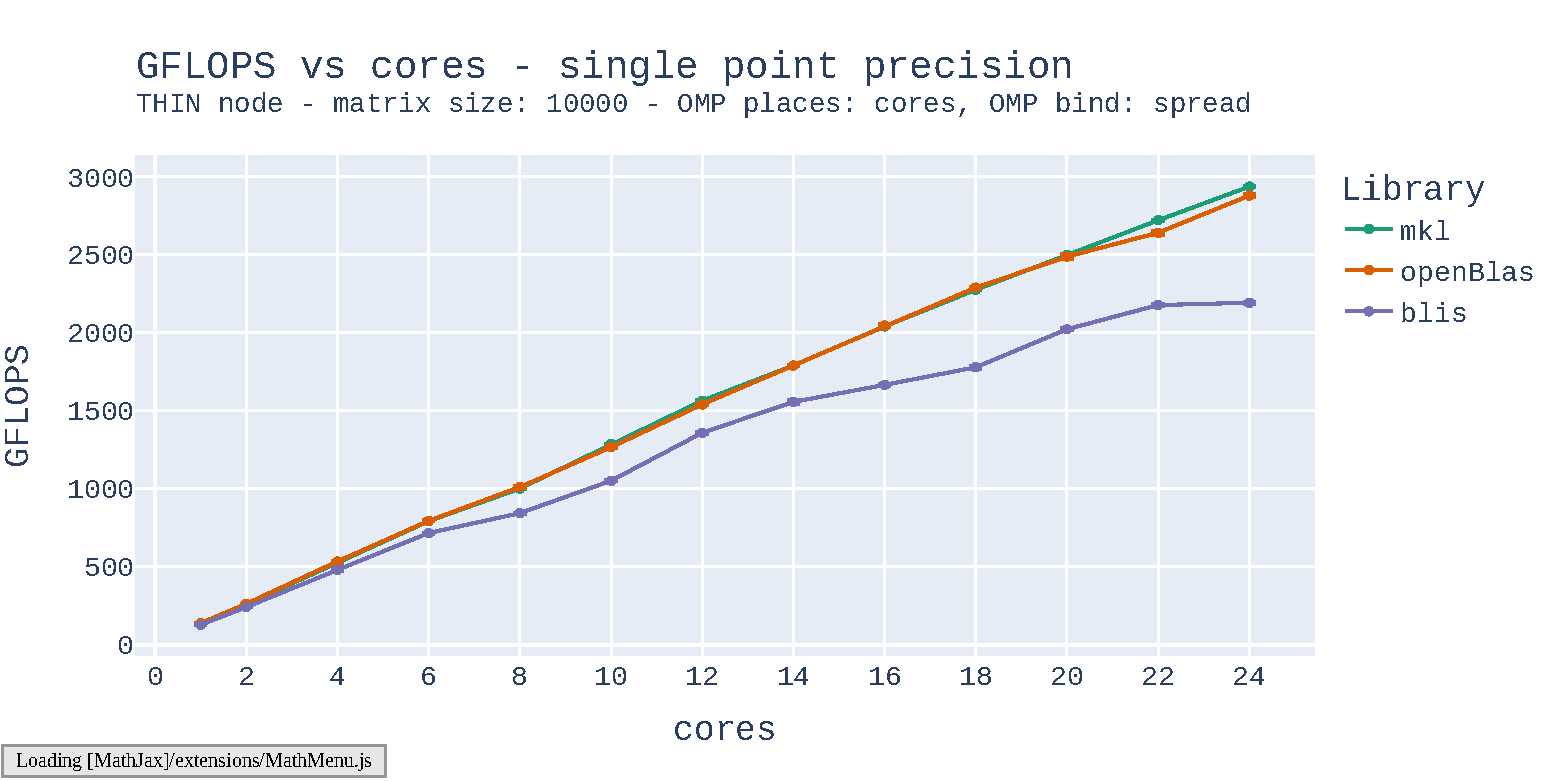
\includegraphics[width=10cm, height=6cm]{./images/fixed_size_thin_float_gflops_spread.pdf}
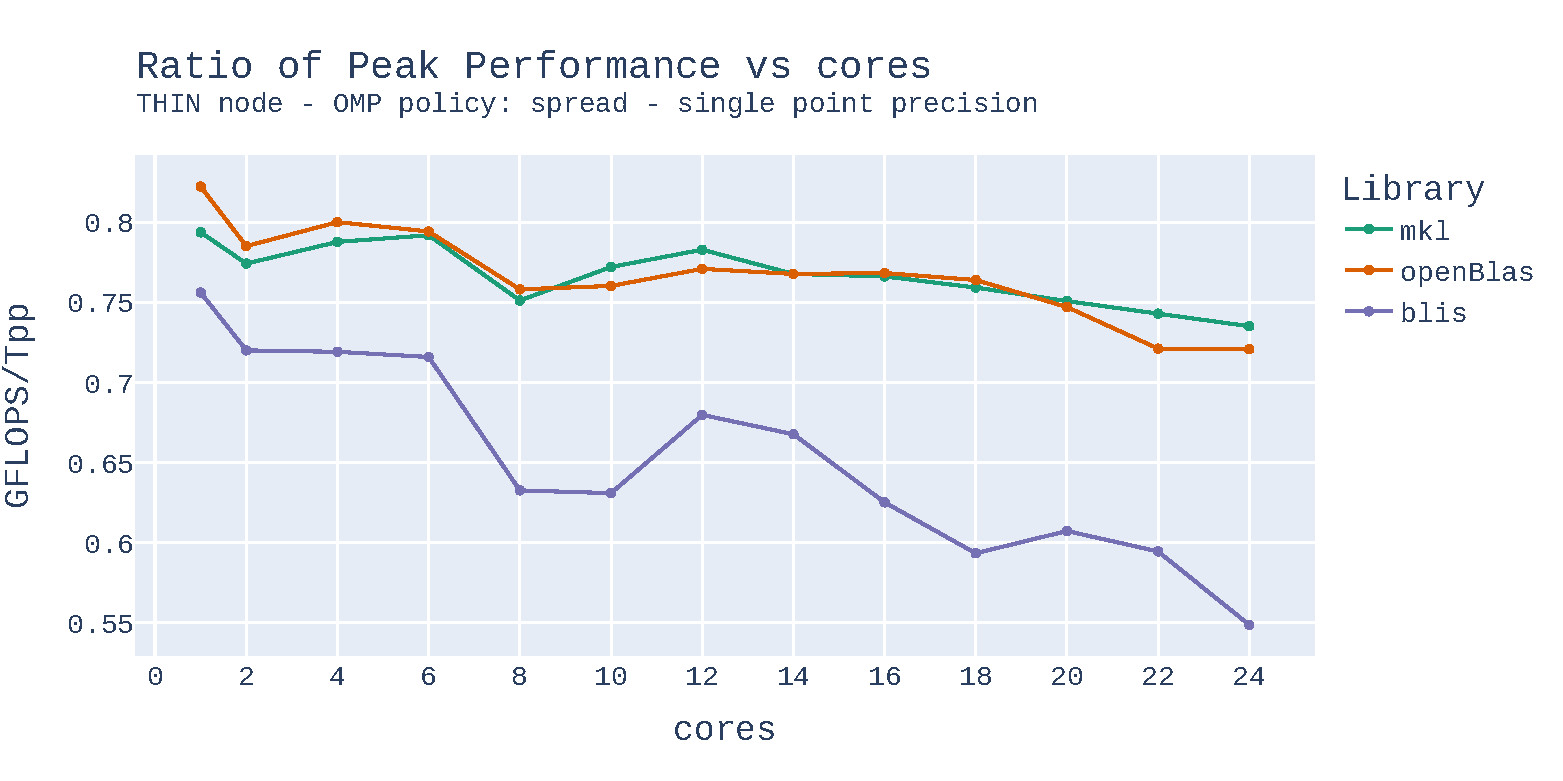
\includegraphics[width=10cm, height=6cm]{./images/fixed_size_thin_float_gflops_spread_ratio.pdf}
\caption{\label{fig:fixed_size_thin_float_spread} Results of SP matrix-matrix multiplication 
    as the number of cores increase, using OMP spread policy. \texttt{MKL} 
and \texttt{OpenBLAS} are the best perfomers.}
\end{figure}

Using a spread policy, we obtain very similar results to the case where we use 
a close policy. The main difference is that we don't have the same performance 
drop at 2 cores. This is most likely due to the fact that with a spread policy, 
each core is mapped to its own socket and there is no contention for resources. 

In fact, we notice that on average, the performance is slightly better than the 
close policy counterpart, and this is probably due to better resource usage 
from the beginning, since threads don't have to compete for resources immediately.
This highlights the importance of using the correct mapping policy to obtain 
better performance.
\\

Now we briefly analyze the results obtained for double precision.
\begin{figure}[H]
% \centering
\hspace*{-2.5cm}
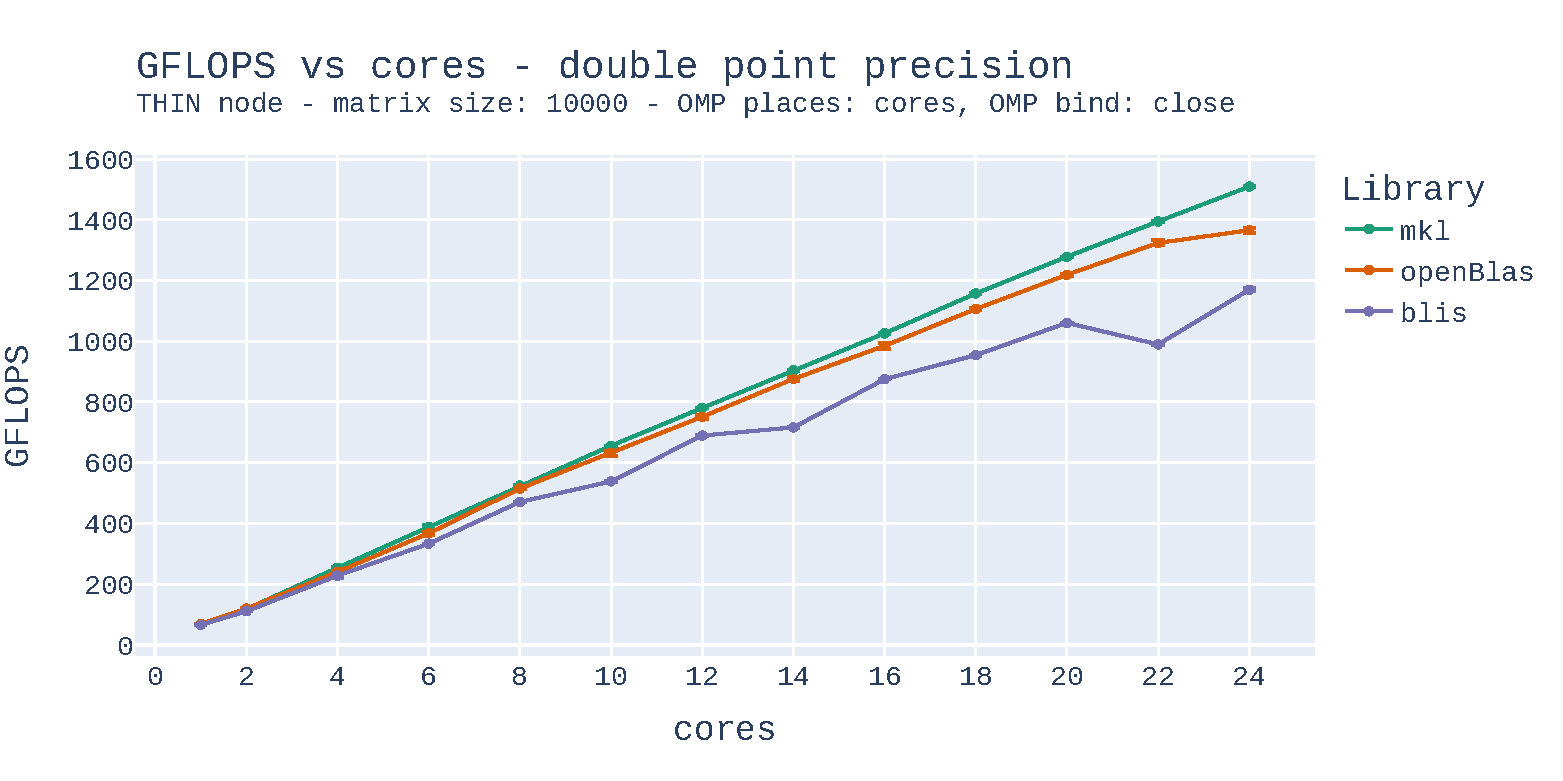
\includegraphics[width=10cm, height=6cm]{./images/fixed_size_thin_double_gflops_close.pdf}
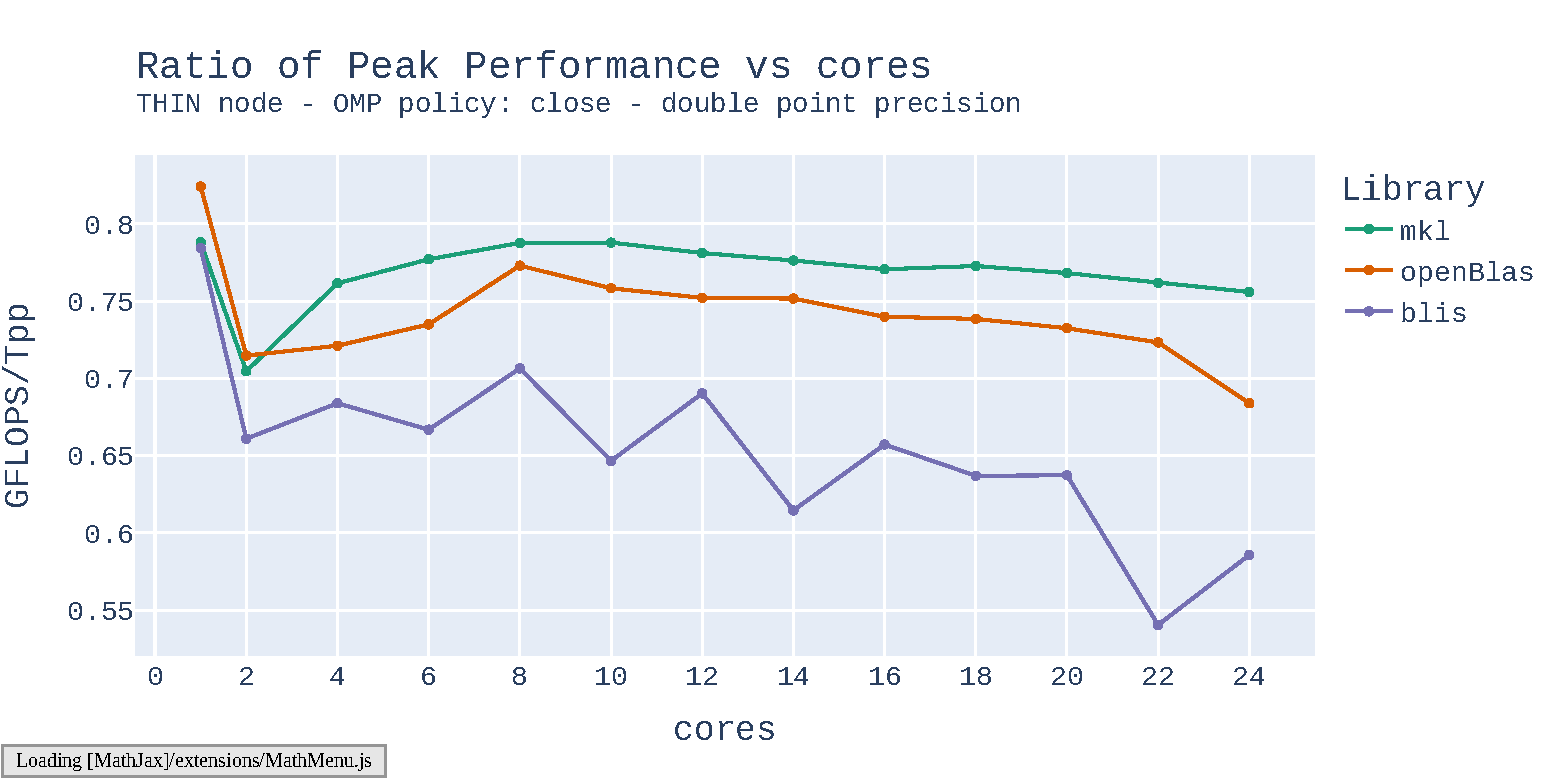
\includegraphics[width=10cm, height=6cm]{./images/fixed_size_thin_double_gflops_close_ratio.pdf}
\caption{\label{fig:fixed_size_thin_double_close} Results of DP matrix-matrix multiplication 
    as the number of cores increase, using close policy. \texttt{MKL} and \texttt{OpenBLAS}
perform the best.} 
\end{figure}

Similarly to the case of single precision, \texttt{MKL} is able to achieve around 
$\sim 75\%$ of $T_{pp}$. However, \texttt{OpenBLAS} suffers from a bit of performance 
degradation compared to the SP case. 

Once again, we notice the immediate drop in performance as soon as we use 2 cores, 
which is probably caused by the close policy. 

\begin{figure}[H]
% \centering
\hspace*{-2.5cm}
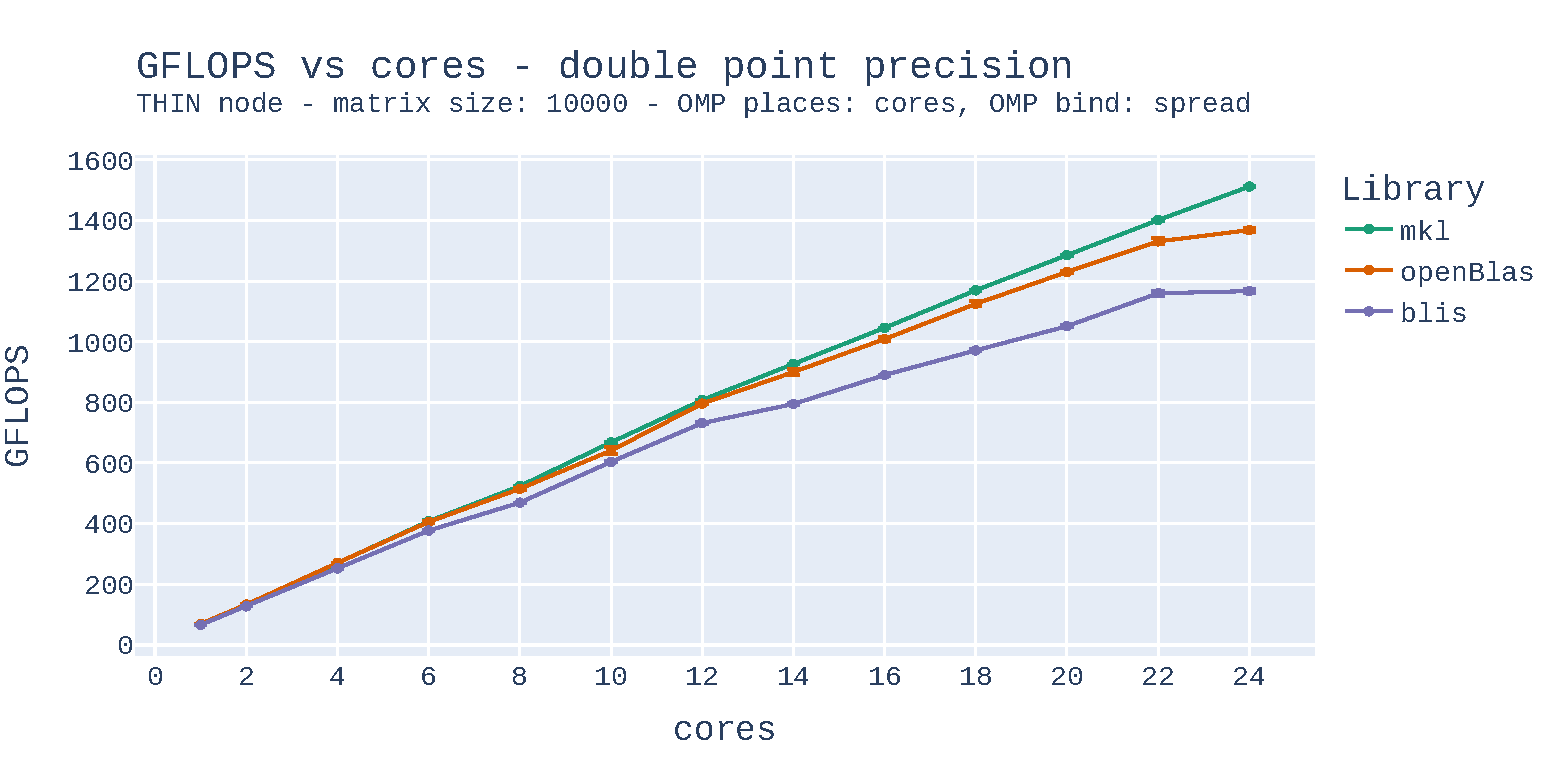
\includegraphics[width=10cm, height=6cm]{./images/fixed_size_thin_double_gflops_spread.pdf}
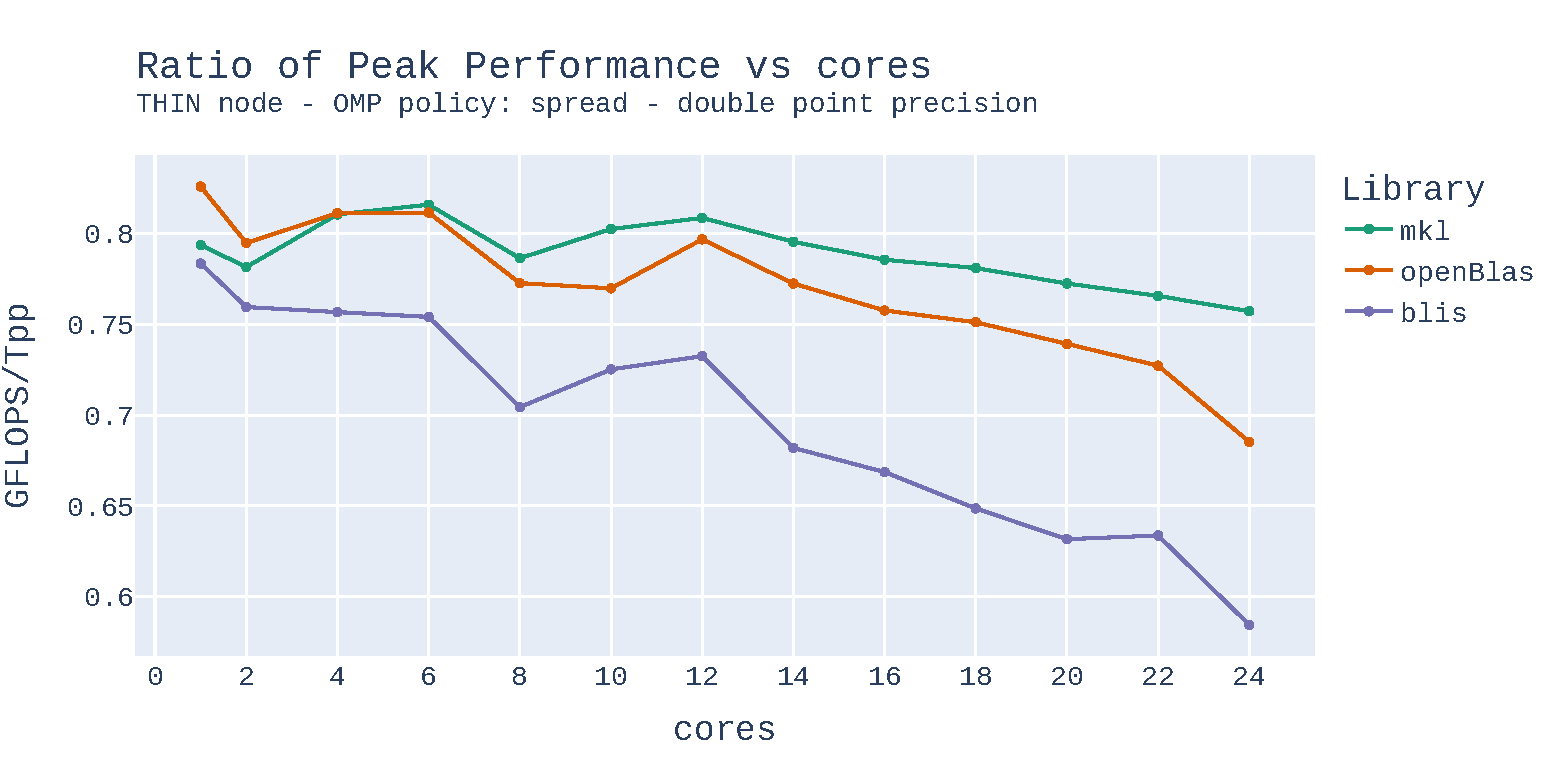
\includegraphics[width=10cm, height=6cm]{./images/fixed_size_thin_double_gflops_spread_ratio.pdf}
\caption{\label{fig:fixed_size_thin_double_spread} Results of DP matrix-matrix multiplication 
as the number of cores increase, using spread policy.}
\end{figure}

The analysis and discussion is very similar to the case of single point precision. 
We no longer see the drop at 2 cores, which is due to better resource usage from 
the beginning. Compared to the close policy, there is a slightly better performance 
for this scenario.

As usual, \texttt{MKL}, which is Intel-based, performs the best, 
closely followed by \texttt{OpenBLAS}, and finally, \texttt{BLIS}, which performs the worst. 

Finally, we analyze EPYC nodes.

\subsubsection{EPYC Nodes}

Considering the results obtained in the first part of the exercise, we expect 
that \texttt{MKL} won't be the dominating library anymore since we are using 
an AMD architecture. We also expect some more fluctuation in performance among 
the libraries, similarly to how there was a dependency on the matrix size. 

Furthermore, since we obtained low performance with matrices up to $20000$, using 
all 128 cores, we don't expect an asymptotic improvement. What may happen however,
is that when we use less cores, the performance will be much better compared 
to the theoretical peak performance (per number of cores this time).

We begin by analyzing the SP case with close policy.

\begin{figure}[H]
% \centering
\hspace*{-2.5cm}
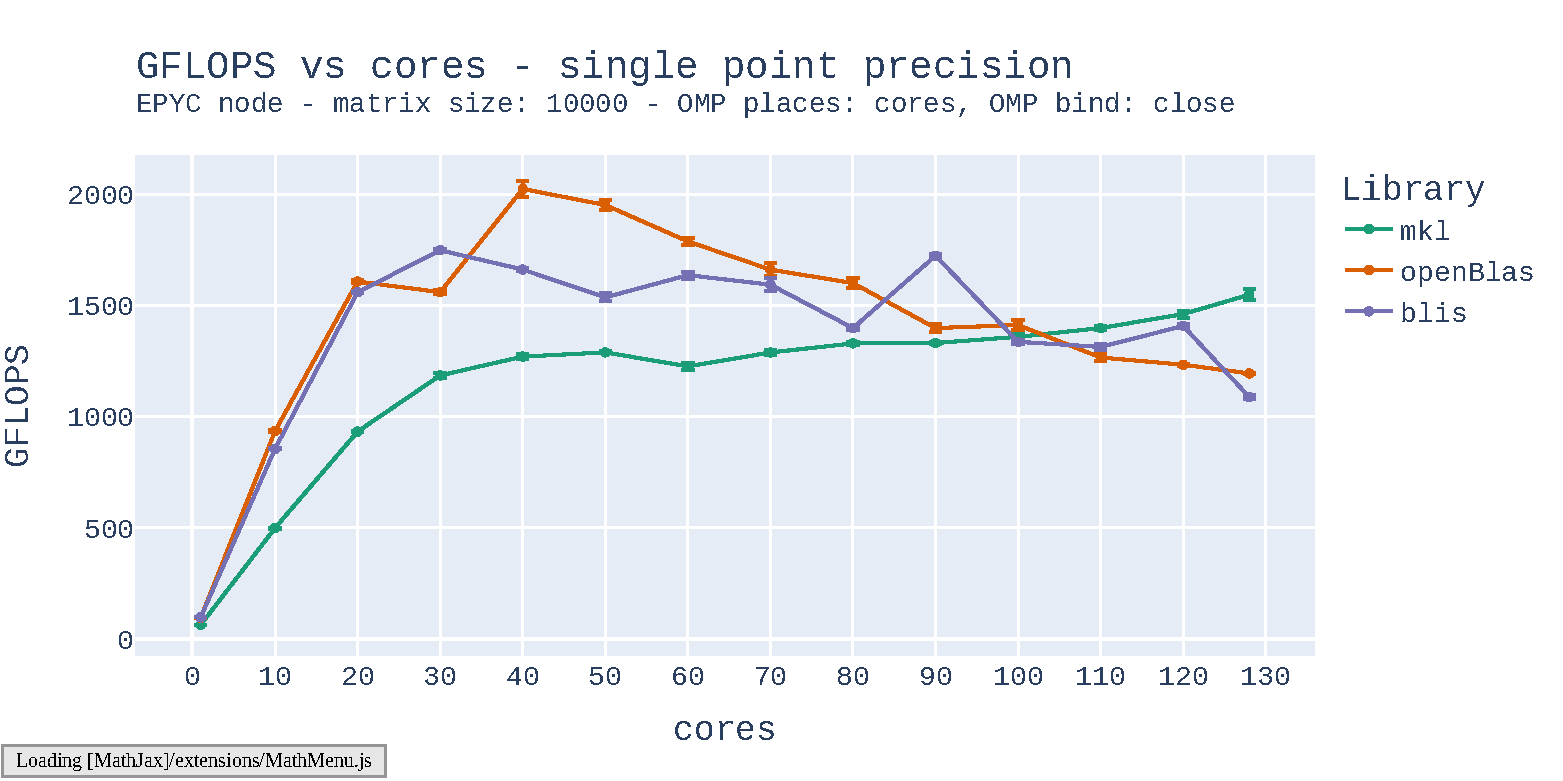
\includegraphics[width=10cm, height=6cm]{./images/fixed_size_epyc_float_gflops_close.pdf}
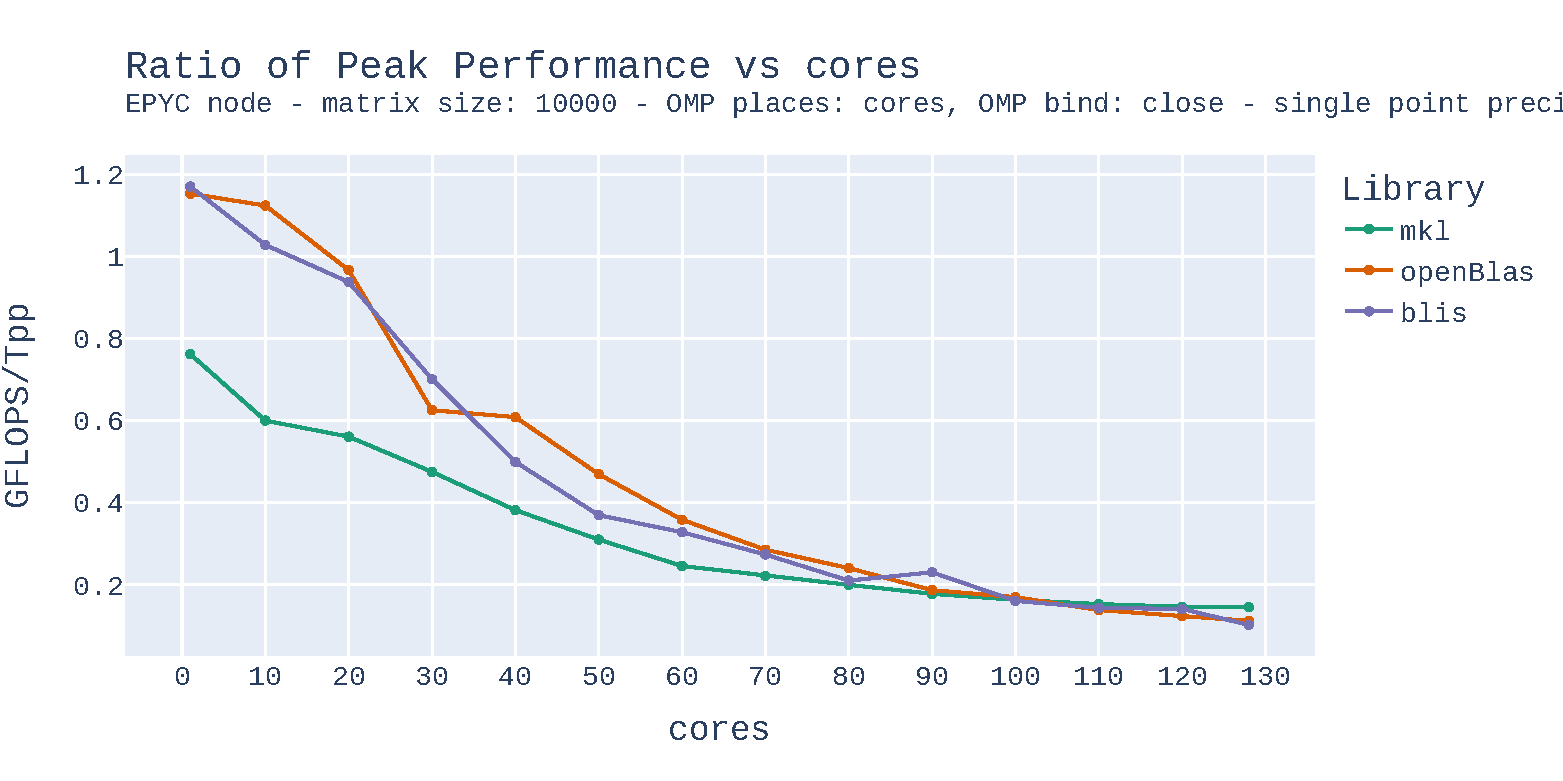
\includegraphics[width=10cm, height=6cm]{./images/fixed_size_epyc_float_gflops_close_ratio.pdf}
\caption{\label{fig:fixed_size_epyc_float_close} Results of SP matrix-matrix multiplication 
as the number of cores increase, using close policy. The best performance is obtained 
by \texttt{OpenBLAS} with 40 cores.}
\end{figure}

Looking at the graph, we see that the best absolute performance is obtained by 
\texttt{OpenBLAS} at $40$ cores, however, this is only $\sim60\%$ of $T_{pp}$. 
On the other hand, for $10-20$ cores, the performance almost on part with $T_{pp}$. 
This tells us that to fully exploit the machine as intended, with a matrices of size 
$10000$, we only need a handful of cores.

This information is consistent with our previous hypothesis that to fully exploit 
an EPYC node, we need to consider much larger matrices. 

An immediate consequence of this observation, is that as we use more and more cores, 
the performance deteriorates considerably. When we use the full node, the 
performance is $\sim20\%$ of $T_{pp}$, which is higher than what we obtained for 
the first part of the exercise.

Contrary to what happens in THIN, we do not notice any severe drops in performance 
which could be due to the close policy mapping. However, this will be more 
noticeable once we analyze what happens when we use the spread policy.

Now we analyze the SP case using spread policy.

\begin{figure}[H]
% \centering
\hspace*{-2.5cm}
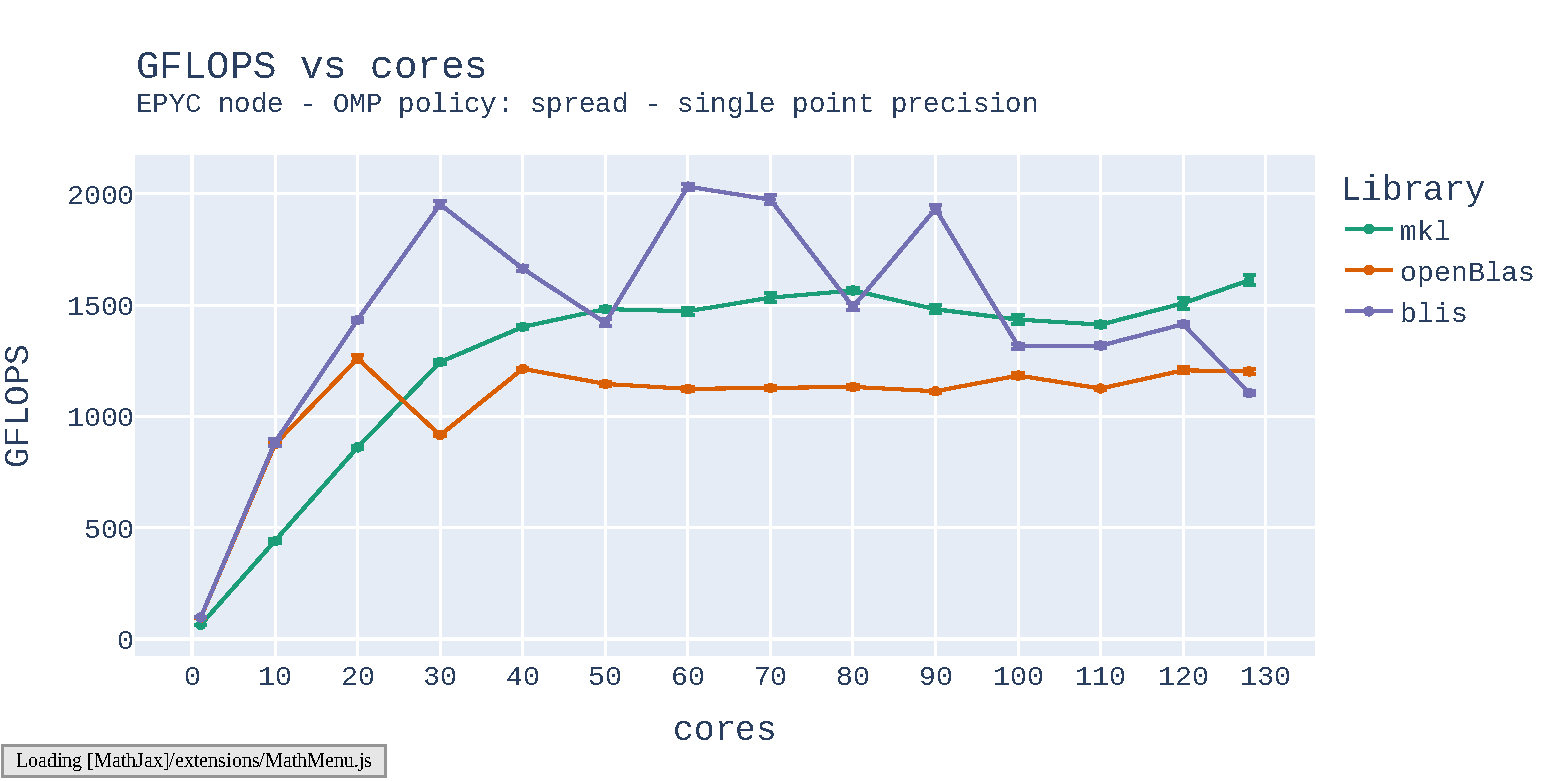
\includegraphics[width=10cm, height=6cm]{./images/fixed_size_epyc_float_gflops_spread.pdf}
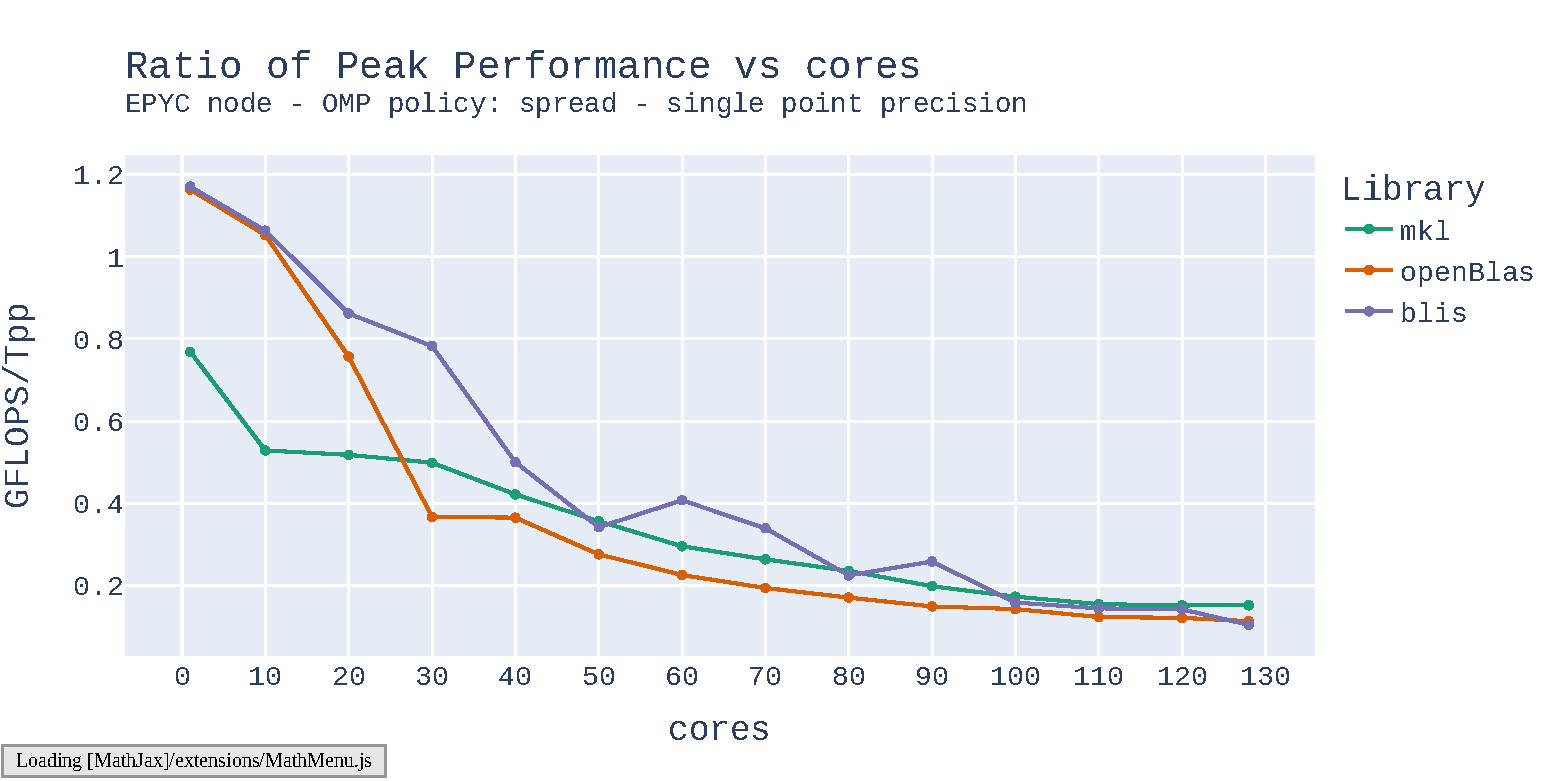
\includegraphics[width=10cm, height=6cm]{./images/fixed_size_epyc_float_gflops_spread_ratio.pdf}
\caption{\label{fig:fixed_size_epyc_float_spread} Results of SP matrix-matrix multiplication 
as the number of cores increase, using spread policy.}
\end{figure}

There is a big change. The first thing is that now \texttt{BLIS} obtains the best 
performance, although it suffers from considerable fluctuations. Furthermore, 
\texttt{OpenBLAS}, which used to perform the best, now performs the worst out of 
all three libraries.

We also notice that using the spread policy causes both \texttt{MKL} and \texttt{BLIS}
to improve and \texttt{OpenBLAS} to worsen. This is interesting because it seems 
to suggest that the latter library is better able to handle resource contention 
while the first two are better at fully exploiting resources.

Once again, we notice that as we use more cores, we get worse performance.
\\
Now we look at the DP case with close policy.

\begin{figure}[H]
% \centering
\hspace*{-2.5cm}
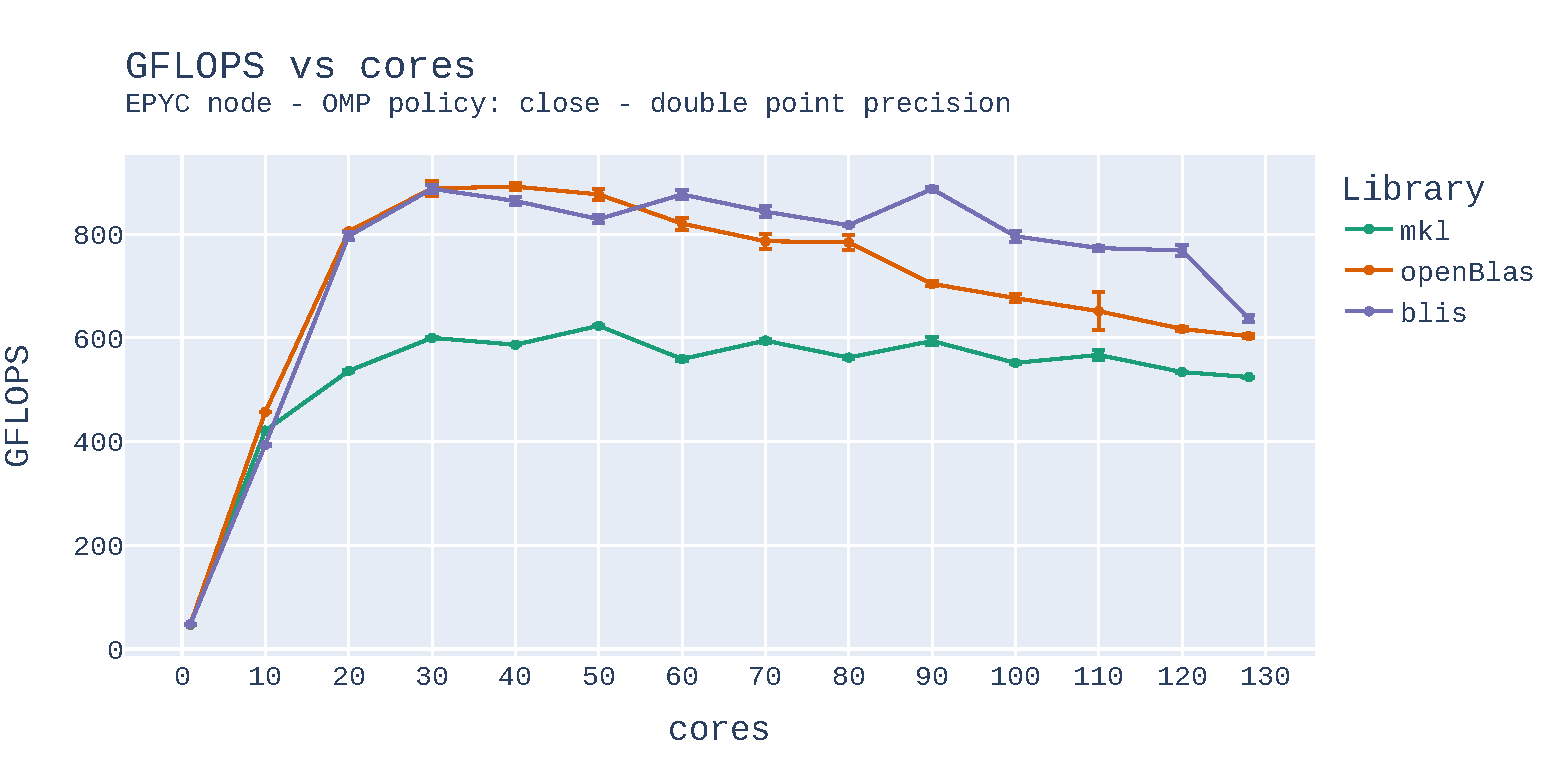
\includegraphics[width=10cm, height=6cm]{./images/fixed_size_epyc_double_gflops_close.pdf}
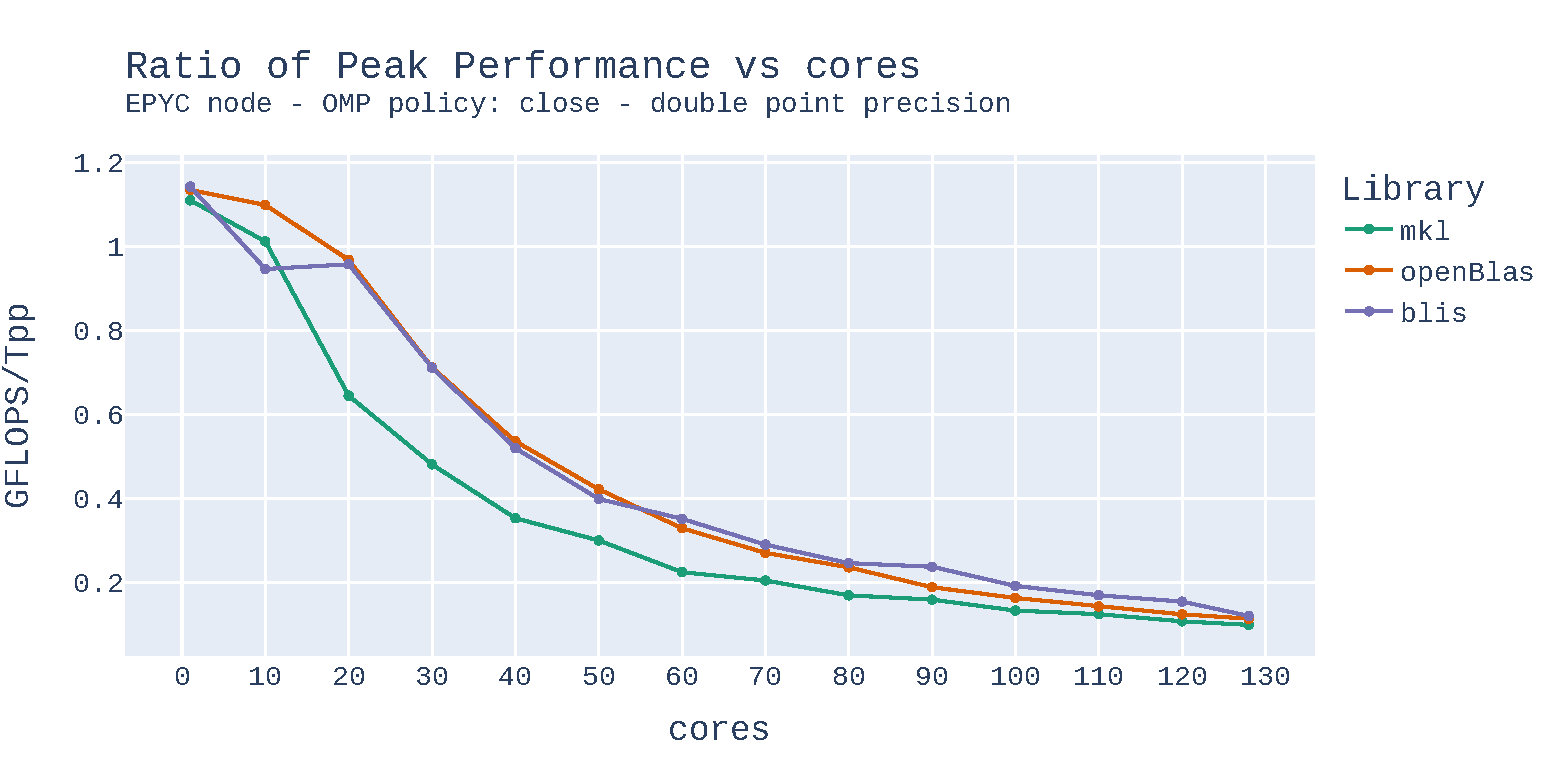
\includegraphics[width=10cm, height=6cm]{./images/fixed_size_epyc_double_gflops_close_ratio.pdf}
\caption{\label{fig:fixed_size_epyc_double_close} Results of DP matrix-matrix multiplication 
as the number of cores increase, using close policy. The best performance is 
obtained by \texttt{BLIS}, followed by \texttt{OpenBLAS}.}
\end{figure}

For double precision, using a close policy, we observe that \texttt{BLIS} 
performs the best for many cores, while for the first 64 cores, it performs close 
to \texttt{OpenBLAS}, which is the best. \texttt{MKL} peforms the worst.
\\

Finally, we analyze the DP case with spread policy.

\begin{figure}[H]
% \centering
\hspace*{-2.5cm}
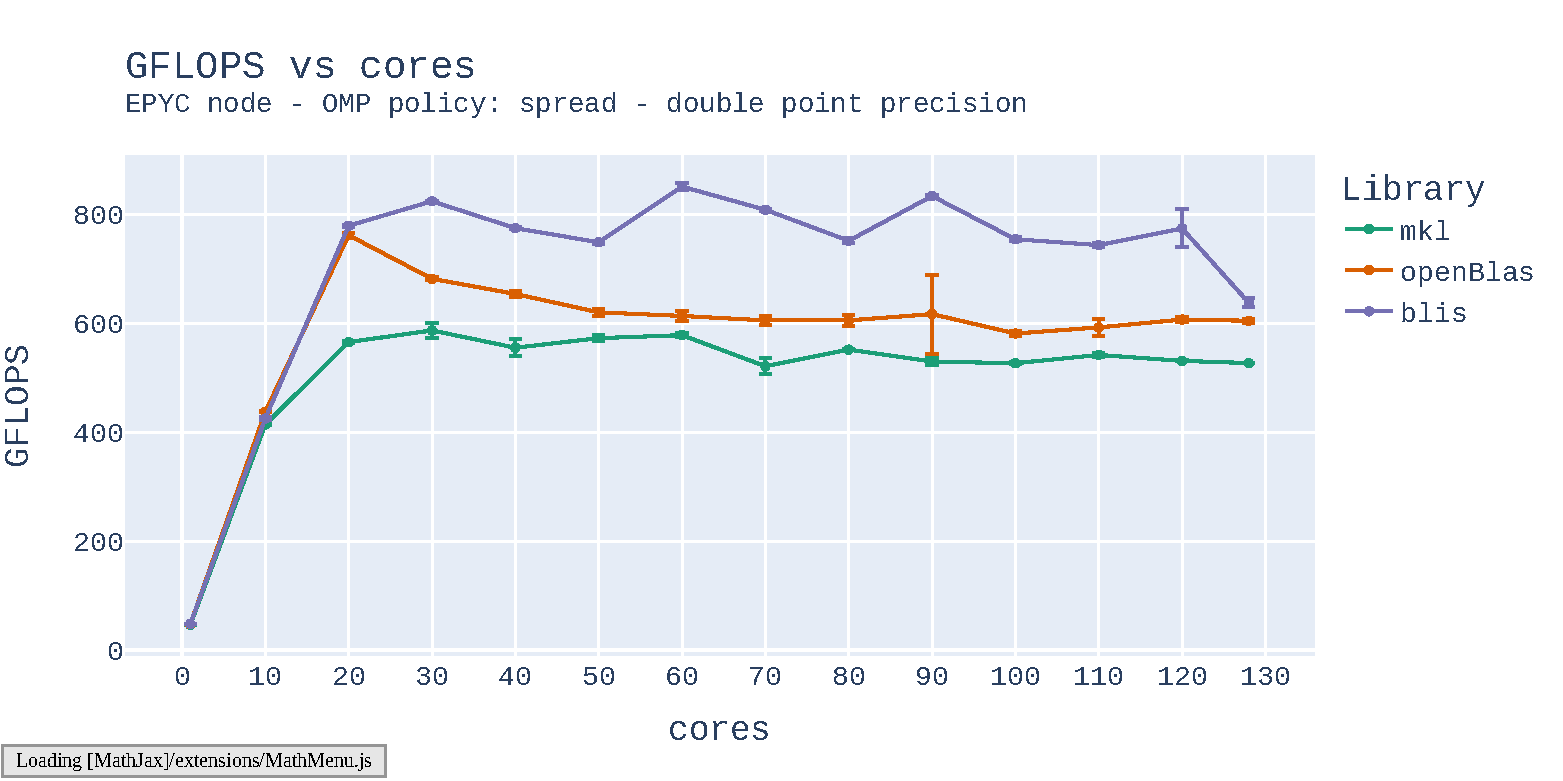
\includegraphics[width=10cm, height=6cm]{./images/fixed_size_epyc_double_gflops_spread.pdf}
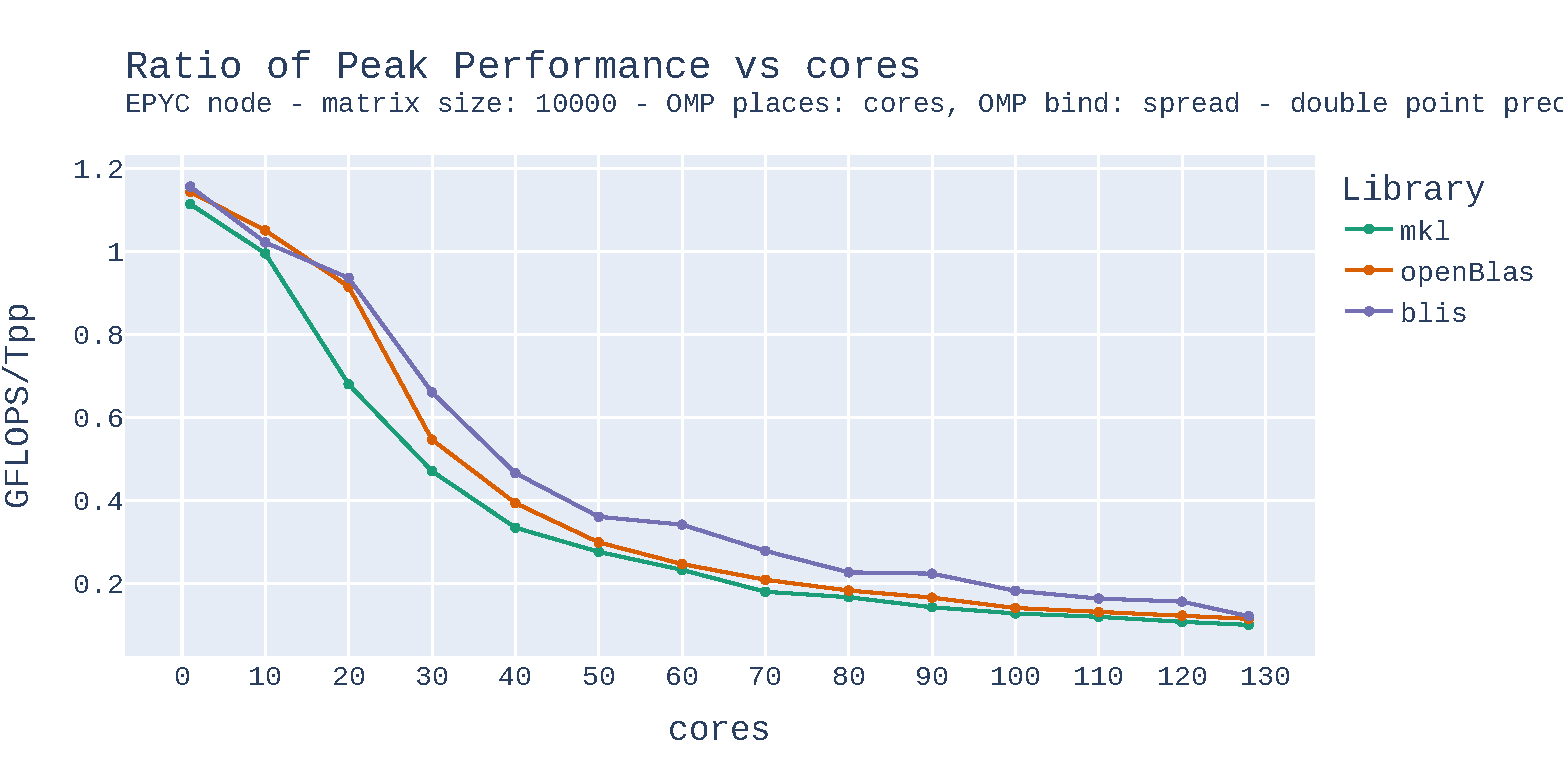
\includegraphics[width=10cm, height=6cm]{./images/fixed_size_epyc_double_gflops_spread_ratio.pdf}
\caption{\label{fig:fixed_size_epyc_double_spread} Results of DP matrix-matrix multiplication 
as the number of cores increase, using spread policy.}
\end{figure}

Using a spread policy makes the gap between \texttt{BLIS} and \texttt{OpenBLAS} much 
wider. Also, \texttt{BLIS} seems to be more capable at maintaining the throughput 
as the number of cores are increasing. Of course, this means however, that the 
peformance compared to the theoretical peak is deteriorating.

\section{Conclusion}

After analyzing the results, we can state many conclusions. The first and most 
obvious one, is that it is better to use Intel-based implementations for Intel 
machines. This is evidenced by the fact that \texttt{MKL} consistently performed
the best in all scenarios for THIN, although it was closely followed by 
\texttt{OpenBLAS}. 

Next, if we are dealing with non-Intel architecures, such as EPYC, it is not 
advisable to use \texttt{MKL}, as it consistenly underperforms compared to 
\texttt{OpenBLAS} and \texttt{BLIS}. We also notice that \texttt{OpenBLAS} and 
\texttt{BLIS} behave completely differently, depending on the mapping policy we 
use.

We find that for matrices up to $20000$, THIN nodes are able to achieve 
$\sim 75\%$ of $T_{pp}$, with \texttt{MKL} and \texttt{OpenBLAS}. However, 
such matrix dimensions are to small to be able to fully exploit an EPYC node 
which has 128 cores. In fact, in all of our experiments, we are unable to obtain 
more than $20\%$ of the $T_{pp}$ of the full node.

Finally, as an improvement to this exercise, it would be very interesting to 
analyze what happens with an EPYC node, using matrices of size $50000$ or bigger 
perhaps, to understand whether we can obtain better performance in this case.

\chapter{Conway's Game of Life}


\section{Introduction}

This exercise is devoted to implementing a scalable version of Conway's Game of 
life\cite{conway}. The game consists of a $k\times k$ grid, where each cell 
$\mathcal{C}$, at position $(i,j)$, can be "alive" or "dead".

The grid evolves over time by looking at each cell's  eight nearest 
neighbors and observing the following rules: 

\begin{itemize}
    \item A dead cell with exactly three live neighbors comes to live (\textit{birth}).
    \item A live cell with two or three neighbors stays alive (\textit{survival}).
    \item A dead or live cell with less than two or more than three neighbors dies 
        or stays dead (\textit{death}).
\end{itemize}

These seemingly simple rules give rise to many interesting behaviors and 
patterns\cite{conway_patterns}. 

There exist two methods to evolve the grid: \texttt{static} and \texttt{ordered}
evolution. In \texttt{static} evolution, we freeze the state of the entire grid 
$\mathcal{G}_t$ at time step $t$, and compute $\mathcal{G}_{t+1}$, separately, 
while looking at $\mathcal{G}_t$. This corresponds to maintaining two buffers, 
one for the current generation and the other for the new generation.

On the other hand, in \texttt{ordered} evolution, we start from a specific cell, 
usually in position $(0,0)$ (top left), and update the elements inplace. This 
means that the state of each cell depends on the evolved state of some of its 
neighbors. We call this "ordered" evolution, because the choice of starting 
point, and the order in which we evolve the grid, lead to different results.
In this scenario, the state of each cell instrinsically depends on the history of 
evolution of \textit{all} the cells before it. 

Our implementation must satisfy the following requirements: 

\begin{enumerate}
    \item Randomly initialize a square grid ("playground") of size $k \times k$ 
        with $k \geq 100$ and save it as a binary PGM\cite{pgm} file.
    \item Load any binary PGM file and evolve for $n$ steps.
    \item Save a snapshot during the course of evolution with a frequency $s$, 
        where $s=0$ means saving only at the end. 
    \item Support both \texttt{static} and \texttt{ordered} evolution.
\end{enumerate}

Lastly, it must use both MPI\cite{mpi} and OpenMP\cite{omp} (OMP) to paralellize 
the computations and be able to process grids of considerably high dimensions. 

Using our implementation, we will perform a study of the scalability of our code 
in three cases: 
\begin{enumerate}
    \item Strong OMP scalability: Using a grid of fixed dimensions, we fix the 
        number of MPI processes to one per socket and progressively increase 
        the number of OMP threads.
    \item Strong MPI scalability: Using a grid of fixed dimensions, we increase 
        the number of MPI processes, using only 1 OMP thread per process. We use 
        the largest amount of nodes possible.
    \item Weak MPI scalability: Changing the grid dimensions to keep the work per 
        process constant, we use one MPI process per socket, with enough OMP 
        threads to saturate the cores in the socket, and slowly increase the 
        number of MPI processes among multiple nodes.
\end{enumerate}

\section{Methodology}

In this section, we briefly describe some of the important choices for the 
implementation, as well as their implications. We will proceed by layers, 
tackling the more abstract and higher level problems first and then slowly 
going into detail about more technical choices. 

The first most important step is to think about how to paralellize the problem 
in order to use MPI and OMP properly.

Since programs in MPI need to be written completely with paralellization in mind 
from the start, we must begin to conceptualize the problem in an encapsulated 
manner from the beginning.

At a high abstract level, we must make two important choices: 

\begin{enumerate}
    \item How we will decompose the problem. 
    \item How we will perform the IO. 
    \item How to mix MPI and OMP.
\end{enumerate}

How we solve the first problem is of fundamental importance to ensure that our 
program is scalable and efficient. Also, it has important consequences on the 
type of paralellism we will need to use. 
On the other hand, the second problem will determine the organizational paradigm 
that we will use in our code, as we will see later.
Finally, the third solution will determine the effectiveness of our hybrid code.

We briefly discuss both of these topics more in depth in the following 
subsections.

\subsection{Decomposition}

To exploit paralellism, we must first identify the concurrency in our 
application and then apply some form of decomposition. The two most important 
types of decomposition are \texttt{domain} and \texttt{functional} decomposition. 

In \texttt{domain} decomposition, multiple workers are performing the same set of 
instructions on different portions of data (SIMD). In \texttt{functional} 
decomposition, workers are performing different instructions on possibly 
different data (MIMD). 
 
In the case of \texttt{static} evolution, each cell can be updated 
independently from each other, as long as we have acccess to its neighbors. 
Therefore, one immediately obviously form of paralellism is for each MPI 
process to process a "part" of the whole grid. This is an example of \texttt{domain}
decomposition, and it is shown below:

\begin{figure}[H]
\centering
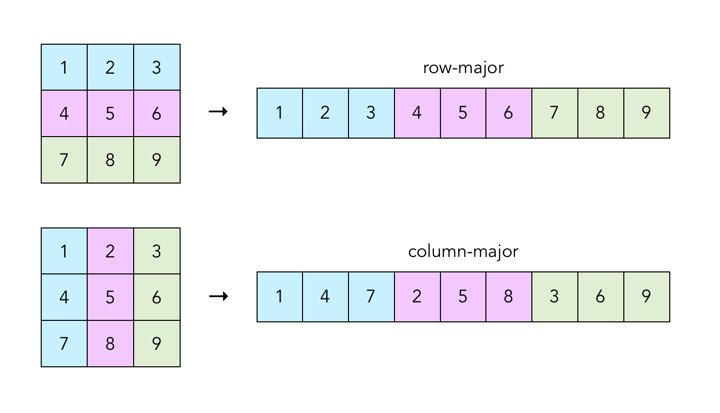
\includegraphics[width=10cm, height=5cm]{./other_images/arraydecomposition.jpg}
\caption{\label{fig:decomposition} Decomposition of an array among three processes. 
Although the array is conceptualized as a 2D structure, internally, for efficiency, 
it is represented as a 1D contigous block of memory.}
\end{figure}

However, we need to decide how to split the grid. We can do a 1D decomposition by 
"stripes", as shown in image \ref{fig:decomposition} or a 2D decomposition by 
"blocks". It is known that a 2D decomposition is more efficient as it 
can exploit more bandwidth as more workers will send shorter messages 
contemporarily. However, it is more complicated both from an implementation 
point of view and worse for memory access.

Let's talk briefly about this second aspect. Although we talk about the 
grid as a 2D array, internally, for efficiency, it will be represented as a 1D 
array. 

If we do a 1D split, each process will work on a thick strip of data which 
continuous in memory. On the other hand, if we do a 2D split, each process will 
work on a block of memory which is not contiguous and located every certain 
"jumps" in the 1D array. As a consequence, as each process traverses its block 
of the grid, it will have more cache misses compared to the 1D case where 
we perform a simple a linear access. This is more easily visualized in 
the following image:

\begin{figure}[H]
\centering
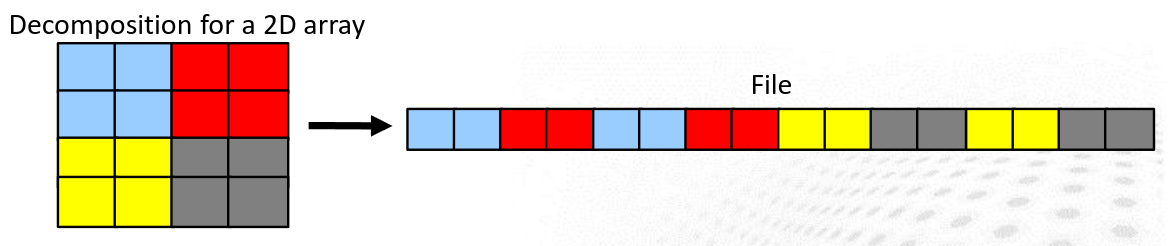
\includegraphics[width=12cm, height=4cm]{./other_images/2d_decomposition.png}
\caption{\label{fig:2ddecomposition} 2D decomposition of a grid. As we can see, 
each process needs to deal with non-contiguous memory.}
\end{figure}


Therefore, for reasons stated above, and for simplicity and readability, we 
decided to use the 1D splitting.

Lastly, we must consider how to handle halo regions. Since each process will 
process a strip - composed of 1 or more rows - of the grid, the rows at the 
boundary of the strip must be handled with special attention. These rows - 2 per 
process - need information that is contained in the grid of other processes.
Therefore, we need to allocate some extra space for these additional rows, and 
set up message passing between processes to handle the exchange of these 
boundary rows, also known as \texttt{halo} regions.

Below we show the idea:

\begin{figure}[H]
\centering
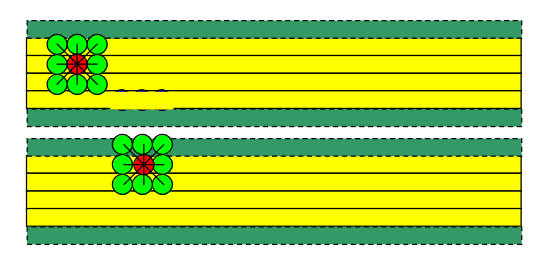
\includegraphics[width=4cm, height=3cm]{./other_images/stencil.png}
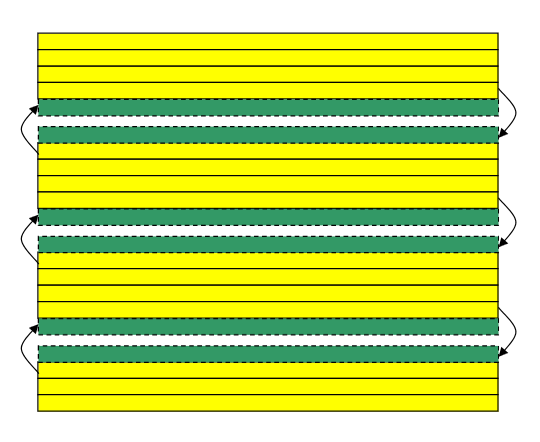
\includegraphics[width=8cm, height=5cm]{./other_images/halo_exchange.png}
\caption{\label{fig:haloexchange} On the figure in the left, we can see that 
we can process cells that are internal with no problem. However, at the boundary 
we need information that belongs to another process. Therefore, we allocate 
some extra space and do a halo exchange as shown in the figure on the right.}
\end{figure}

Finally, in the case of \texttt{ordered} evolution, we cannot update each cell 
independently, since we modify the elements inplace in an ordered fashion. 
Therefore, we cannot parallelize this process. The only thing that we can do, is 
use MPI to be able to process much bigger grids than we could in a conventional 
computer. In this case, each process will compute its part of the grid 
\textit{in order}, rather than in parallel. So process 0 will update its portion, 
and send the updated row to process 1, and so on. Of course, each process needs 
the appropriate halo regions. 

\subsection{MPI IO}

The problem specifications require that we must save the grid with a certain 
frequency $s$. There are multiple ways to achieve this, and they all have 
important implications on the scalability of the code. 

The simplest way is for each process to write its part of the grid to a 
separate file. This however, is extremely messy as we loose the flexibility 
of using a different number of processes between separate runs. More importantly, 
for a large number of processes, the filesystem will not be able to handle all 
these requests and will be completely overloaded and possibly crash. This means 
that for $P>>1$ we would have very serious problems, which is undesirable, since 
we wish to use as many processes as we want/have.

The second solution, is to use a master-slave approach. In this paradigm, one 
process is designated as the master process, while all the other are its slaves. 
The master will coordinate the IO, and with a frequency $s$, it will collect 
information from all the slaves, and take care of writing everything to a file. 
This approach, although very common, is not scalable, as each process needs to 
send its part of the grid to the master process. So for $P>>1$, the bottleneck 
will be in the communication. 

Lastly, the third, and best solution, is to use \texttt{MPI IO}, which was meant to handle 
exactly this problem. The idea behind \texttt{MPI IO} is very similar to message passing. 
Each process will call a collective function to read/write its part of the grid
and the MPI implementation will take care of exploiting the parallel filesystem
and reducing the amount of read and write operations. Furthermore, this is 
the only solution that takes advantage of the parallel filesystem which allows 
for a unified logical view of the file, while allowing the file to be stored 
in physically different locations. This is very advantageous for scalability 
since many processes can contemporarily write in different physical locations, 
which increases the throughput of the program. We note that this is a form 
of \texttt{functional} decomposition.

Notice that this aspect is independent of the type of evolution.

\subsection{Mixing MPI and OMP}

Now that we have discussed at an abstract level how to distribute the workload 
among the MPI processes, we need to think about how to integrate OMP to obtain 
a hybrid implementation. 

In \texttt{static} evolution, since each process can update its part of the grid 
independently, the most natural approach is to use OMP to parallelize this 
computation. For this, there are a few options. 

The simplest option, is that each MPI process will spawn a parallel region at 
\textit{each} iteration $t$ to accelerate its computations.

Another, more advanced approach, is to use \texttt{MPI\_THREAD\_MULTIPLE}. In 
this mode, each OMP thread can make an MPI call contemporarily. This mode must 
be handled with care but it will enable us to create a \texttt{single} parallel
region, as we will see later. 

We implemented both cases to do some comparisons. 

Finally, for \texttt{ordered} evolution, we cannot use OMP, because the update 
depends on the order, and it is intrinsically serial.

\section{Implementation}

In this section, we discuss the most technical details of our implementation, 
from the datatypes used, to compiler keywords, to optimization of branches, to 
memory allocation, and optimization of for loops. We will also describe how to 
use the code, what software stack is needed, and what tools were used.

Our implementation was done in C, so we will have to manually handle all 
memory aspects. This gives us great control in to what we are doing. 

\subsection{State representation}

We begin by discussing how to represent data. Since each cell can be alive (1) 
or dead (0), theoretically, we need a single bit to represent the state. This 
means that every byte of data can represent the state of 8 cells. However, 
this approach is complex since we need to do a lot of bit manipulation to 
access the information of each cell. This will also make the code less 
readable and longer. 

The next best idea, which we used, is to use the smallest datatype possible, 
i.e a \texttt{char}, which is 1 byte, to represent the state of a single cell.
In this way, we are less memory efficient, but we gain in readability and ease 
of implementation. In particular, we use an \texttt{unsigned char} which 
is of the same size, however, in this way, the compiler can possibly optimize 
the operations since it doesn't need to keep track of the sign.

All of our implementations contain the following macros:
\begin{lstlisting}[language=C++]
#define DEAD 0 
#define ALIVE 1
\end{lstlisting}

\subsection{Distributing the grid among MPI processes}

Given a $k \times k$ grid, we need to tell each MPI process how many rows it must 
deal with.
To do this we can divide the total number of rows by the number of processes, i.e 
the size of the MPI Communicator, and distribute the remainder among a subset 
of them.

This is done through a common trick:
\begin{lstlisting}[language=C++]
    my_rows = total_rows/size + 1*(rank<(total_rows%size));
\end{lstlisting}

In this way, all processes will have an equal workload, except for some ranks 
which will have to process one more row.

\subsection{Allocating data}

Now that we have determined how many rows each process has to deal with, each 
rank must allocate the appropriate memory in heap to store its portion of the 
grid.

In \texttt{static} evolution, we need to keep two buffers, one for the current 
generation, and one for the next one. We look at the previous generation as we 
update the new generation. In \texttt{ordered} evolution, we only have one buffer, 
and we update each cell inplace as we traverse the array.

As mentioned previously, it is not efficient to allocate a 2D array, although it 
is more naturally aligned with the problem statement. This is because 2D arrays 
are not necessarily contiguous in memory and we also have an overhead of 
following pointers.

Therefore, we allocate 1D arrays which are contiguous in memory and we use 
a macro to be able to access the array as if it were a 2D structure. 

Lastly, for each process, we need to allocate two additional rows to accomodate 
the halo rows. Also, to optimize for cache access, we explicitly align the data 
to the cache line size of THIN and EPYC nodes, which are 64 Bytes.

This can be seen in the following snippet:

\begin{lstlisting}[language=C++]
// defining cache line size
#define CACHE_LINE_SIZE 64
// macro to access data in 2D fashion
#define DATA(i,j) (data[(i)*cols + (j)])

... 

// aligned allocation
data = (unsigned char *) aligned_alloc(CACHE_LINE_SIZE, (my_rows + 2) * cols);
\end{lstlisting}

Of course, for \texttt{static} evolution, we perform two such allocations.

\subsection{PGM Files - Header}

Now that we have discusses how we perform the allocation, we briefly discuss 
PGM binary files. 

PGM, or Portable Grey Map, are portable binary files composed of a header and 
of binary data. In our case, the header is the following line: 

\begin{verbatim}
P5 {rows} {cols} {maxval}\n
\end{verbatim}

The \texttt{P5} is a magic number that states we are using a PGM file of binary 
data where each byte corresponds to a pixel in the image. The color 
is interpreted according to the \texttt{maxval} value. Without going 
into too much detail, by setting \texttt{maxval} to one, we are establishing that 
1's will represent be drawn as white (alive) and 0's will be drawn as black 
(dead).

Whenever we save a snapshot of the evolution, we need to write this header. 
This will be done by one single process - rank 0. 

Also, as we will see later, to use MPI IO, we need to find out the length of 
this header in bytes. All these operations are performed in the following snippet:

\begin{lstlisting}[language=C++]
#define HEADER_FORMAT_STRING "P5 %lf %lf %d\n"
#define MAX_VAL 1

... 

// We get the header size 
header_size = snprintf(NULL, 0, HEADER_FORMAT_STRING, rows, cols, MAX_VAL);

// allocate the string
header = malloc(header_size + 1)

// write the header into the string
sprintf(header, HEADER_FORMAT_STRING, rows, cols, MAX_VAL);
\end{lstlisting}

We will use the header size in MPI IO, in the next section.

\subsection{MPI IO}

As discussed above, MPI IO is the best choice to handle the IO when we are 
dealing with many processes. It takes advantage of the parallel file system 
to write in multiple locations at once, while keeping a logically unified 
view of the file. In this way, we avoid the bottleneck of having to send the grid 
back to the master or overloading the filesystem with too many posix calls.

Below we list the code snippet that we used and then discuss the relevant details. 
\begin{lstlisting}[language=C++]

void save_grid(char * restrict fname, MPI_Comm comm, int rank, char * restrict header, unsigned long int header_size, MPI_Offset offset, unsigned char * restrict data, unsigned long int my_rows, unsigned long int cols)
{

    MPI_File fh;

    // Opening the file in MPI_MODE_WRITEONLY or MPI_MODE_CREATE_ONLY
    const int err = MPI_File_open(comm, fname, MPI_MODE_WRONLY | MPI_MODE_CREATE, MPI_INFO_NULL, &fh);

    // Check that the file was opened correctly
    if(err != MPI_SUCCESS)
    {
        fprintf(stderr, "Error opening %s\n", fname);
        MPI_Abort(MPI_COMM_WORLD, err);
    }
    
    if(rank == 0)
    {
        // we specify the file handle, the byte where we write, what we write, 
        // the length of what we write, the data type of what we write, and the 
        // status of the writing.
        MPI_File_write_at(fh, 0, header, header_size, MPI_CHAR, MPI_STATUS_IGNORE);
    }

    MPI_File_write_at_all(fh, offset, data + cols, my_rows*cols, MPI_CHAR, MPI_STATUS_IGNORE);

    MPI_File_close(&fh);
}

\end{lstlisting}

First, all processes call the \texttt{MPI\_File\_open()} routine to open the file. 
The file is opened in \texttt{MPI\_MODE\_WRONLY} for write only and 
\texttt{MPI\_MODE\_CREATE} to create the file if it does not exist already.

Then, we choose rank 0 to write the header of the PGM file. We use the MPI function
\texttt{MPI\_File\_write\_at()} which allows us to specify at what position in the 
file, in bytes, the data must be written. 

For the header, we will write at the beginning of the file, so at byte 0. The 
rest of the arguments are explained in the snippet.

Finally, for writing the grid, we will use the collective version of 
\texttt{MPI\_File\_write\_at()}, namely \texttt{MPI\_File\_write\_at\_all()}. 
This function is called by all the processes. Internally, the MPI 
implementation will perform this operation in the most efficient way possible.

The arguments are the same as the non-collective version. 

The only thing we need to explain, is how we find the byte offset for each 
process. 

We first find the \texttt{row} offset, i.e. which row to start writing from, 
through the following function:

\begin{lstlisting}[language=C++]
unsigned long int get_my_row_offset(unsigned long int total_rows, int rank, int size)
{
    // returns the offset from which the rank must get its rows 

    // for example: for rank 0, the offset will be zero as it will read 
    // my_rows(of rank 0) from the start. However, rank 1 will have to read 
    // after the rows that rank 0 handles (accounting for the remaineder), 
    // and so on.

    // nrows is the interger division between total_rows and size
    unsigned long int nrows = total_rows/size;
    unsigned long int remainder = total_rows%size;

    // The idea is the following, if the division was pefect, we would do 
    // nrows * rank. However, we still need to account for the remainder.
    // For remainder processors (starting to count from rank 1 because rank 0 
    // just gets 0 as offset), we simply need to add rank to the offset. 
    // If we are dealing with a process id which is greater than the remainder, 
    // then we simply need to add the whole remainder.
    
    unsigned long int my_offset = nrows*rank
        + rank*(((unsigned long int) rank) <= remainder) 
        + remainder*(((unsigned long int) rank) > remainder);

    return my_offset;
}
\end{lstlisting}

We illustrate with a brief example. Suppose we have a $14\times 14$ grid and four 
ranks. The interger division is $3$ and the remainder is $2$. Since the 
remainder of the division is $2$, two ranks, 0 and 1, will need to handle an 
extra row. 

So rank 0 will deal with $3+1=4$ rows, rank 1 will also deal with $3+1=4$ rows, 
and ranks 2 and 3 will deal with $3$ rows each.

Now, for the offset, rank 0 will just have offset 0. Rank 1 will need to shift 
by the interger division plus 1 to account for the extra row that rank 0 has. 
Similarly, rank 2 has to shift by twice the interger division, plus the extra 
row that rank 0 has and the extra row of rank 1. 

Rank 3 will have to shift by three times the interget division, plus the extra 
rows of the previous ranks. However, this time, rank 2 did not have an extra 
row. So rank 3 just needs to account for \textit{total} extra rows, which is 
equal to the remainder. 

This sounds complicated, but it is simple once one works through a few examples.

Since the offset for the MPI functions is in bytes, to get the final 
offset, we first multiply the row offset by the number of columns, and by the 
size of the datatype we use in bytes - for a char this is 1.

Then we need to add the size in bytes of the header.

\begin{lstlisting}[language=C++]
        ...

        const MPI_Offset header_offset = header_size * sizeof(char);

        const MPI_Offset my_file_offset = my_row_offset * cols * sizeof(char);

        const MPI_Offset my_total_file_offset = my_file_offset + header_offset;

        ...
\end{lstlisting}

Finally, reading of the file is done in the same exact way, replacing 
\texttt{MPI\_File\_write\_at\_all} with \texttt{MPI\_File\_read\_at\_all}. 

However, we need to have an additional step to read the header, and this is done 
through a normal \texttt{fscanf()} call.

\subsection{Updating Cells - Static Evolution}

Now we discuss how we perform the cell update for \texttt{static} evolution. 

The entire evolution process is contained inside a for loop over time steps. 
At each iteration, we had to use message passing to exchange the halo rows. This 
is done using non blocking operations to hide the latency of the communication.

\begin{lstlisting}[language=C++]
// we post send and recv requests for two halo regions.
// matrix: 
// ---------------------  row 0 (HALO)
// 010100011001100100100  row 1
// 010010000100101001111  row 2             --
// ...                                        | these rows dont need 
// 001010111110011000001  row my_rows - 1   __| halo regions
// 010010010000100101000  row my_rows
// ---------------------  row my_rows + 1 (HALO)

// send row: 1 to the previous rank
MPI_Isend(data_prev + cols, cols, MPI_CHAR, prev, prev_tag, MPI_COMM_WORLD, &prev_send_request);
// send row: my_rows to next rank
MPI_Isend(data_prev + my_rows_x_cols, cols, MPI_CHAR, next, next_tag, MPI_COMM_WORLD, &next_send_request);

// receive from prev and put in row 0 (halo region)
MPI_Irecv(data_prev, cols, MPI_CHAR, prev, next_tag, MPI_COMM_WORLD, &prev_recv_request);
// receive from next and put in row my_rows + 1 (halo region)
MPI_Irecv(data_prev + my_rows_x_cols_p_cols, cols, MPI_CHAR, next, prev_tag, MPI_COMM_WORLD, &next_recv_request);
\end{lstlisting}

Where \texttt{data\_prev} and \texttt{data} are the buffers for the previous 
and next generation, respectively. 

Next, while messages are exchanged, each process can process the internal portion of 
its grid.

Two versions were used to do this: one using a double for loop over rows and columns, 
and the other using a single for loop over cells. Later, when we tie everything 
together, we will explain the reason for these two versions.

\begin{lstlisting}[language=C++]
... 

// note we start from row 2 and finish at row my_rows - 1
for(unsigned long int row = 2; row < my_rows; ++row)
{
    for(unsigned long int col = 0; col < cols; ++col)
    {
        upgrade_cell_static(data_prev, data, row, col);
    }
}

...
\end{lstlisting}

\begin{lstlisting}[language=C++]
for(unsigned long int cell = 2*cols; cell< my_rows*cols; ++cell)
{
        unsigned long int i = cell/cols;
        unsigned long int j = cell - i*cols;
        upgrade_cell_static(data_prev, data, i, j);
}
\end{lstlisting}

Finally, at this point, there is nothing left to do, but wait until we receive 
the halo cells.

\begin{lstlisting}[language=C++]
MPI_Wait(&prev_recv_request, MPI_STATUS_IGNORE);
MPI_Wait(&next_recv_request, MPI_STATUS_IGNORE);
MPI_Request_free(&prev_send_request);
MPI_Request_free(&next_send_request);
\end{lstlisting}

We then process the first and last row of the grid (internal ones).

\begin{lstlisting}[language=C++]
for(unsigned long int col=0; col<cols; ++col)
{
    upgrade_cell_static(data_prev, data, 1, col);
}
// we only do this if we have more than one row 
for(unsigned long int col=0; col<cols*(my_rows>1); ++col)
{
    upgrade_cell_static(data_prev, data, my_rows, col);
}
\end{lstlisting}

Then, if we need to save the grid we save using MPI IO, and then we swap the 
pointers and repeat.

Apart from a few differences that we introduce with OMP later, these are the 
fundamental steps of our evolution.

The last thing is to discuss the update function itself:

\begin{lstlisting}[language=C++]
void upgrade_cell_static(unsigned char * restrict data_prev, unsigned char * restrict data, unsigned long int i, unsigned long int j)
{
    DATA(i,j) = DEAD;

    // we use ternary operators to avoid branches
    // as well as the register keyword to signal to the compiler to 
    // keep this data close

    // compute coordinates of neighbors with wrap around of dimensions
    register unsigned long int jm1 = j==0 ? cols-1 : j-1;
    register unsigned long int jp1 = j==(cols-1) ? 0 : j+1;
    // for rows, wrapping is ensured by the presence of halos
    register unsigned long int im1 = i-1;
    register unsigned long int ip1 = i+1;
    
    // we fetch the neighbors with 8 different instructions to saturate pipelines.
    // We access first the neighbors that are already most likely already 
    // in cache due to previous updates.
    unsigned char tmp0=DATA_PREV(im1, jm1);
    unsigned char tmp3=DATA_PREV(i,jm1);
    unsigned char tmp5=DATA_PREV(ip1,jm1);

    unsigned char tmp1=DATA_PREV(im1,j);
    unsigned char tmp2=DATA_PREV(im1,jp1);

    unsigned char tmp4=DATA_PREV(i,jp1);

    unsigned char tmp6=DATA_PREV(ip1,j);
    unsigned char tmp7=DATA_PREV(ip1,jp1);

    unsigned char n_alive_cells = tmp0+tmp1+tmp2+tmp3+tmp4+tmp5+tmp6+tmp7;

    DATA(i,j) = ALIVE*(n_alive_cells==3) + DATA_PREV(i,j)*(n_alive_cells==2);
}
\end{lstlisting}

The function is very simple. First, we set the cell to be dead regardless, since 
if there are less than two and more than 3 live neighbors, it dies.

Then, we calculate the coordinates of the neighbors using ternary operators to 
ensure that we wrap around the dimensions. 

Then, we use separate instructions for each neighbor to encourage pipeline 
saturation.

We aggregate the state of all the neighbors, and apply the rules. 
This version of the rules may seem off at first, but it is completely 
equivalent to the one we described, although in this way, it's a bit more efficient.

Finally, notice the \texttt{restrict} keyword for the two pointers so that the 
compiler can optimize better since it knows it will never encounter memory 
aliasing.

\subsection{Updating Cells - Ordered Evolution}

For \texttt{ordered} evolution, the idea is more complex.   

We need to make sure that ranks process their parts of the grid in an ordered 
fashion. We first show the commented snippet and then comment:

\begin{lstlisting}[language=C++]
// for ordered evolution, we cannot parallelize, and each process 
// must work on their part of the grid in serial order. 

// first, each process posts a non blocking receive operation for 
// the top halo row and the bottom halo row. 
// Since we have ordered evolution each process will then wait 
// until the top halo row has been received to start working on 
// its grid.
MPI_Irecv(data, cols, MPI_CHAR, prev, next_tag, MPI_COMM_WORLD, &prev_recv_request);
MPI_Irecv(data + my_rows_x_cols_p_cols, cols, MPI_CHAR, next, prev_tag, MPI_COMM_WORLD, &next_recv_request);

// however, each process will also have to send its top row 
// (the bottom halo row for the previous process) which is necessary 
// for the previous process to calculate the grid.
// This excludes rank 0, because it needs to send its first
// row to rank size-1 row only AFTER it has been updated 
if(rank != 0){ MPI_Isend(data + cols, cols, MPI_CHAR, prev, prev_tag, MPI_COMM_WORLD, &prev_send_request);}

// to get things started for rank 0, this is the first forward 
// message of the top halo row.
if(rank == size-1) { MPI_Isend(data + my_rows_x_cols, cols, MPI_CHAR, next, next_tag, MPI_COMM_WORLD, &next_send_request); }

// All processes will wait until receive of top halo row is complete 
// (since they need it to start ordered evolution)
//
// the first time, only process 0 should pass.
MPI_Wait(&prev_recv_request, MPI_STATUS_IGNORE);

// Since we have received the top halo row, we can process all 
// data EXCEPT the last row, since we are not sure that we have 
// received the bottom halo yet.
for(unsigned long int row = 1; row < my_rows; ++row)
{
    for(unsigned long int col = 0; col < cols; ++col)
    {
        upgrade_cell_ordered(data, row, col);
    }
}
// Based on how many rows we have, we behave differently
if(my_rows>1)
{
    // in this case, the for loop above has been executed and 
    // now that the first row has been processed, rank 0 can send it 
    // to rank size-1
    if(rank == 0){ MPI_Isend(data + cols, cols, MPI_CHAR, prev, prev_tag, MPI_COMM_WORLD, &prev_send_request);}

    // We have finished processing all our grid except for last row. 
    // For this, we need to make sure that bottom halo has been received.

    // wait for receive of bottom halo
    MPI_Wait(&next_recv_request, MPI_STATUS_IGNORE);

    // process last row
    for(unsigned long int col=0; col<cols; ++col)
    {
        upgrade_cell_ordered(data, my_rows, col);
    }

    // now that we have computed the last row, we need to send it 
    // to the next process. This will be the top halo for the next 
    // process, which in turn will finally pass the wait statement 
    // above.
    
    // all except process n-1 because this will be taken care of in the 
    // next iteration of the for loop
    if(rank<(size-1)){ MPI_Isend(data + my_rows_x_cols, cols, MPI_CHAR, next, next_tag, MPI_COMM_WORLD, &next_send_request);}

}
else
{
    // in this case we have skipped the for loop
    // we need to wait to receive the bottom halo from next
    MPI_Wait(&next_recv_request, MPI_STATUS_IGNORE);
    
    // we process row 1
    for(unsigned long int col=0; col<cols; ++col)
    {
        upgrade_cell_ordered(data, my_rows, col);
    }

    // rank zero sends this row to rank n-1
    if(rank == 0){ MPI_Isend(data + cols, cols, MPI_CHAR, prev, prev_tag, MPI_COMM_WORLD, &prev_send_request);}

    // all ranks except last, send their last row (the same one )
    // to the next rank
    if(rank<(size-1)){ MPI_Isend(data + my_rows_x_cols, cols, MPI_CHAR, next, next_tag, MPI_COMM_WORLD, &next_send_request);}
}

// we put a barrier since all processes need to wait before until the whole grid 
// is processed before checking if they need to save it
MPI_Barrier(MPI_COMM_WORLD);

// Free the send operations
MPI_Request_free(&prev_send_request);
MPI_Request_free(&next_send_request);

\end{lstlisting}

The snippet is commented very thoroughly, however, we briefly explain the idea. 
To process its part of the grid, each rank needs to wait for the previous rank 
to process its last row, and send it over to be placed in top halo row. 

Hence, by placing a wait request for the top halo row, we ensure that the ranks 
process the cell in correct order, one at a time.

Furthermore, each rank also needs the last halo row to process its last internal
row. We can send this in the beginning with a non-blocking operation.

Finally, to get things started, we rank size - 1 sends its last row to rank 0, which 
will be the first one to receive a top halo row, and pass through the receive operation.

From there, we simply update rows 1 to the second to last, wait until we receive 
the bottom halo, process the last row, and then send it to the next rank so it 
can pass the wait request.

There is a small consideration to make in the case we have only one row, but 
conceptually, it is the same.

Lastly, we show the update function:

\begin{lstlisting}[language=C++]
void upgrade_cell_ordered(unsigned char * data, unsigned long int i, unsigned long int j)
{
    register unsigned long int jm1 = j==0 ? cols-1 : j-1;
    register unsigned long int jp1 = j==(cols-1) ? 0 : j+1;
    register unsigned long int im1 = i-1;
    register unsigned long int ip1 = i+1;

    unsigned char tmp0=DATA(im1, jm1);
    unsigned char tmp3=DATA(i,jm1);
    unsigned char tmp5=DATA(ip1,jm1);

    unsigned char tmp1=DATA(im1,j);
    unsigned char tmp2=DATA(im1,jp1);

    unsigned char tmp4=DATA(i,jp1);

    unsigned char tmp6=DATA(ip1,j);
    unsigned char tmp7=DATA(ip1,jp1);

    register unsigned char n_alive_cells = tmp0+tmp1+tmp2+tmp3+tmp4+tmp5+tmp6+tmp7;

    DATA(i,j) = ALIVE*(n_alive_cells==3) + DATA(i,j)*(n_alive_cells==2);
}
\end{lstlisting}
The function is virtually the same, with the only difference that we operate on 
a single buffer.

\subsection{OMP Integration - Hybrid V1}

In this section, we tie everything together to show the final implementation. 
As mentioned before, we have two implementations for \texttt{static} evolution.

Here we comment on the first one.

For the first implementation, we create a single parallel region \texttt{outside} 
of the for loop over the evolution time steps. Furthermore, we use MPI Multiple 
mode, where each thread can make an MPI call contemporarily:

\begin{figure}[H]
    \centering
    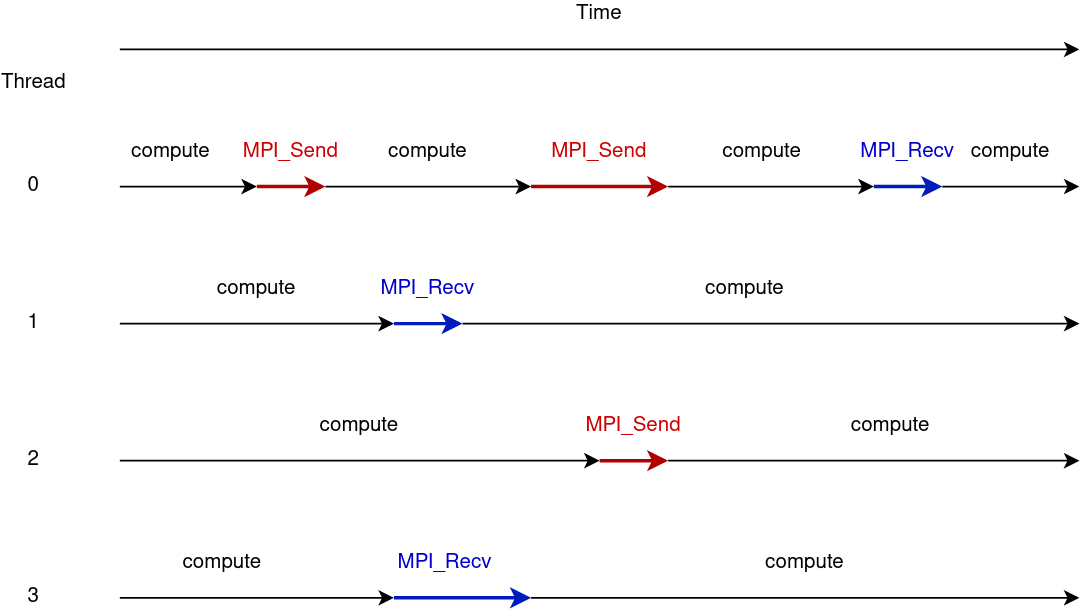
\includegraphics[width=10cm, height=6cm]{./other_images/mpi_multiple.png}
    \caption{\label{fig:mpi_multiple} Visualization of MPI Multiple mode. Each OMP 
    thread can make MPI calls.}
\end{figure}

The idea behind this, is to avoid the creation of a parallel region every time 
we iterate over the time steps and have multiple threads make MPI calls contemporarily. 
To do this, we need to initialize MPI slightly differently, as shown below:

\begin{lstlisting}[language=C++]
int provided_thread_level;
MPI_Init_thread(&argc, &argv, MPI_THREAD_MULTIPLE, &provided_thread_level);
if(provided_thread_level<MPI_THREAD_MULTIPLE)
{
    printf("Can't do thread multiple mode... Aborting");
    MPI_Finalize();
}
\end{lstlisting}

Then, the for loop over the evolution time steps looks like this:

\begin{lstlisting}[language=C++]
// single parallel region
#pragma omp parallel
for(unsigned long int t = 1; t < n+1; ++t)
{

    // multiple threads make MPI calls

    // nowait eliminates barrier at the end
    #pragma omp single nowait
    MPI_Irecv(data_prev, cols, MPI_CHAR, prev, next_tag, MPI_COMM_WORLD, &prev_recv_request);

    #pragma omp single nowait
    MPI_Irecv(data_prev + my_rows_x_cols_p_cols, cols, MPI_CHAR, next, prev_tag, MPI_COMM_WORLD, &next_recv_request);

    #pragma omp single nowait
    MPI_Isend(data_prev + cols, cols, MPI_CHAR, prev, prev_tag, MPI_COMM_WORLD, &prev_send_request);

    #pragma omp single nowait
    MPI_Isend(data_prev + my_rows_x_cols, cols, MPI_CHAR, next, next_tag, MPI_COMM_WORLD, &next_send_request);

    // remaining threads in the meantime start to work on internal part 
    // of grid. We need to keep the implied barrier at the end of the for loop 
    // because the next operation of waiting can only happen if send and recv 
    // have been posted
    #pragma omp for schedule(dynamic, chunk)
    for(unsigned long int cell = 2*cols; cell< my_rows_x_cols; ++cell)
    {
            unsigned long int i = cell/cols;
            unsigned long int j = cell - i*cols;
            upgrade_cell_static(data_prev, data, i, j);
    }//barrier. Needed, otherwise, if threads havent finished posting 
     //send and receive, the next operation will be an error.

     // we wait until we receive halo rows
    #pragma omp single
    {
        MPI_Wait(&prev_recv_request, MPI_STATUS_IGNORE);
        MPI_Wait(&next_recv_request, MPI_STATUS_IGNORE);
        MPI_Request_free(&prev_send_request);
        MPI_Request_free(&next_send_request);
    } //barrier needed because we need to get halo cells to process 
      //next rows. Now we can process the first and last row.

    // threads can split row 1 further. Note the nowait clause.
    #pragma omp for schedule(dynamic, small_chunk) nowait
    for(unsigned long int col=0; col<cols; ++col)
    {
        upgrade_cell_static(data_prev, data, 1, col);
    }

    // once done with row above, threads will start immediately 
    // on the last row.
    #pragma omp for schedule(dynamic, small_chunk)
    for(unsigned long int col=0; col<cols*(my_rows>1); ++col)
    {
        upgrade_cell_static(data_prev, data, my_rows, col);
    }// barrier since I need to wait for all threads to finish before 
     // saving and swapping

    // implied barrier at the end to finish saving and swapping
    #pragma omp single
    {
        ++save_counter;
        if(s>0 && save_counter == s && t<100000)
        {
            sprintf(snapshot_name, "snapshot_%05ld", t);
            save_grid(snapshot_name, MPI_COMM_WORLD, rank, header, header_size, my_total_file_offset, data, my_rows, cols);
            save_counter = 0;
        }

        tmp_data = data;
        data = data_prev;
        data_prev = tmp_data;
        tmp_data = NULL;
    }// barrier
} // barrier
\end{lstlisting}

The snippet is well commented and explained. However, we briefly touch on some 
important points. Since we create a single parallel region, we will need to 
be careful with the synchronization. For example, after the for loop on the 
internal cells, we have an implied barrier that we cannot elimiate otherwise the 
wait operation may give an error (if execute before the recv has been posted).

There is another implied barrier after the wait clauses, since we need to wait 
to receive the halo rows before processing the first and last rows.

There is another implied barrier after we process the last row, since 
we need to process the whole grid before possibly saving. Finally, there is another 
implied barrier before going on to the next step of the evolution, otherwise the 
data regions may not have been swapped.

In total, we have four implied barriers, which, as we will see later, kills  
performance.

\subsection{OMP Integration - Hybrid V2}

The second versions tries to be as simple as possible. 

During our development path for this project, we wrote a serial version, several
pure OMP versions, and pure MPI version before writing the hybrid version. 
This is one of the first implementations we had attempted but discared for being 
too simple. Finally, we decided to come back to it because of its simplicity. 

The idea is to add simply put a pragma parallel for construct on top of the 
first for loop over the rows. In this way, each thread updates a subset of the 
rows - similar to how each MPI process gets its part of the grid.

The code is shown below:

\begin{lstlisting}[language=C++]
for(unsigned long int t = 1; t < n+1; ++t)
{

    MPI_Isend(data_prev + cols, cols, MPI_CHAR, prev, prev_tag, MPI_COMM_WORLD, &prev_send_request);

    MPI_Isend(data_prev + my_rows_x_cols, cols, MPI_CHAR, next, next_tag, MPI_COMM_WORLD, &next_send_request);

    MPI_Irecv(data_prev, cols, MPI_CHAR, prev, next_tag, MPI_COMM_WORLD, &prev_recv_request);

    MPI_Irecv(data_prev + my_rows_x_cols_p_cols, cols, MPI_CHAR, next, prev_tag, MPI_COMM_WORLD, &next_recv_request);

    #pragma omp parallel for schedule(dynamic, chunk)
    for(unsigned long int row = 2; row < my_rows; ++row)
    {
        for(unsigned long int col = 0; col < cols; ++col)
        {
            upgrade_cell_static(data_prev, data, row, col);
        }
    }

    MPI_Wait(&prev_recv_request, MPI_STATUS_IGNORE);
    MPI_Wait(&next_recv_request, MPI_STATUS_IGNORE);
    MPI_Request_free(&prev_send_request);
    MPI_Request_free(&next_send_request);

    for(unsigned long int col=0; col<cols; ++col)
    {
        upgrade_cell_static(data_prev, data, 1, col);
    }

    for(unsigned long int col=0; col<cols*(my_rows>1); ++col)
    {
        upgrade_cell_static(data_prev, data, my_rows, col);
    }

    ++save_counter;
    if(s>0 && save_counter == s && t<100000)
    {
        sprintf(snapshot_name, "snapshot_%05ld", t);
        save_grid(snapshot_name, MPI_COMM_WORLD, rank, header, header_size, my_total_file_offset, data, my_rows, cols);
        save_counter = 0;
    }

    tmp_data = data;
    data = data_prev;
    data_prev = tmp_data;
    tmp_data = NULL;
}
\end{lstlisting}

The code is virtually the same, so we briefly comment the most significant 
details. First, we create a parallel region at \textit{each} time step. 
Second, we only paralellize the outer for loop over the rows, which means that 
in the extreme case where we have 1 row per process, the multhreading wont do 
anything. However, this is a very unlikely scenario, since to do this, we need 
as many processes and rows, and in this case, the issue will be with communication 
rather than lack of multithreading.

Finally, we explain \textit{why} we initially got rid of this version, and then 
came back to it, calling it \texttt{V2}.

As mentioned above, we first developed some serial and pure OMP versions before 
doing the hybrid version. Originally one of our main preoccupations was that this 
version introduced a lot of overhead due to the creation of the parallel regions 
each time. This eventually led to putting the pragma construct outside of the 
for loop over the time steps and developing the mpi multiple mode. 

Furthermore, another preoccupation, was that in the case of one row per process, 
this version would not paralellize using OMP. It seemed much more practical and 
elegant that the OMP would \textit{always} help by splitting up whatever each 
process had to do. 

However, we realized that by putting the parallel region outside, we needed to 
insert more barriers. Running some quick tests on pure OMP versions on our machine 
also didn't seem to yield substantial differences.

Finally, we decided to test it out, just to see how it would perform.

\subsection{Software Stack - Running the code}
On Orfeo, we always used the Open MPI module compiled against gcc version 12.2.1. 

To compile the code, we provided a Makefile, which automatically compiles the 
source code. We used as many error flags as possible, such as \-Wall, \-Werror, and 
\-Wextra. Finally, to optimize as much as possible we compiled with \-O3 and 
\-march\=native. 

The binaries for THIN nodes and for EPYC nodes can be found in the aptly named  
folders.

To run the code we have the following options:

\begin{lstlisting}[language=bash]
$mpirun [mpi_opt] conway_hybrid_pgm.out -i -f fname -k K 
$mpirun [mpi_opt] conway_hybrid_pgm.out -r -f fname -n N -s S -e E
\end{lstlisting}
The first option is used to initialize and save a random playground of size 
$k \times k$ with name \texttt{fname}.
The second option loads a grid named \texttt{fname} and evolves it for N 
timesteps, saving every S steps, with modality E. For the modality, 0 stands 
for ordered evolution, while 1 stands for static.

\subsection{Miscellaneous}

We briefly discuss some additional miscellaneous details. 

To time the code, we used \texttt{MPI\_Wtime()}, along with a reduction 
operation to compute the mean among all processes. This was inserted right 
before and right after the for loop over the time steps to avoid including the 
serial overhead of setting up everything for the evolution. 

To check for correctness of our code, we created a bash script called 
\texttt{check.sh}. This bash script runs all the implementations we have created 
with two famous examples, the glider gun and the snark loop, and compares the 
snapshots created at the end among the different versions. 

Since we have created a very simple serial version which we are sure is correct, 
this gives us some security in the correctness of the other implementations. 
However, if one wanted to be more thorough, it would be better to create various 
unit tests for each of the rule of conway and test against these.

Lastly, we briegly talk about the contents of our folder. We have many implementations.
Some of these were developed along the way to test some personal curiosities and 
to better guide us in the development of our final hybrid code. 

In particular, we have a serial version we used mainly to be sure of the correctness 
of our results. We have three pure OMP implementations, which we used to test 
different ways to parallelize using OMP and to see some differences with respect 
to where we place the parallel regions and other things. Finally, we also have a 
pure MPI version which we initially implemented to begin thinking in parallel and 
we used as a base for the hybrid code. 

In the \texttt{patterns\_pgm} directory we find the PGM files for the gosper glider gun and 
for the snark loop. Furthermore, in the \texttt{pattern\_gifs} we find small videos 
that we produced on our local machine to visualize the results of our evolution 
using the ffmpeg utility. The snippet below shows how to do this: 

\begin{lstlisting}[language=bash]
    $mpirun -np 8 conway_hybrid_pgm.v2.out -r -f snark_loop.pgm -n 400 -s 1 -e 1 
    $ffmpeg -framerate 100 -f image2 -vcodec pgm -i snapshot_%05d my_gif.mkv
    $mpv my_gif.mkv
\end{lstlisting}

\section{Bonus - Algorithm 2}
\section{Results and Discussion}

As mentioned in the introduction, we analyzed different scenarios. 
Each of these was repeated on both EPYC and THIN nodes when possible. 
However, since THIN nodes were generally less occupied, most of our 
results were taken for this architecture. 

\subsection{Strong OMP Scalability}

In this section, we use a single THIN of EPYC node, and fix the number of MPI 
tasks to 2, pinning each to one socket. Then, we slowly increased the 
number of OMP threads by changing the \texttt{OMP\_NUM\_THREADS} environment 
variable. This was done until we saturated each socket, i.e. 12 threads for THIN 
and 64 threads for EPYC. We used a randomly initialized grid with size fixed to 
$10k \times 10k$. We used 200 evolution steps and saved only at the end. 
We used \texttt{OMP\_PLACES=cores} and \texttt{OMP\_PROC\_BIND=close}.

This corresponds to using the following setup:  

\begin{lstlisting}[language=bash]
$export OMP_NUM_THREADS={NUM}
$export OMP_PLACES=cores
$export OMP_PROC_BIND=close
$mpirun --map-by socket -np 2 conway_hybrid_pgm.v2.c -r -f grid_010k -n 200 -s 0 -e 1
\end{lstlisting}

We repeated the measurements 10 times to obtain a statistical average and standard 
deviation. Below are the results for THIN nodes:

\begin{figure}[H]
\centering
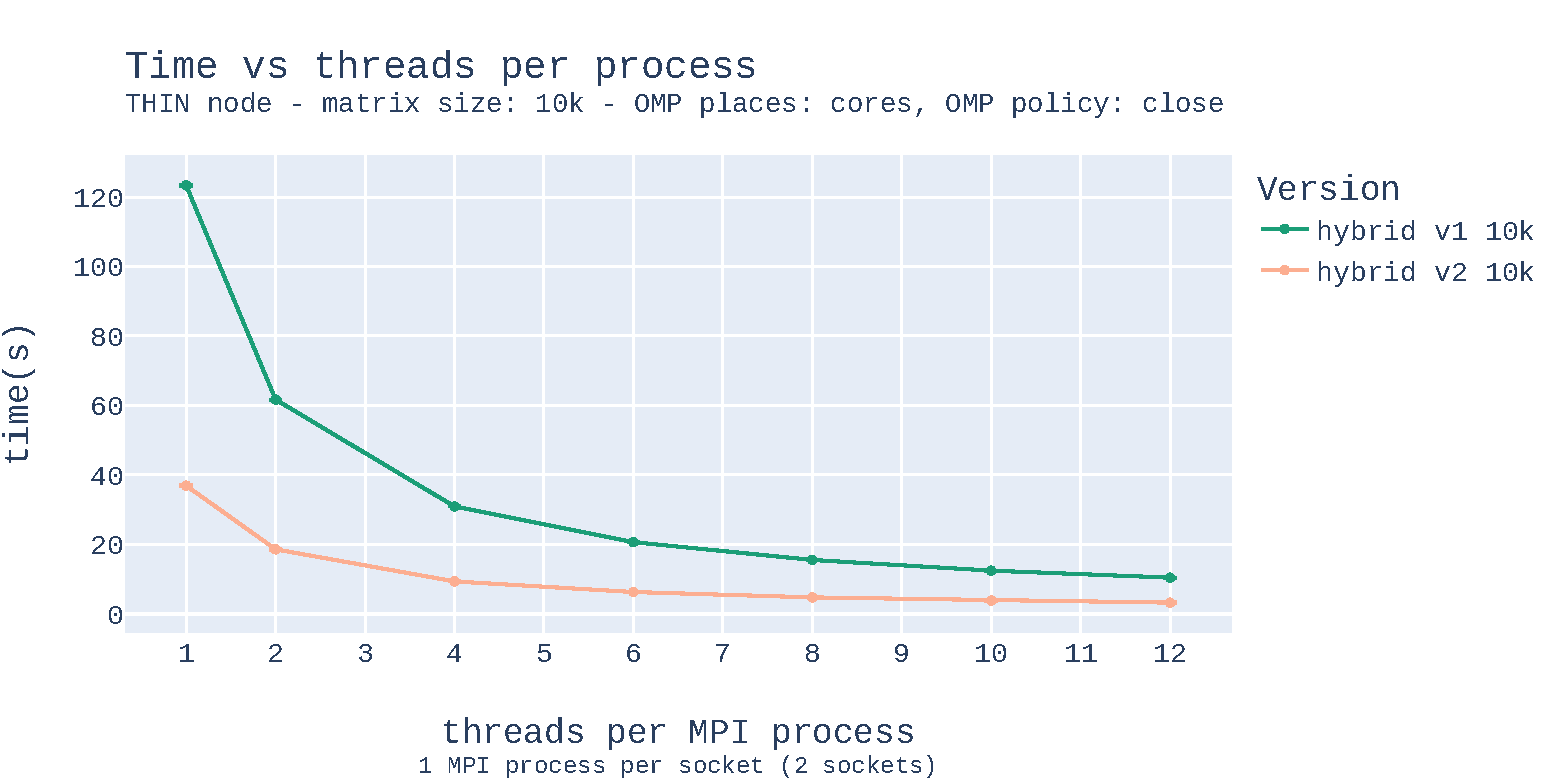
\includegraphics[width=14cm, height=7cm]{./images/strong_OMP_thin_hybrid_grid_010k.pdf}
\caption{\label{fig:strongomp10kspeedupthin} Time for THIN nodes with a 
random grid of size $10k \times 10k$. V1 takes almost three times as long as V2.}
\end{figure}

As we can see, version 1 (V1) takes almost three times the amount of time of 
version 2 (V2). This confirms our initial supposition that all the barriers 
that were introduced in V1 killed the performance. 

We also decided to test our implementation on bigger matrices. However, due to 
limitations on job times, we limited our study to V2 for bigger matrices. 
We repeated the approach for matrices of size $20k\times 20k$ and $40k\times 40k$. 
However, this time, the sample size for $20k$ and $50k$ were 5 and 3, respectively.

Below we show the results: 

\begin{figure}[H]
\centering
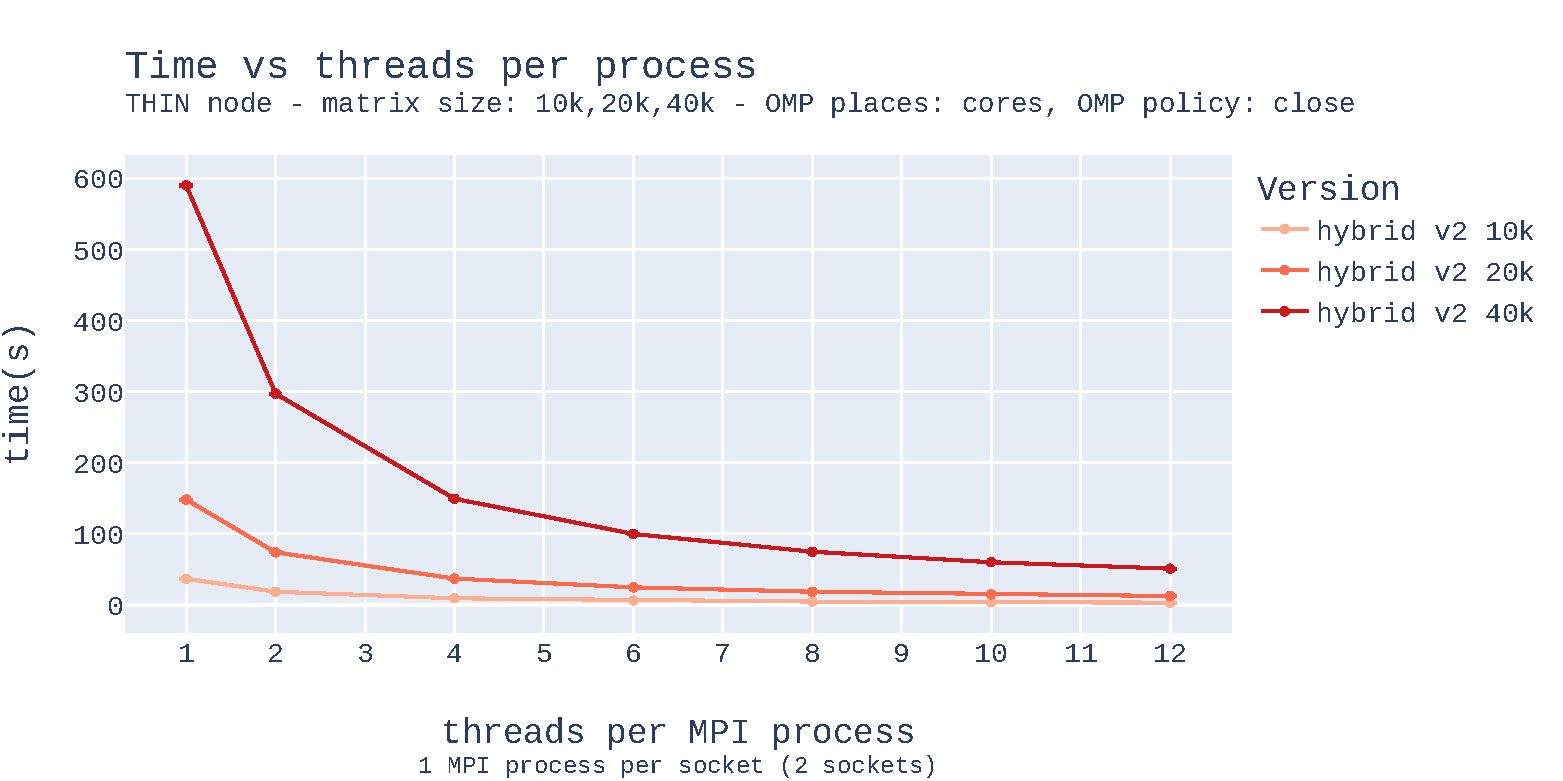
\includegraphics[width=14cm, height=7cm]{./images/strong_OMP_thin_hybrid_v2.pdf}
\caption{\label{fig:strongompv2thin} Time for THIN nodes for V2 with increasingly
bigger grids.}
\end{figure}

Below we show the speedup for all of these runs.

\begin{figure}[H]
\centering
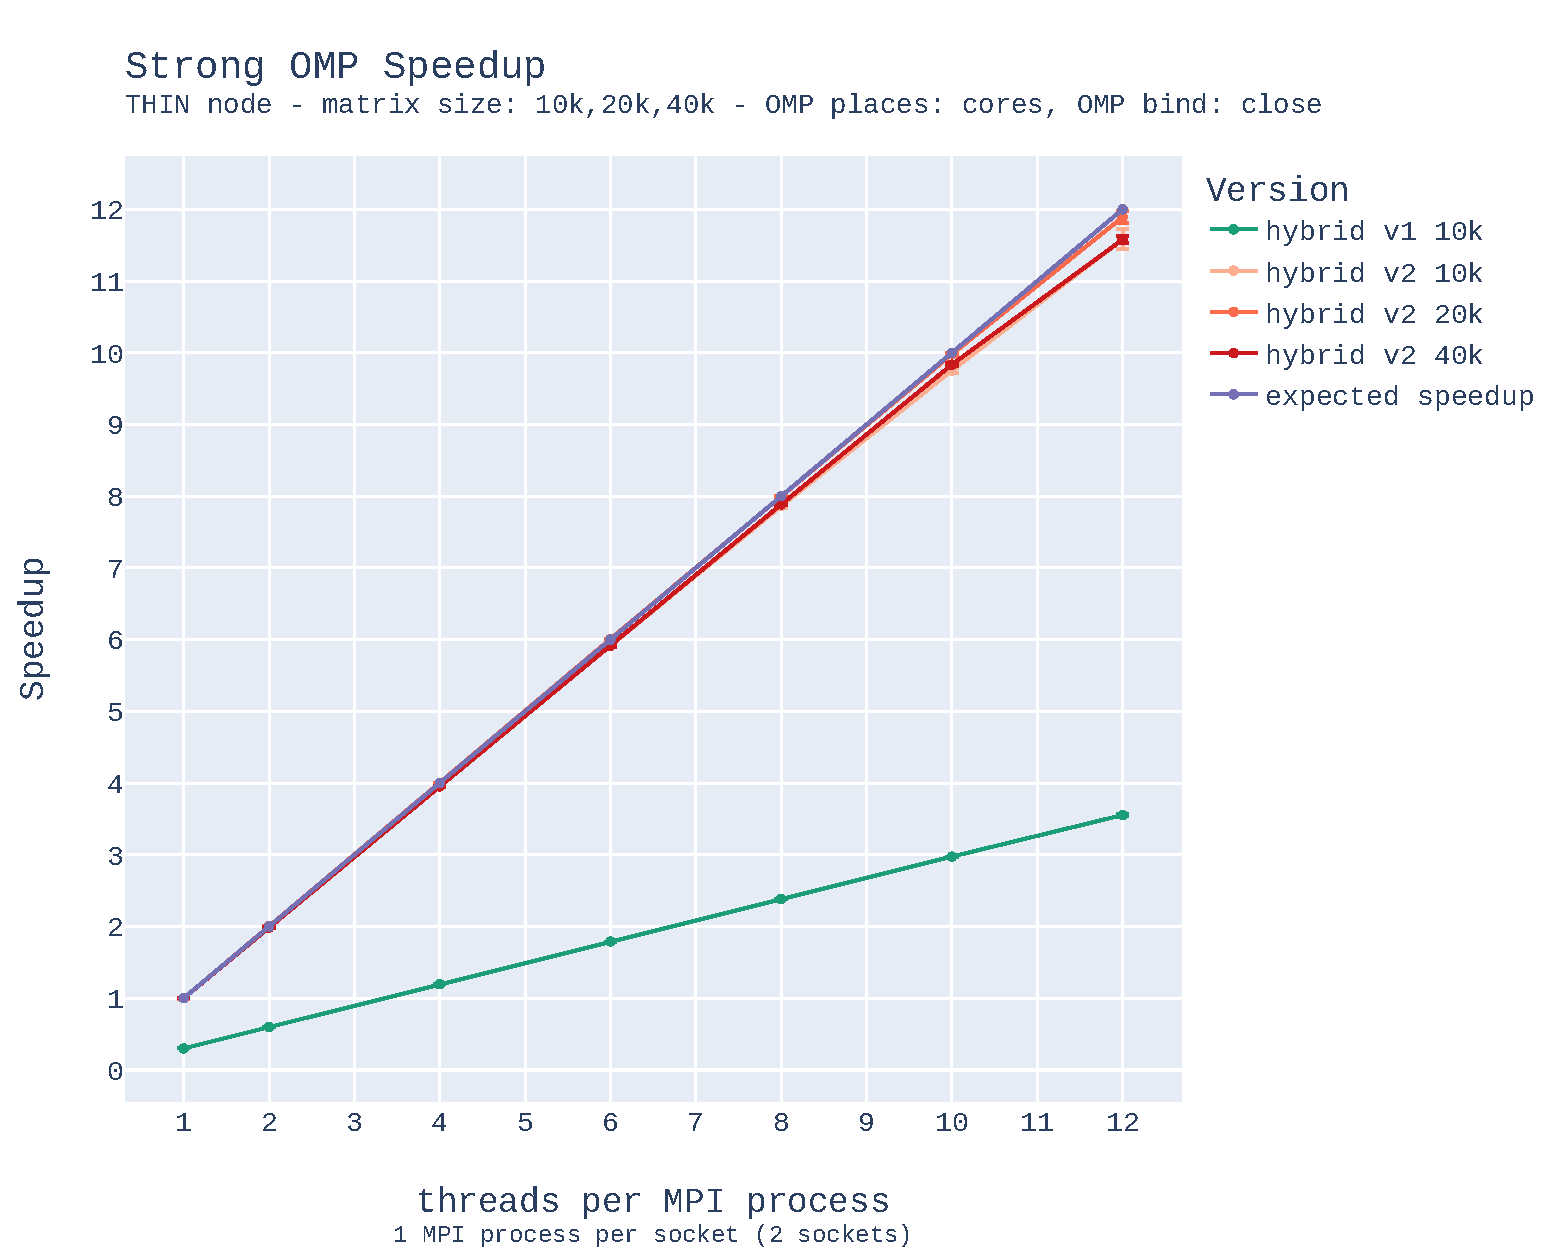
\includegraphics[width=10cm, height=8cm]{./images/strong_OMP_thin_hybrid_speedup.pdf}
\caption{\label{fig:strongompspeedupthin} Speedup for strong OMP scalability using 
increasingly bigger grid sizes for V2. As we can see, V1 scales poorly due to the 
barriers that were introduced. V1 scales very well, indicating that our code 
is well implemented.}
\end{figure}

As we can see, the speedup of version V2 is almost perfect. On the other hand, 
V1 is not scaling well. This is a final indicator that this implementation is not 
the best, due to the various barriers that were introduced. 

Furthermore, we see that V2 is able to scale well with increasingly bigger 
problem sizes that are 4 and 16 times as big as the original one. 
This is a good indicator that our code is written well, scalable, and efficient.   

Now we repeat the same experiments with an EPYC node.

In this we only ran experiments with the $10k$ grid. However, given the more 
complex architecture of EPYC nodes, we decided to experiment with the OMP policy.

Initially, we used \texttt{OMP\_PROC\_BIND=close} as we did for THIN. Then, we 
remembered that EPYC nodes have a particular architecture. They have two 
sockets, like THIN, however, inside each socket, they have 2 NUMA regions. 

Therefore, we hypothesized that using \texttt{OMP\_PROC\_BIND=spread} 
would give better results since each thread would intially be mapped, within the 
socket, into different NUMA regions and exploit the cache better.

Below we show the results for both hybrid versions, with both policies. We show 
both the time and the speedup.

\begin{figure}[H]
\centering
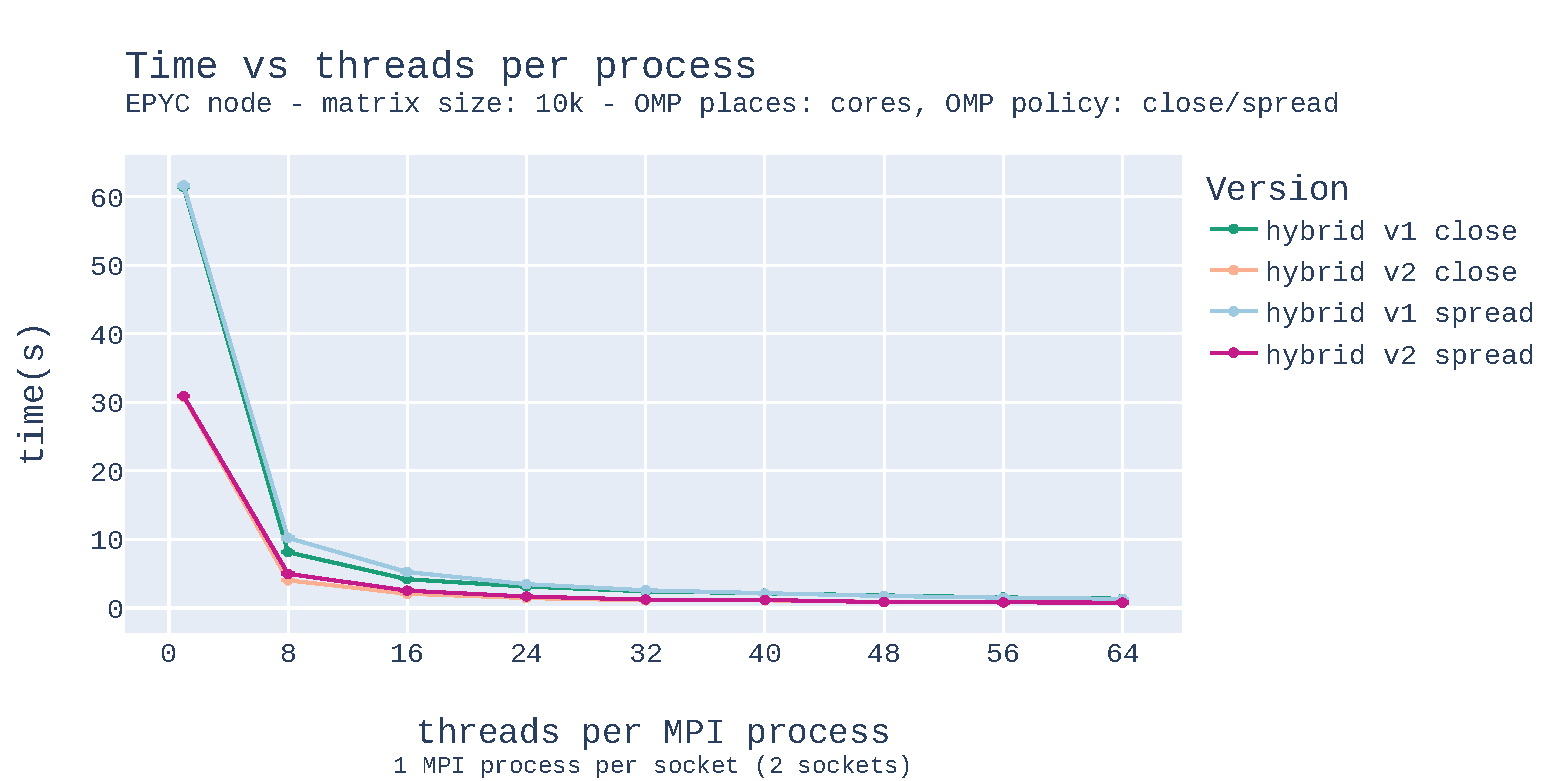
\includegraphics[width=14cm, height=7cm]{./images/strong_OMP_epyc_hybrid_grid_010k.pdf}
\caption{\label{fig:strongomp10kepyc} Time for EPYC nodes using a random grid of size 
$10k$ and both \texttt{OMP\_PROC\_BIND=close} and \texttt{OMP\_PROC\_BIND=spread}. 
Results for both V1 and V2 are shown.}
\end{figure}

\begin{figure}[H]
\centering
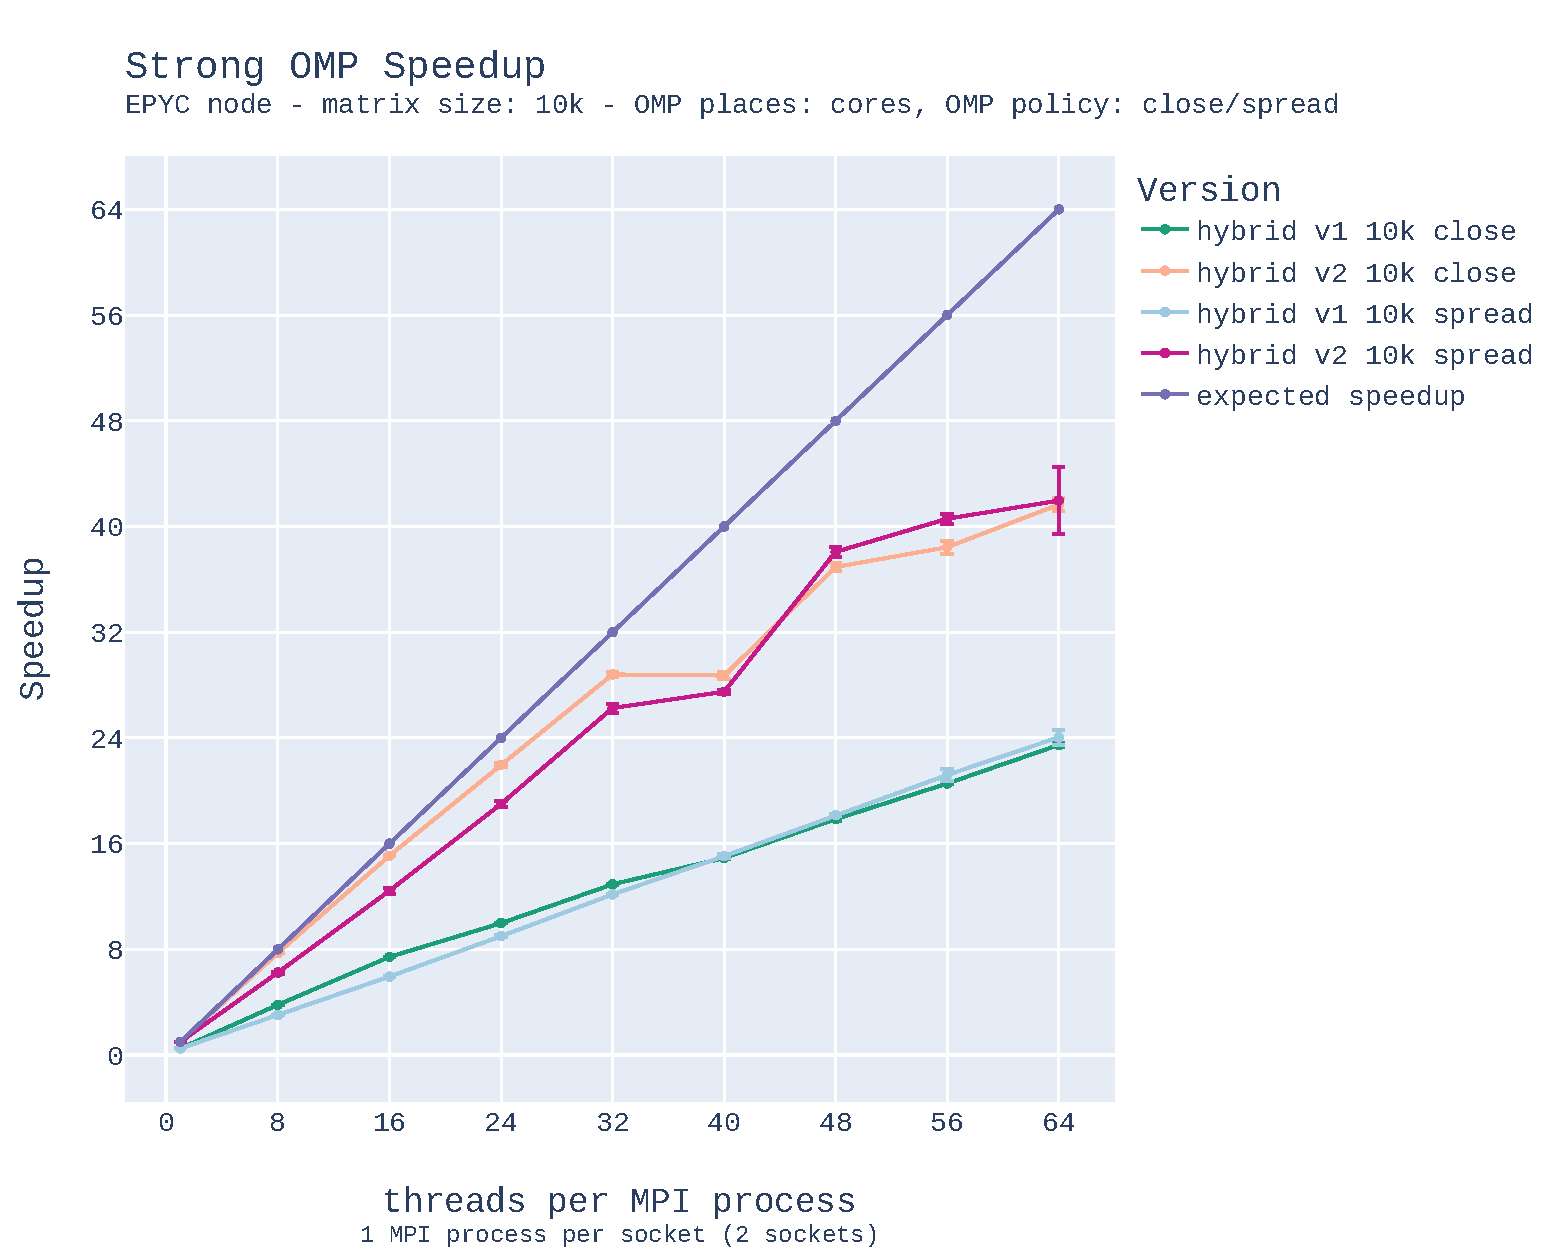
\includegraphics[width=10cm, height=8cm]{./images/strong_OMP_epyc_hybrid_grid_010k_speedup.pdf}
\caption{\label{fig:strongomp10kspeedupepyc} something}
\end{figure}

First, we notice that the OMP policy barely changes the results. This leads us 
to think that using different NUMA regions is not as beneficial as we thought. 
However, considering the results of the previous chapter, it may be the case 
that with much bigger matrix sizes, we may obtain some benefits.

Furthermore, once again, we see that V1 does not scale well, regardless of the 
OMP policy that we use. On the other hand, V2 seems to achieve scale well until 
we start to use half of each socket (32 threads per process). A possible explanation 
for this is that when we start to use more threads we begin to incur in more 
overhead for creation of the regions, management of the threads, and so on. 

However, when we use the full node, we still achieve $\sim 64\%$ of the theoretical 
speedup, which is not a terrible result.

It would be interesting to run the same experiments with much bigger grids, 
such as $50k \time 50k$.

\subsection{Strong MPI Scalability}

In this section, we fix the number of OMP threads per MPI process to 1, and we 
continuously increase the number of MPI tasks across the most nodes we can get 
for each architecture. 

For these experiments, we wanted to use much bigger grids to test the limits 
of our implementation. However, given the poor results for V1, we 
decided to test only V2. This choice was also made for practical time 
constraints as the V1 version took too long to execute on these larger grids. 

On THIN, we used 3 nodes and grids of sizes $50k$, $70k$, and $100k$. The last 
one is approximately 10 GBytes of data. On EPYC, we used 4 nodes and used the 
same grid sizes, to have a comparison.

Results were taken 5 times to get an average.

Below we show the results for THIN:

\begin{figure}[H]
\centering
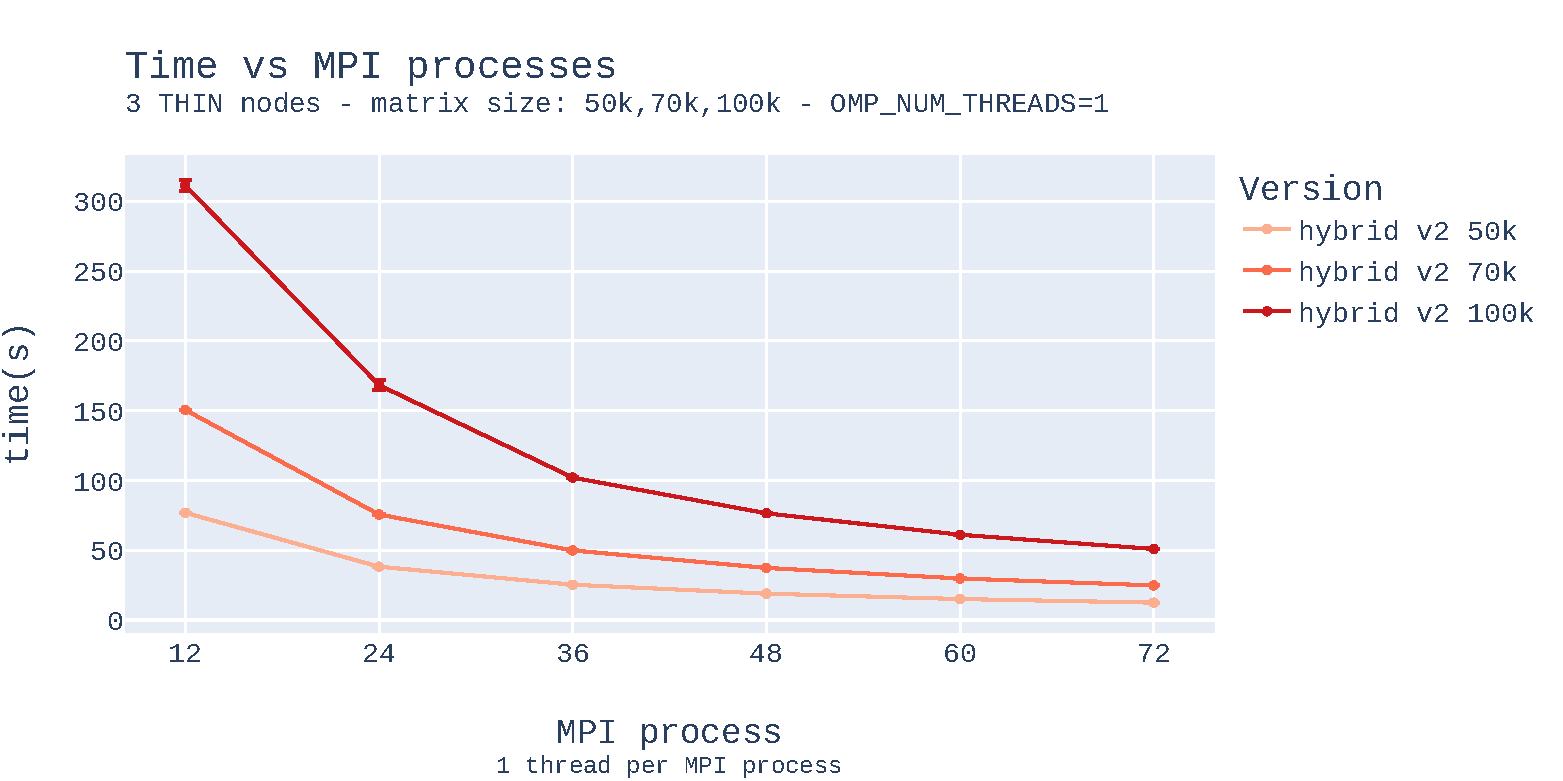
\includegraphics[width=14cm, height=7cm]{./images/strong_MPI_thin_hybrid.pdf}
\caption{\label{fig:strongmpithinhybrid} somethng}
\end{figure}

\begin{figure}[H]
\centering
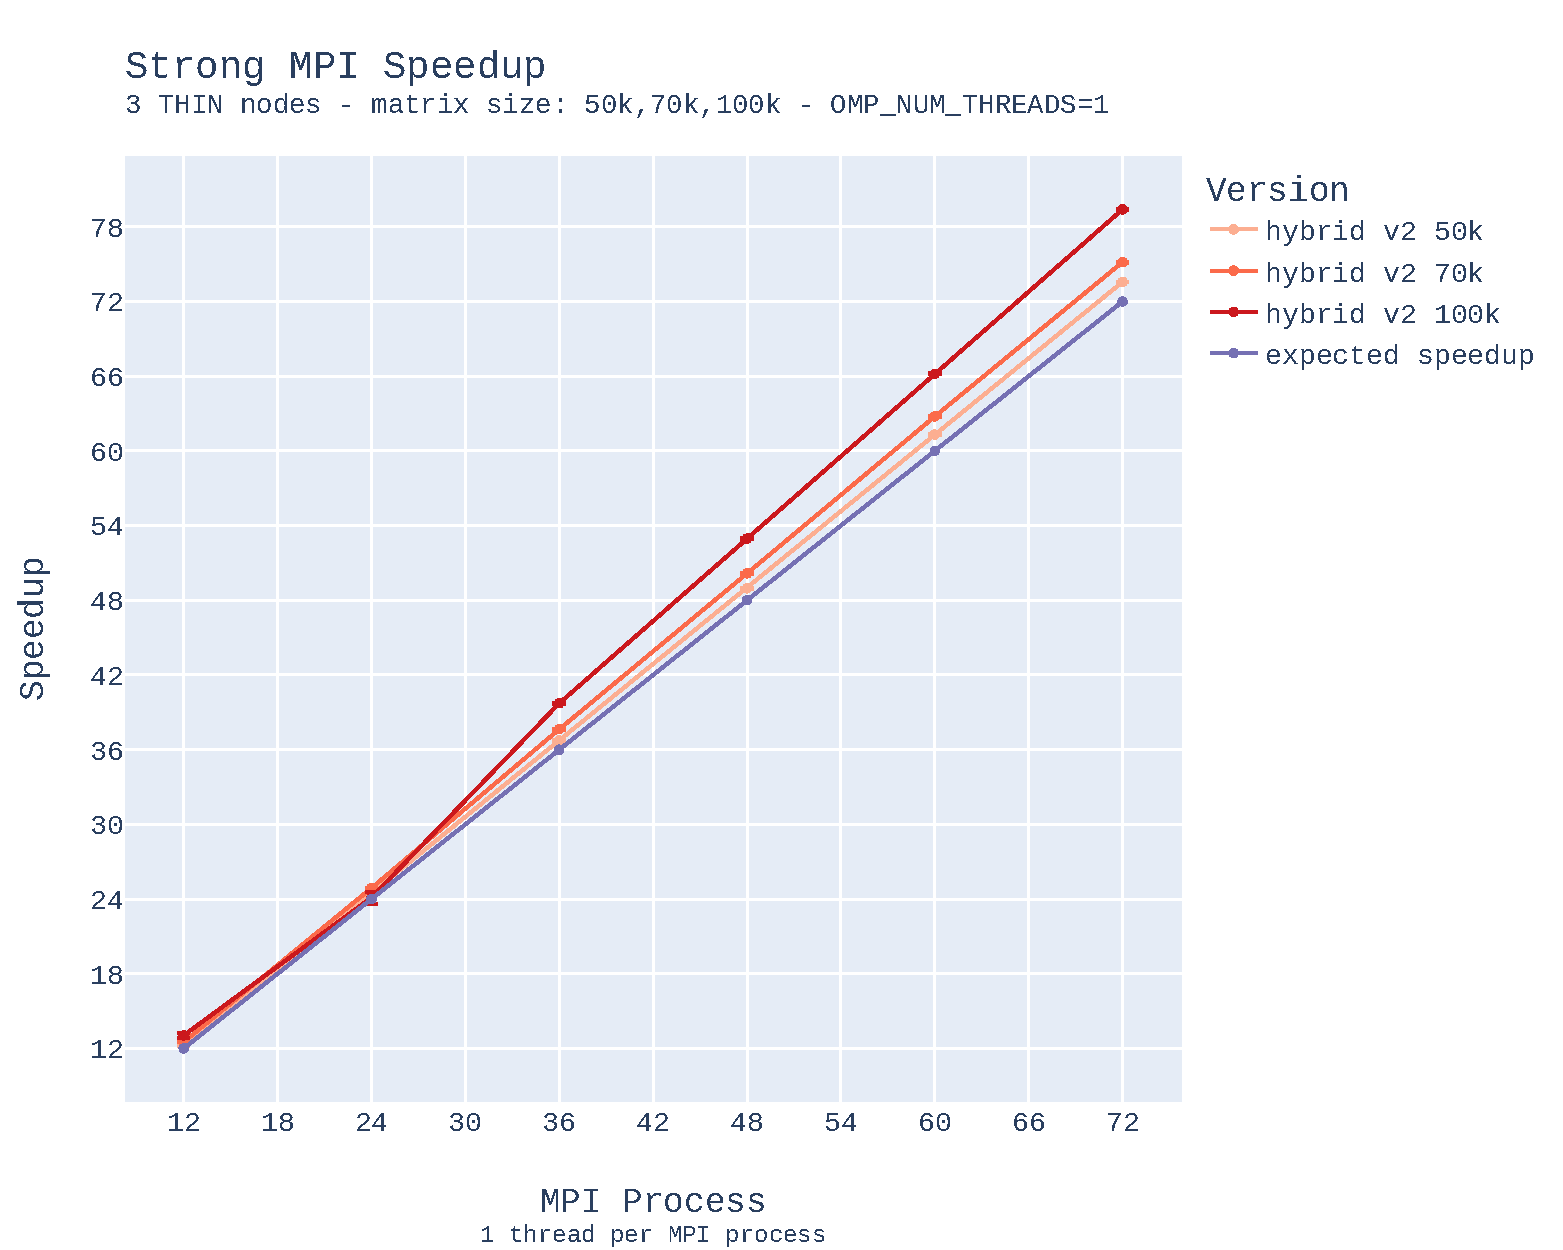
\includegraphics[width=10cm, height=8cm]{./images/strong_MPI_thin_hybrid_speedup.pdf}
\caption{\label{fig:strongmpithinhybridspeedup} somethng}
\end{figure}

As we can see, ... 

Now, we show the results for EPYC nodes.

\begin{figure}[H]
\centering
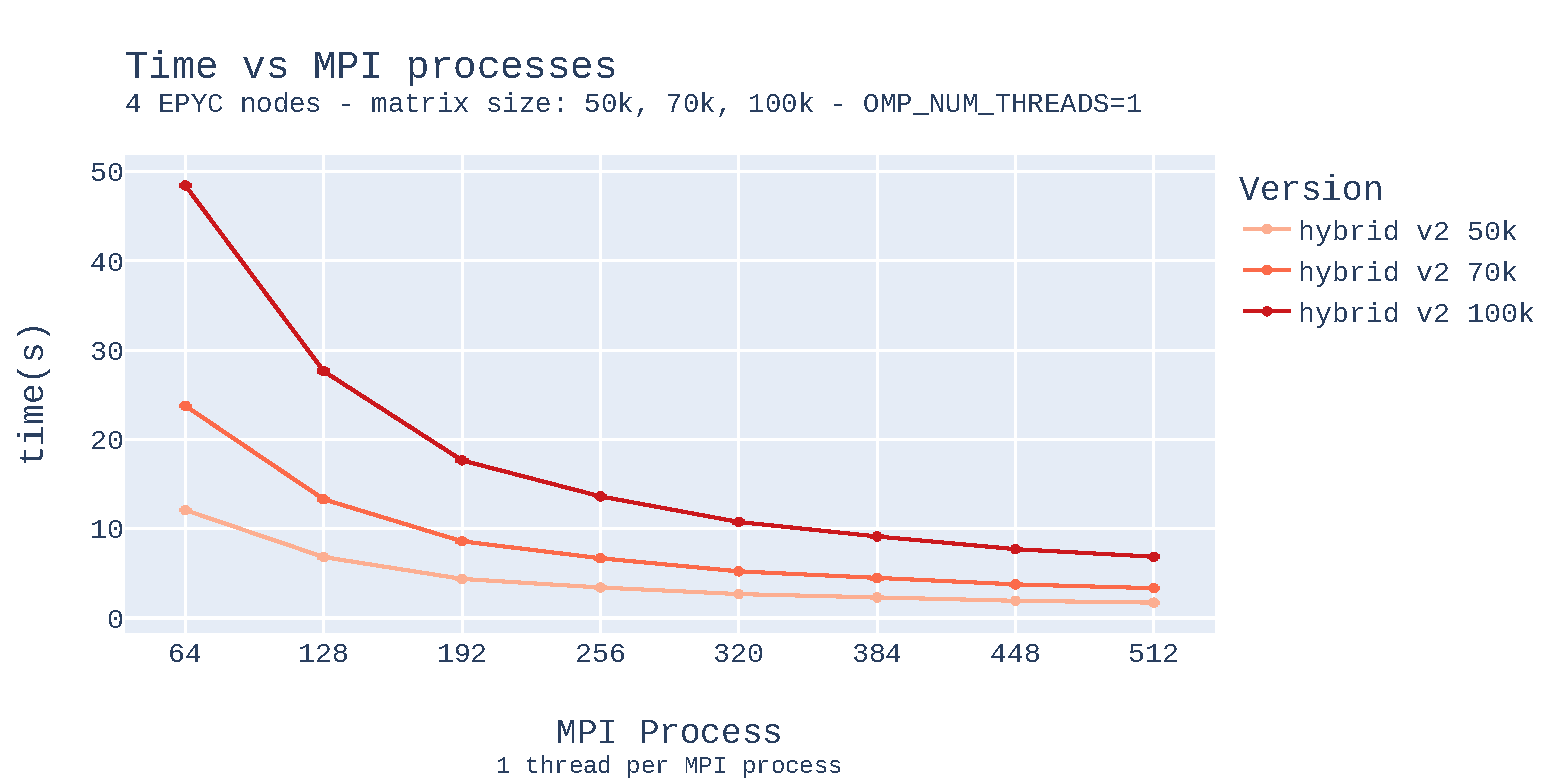
\includegraphics[width=14cm, height=7cm]{./images/strong_MPI_epyc_hybrid_grid_100k.pdf}
\caption{\label{fig:strongmpiepychybrid} somethng}
\end{figure}

\begin{figure}[H]
\centering
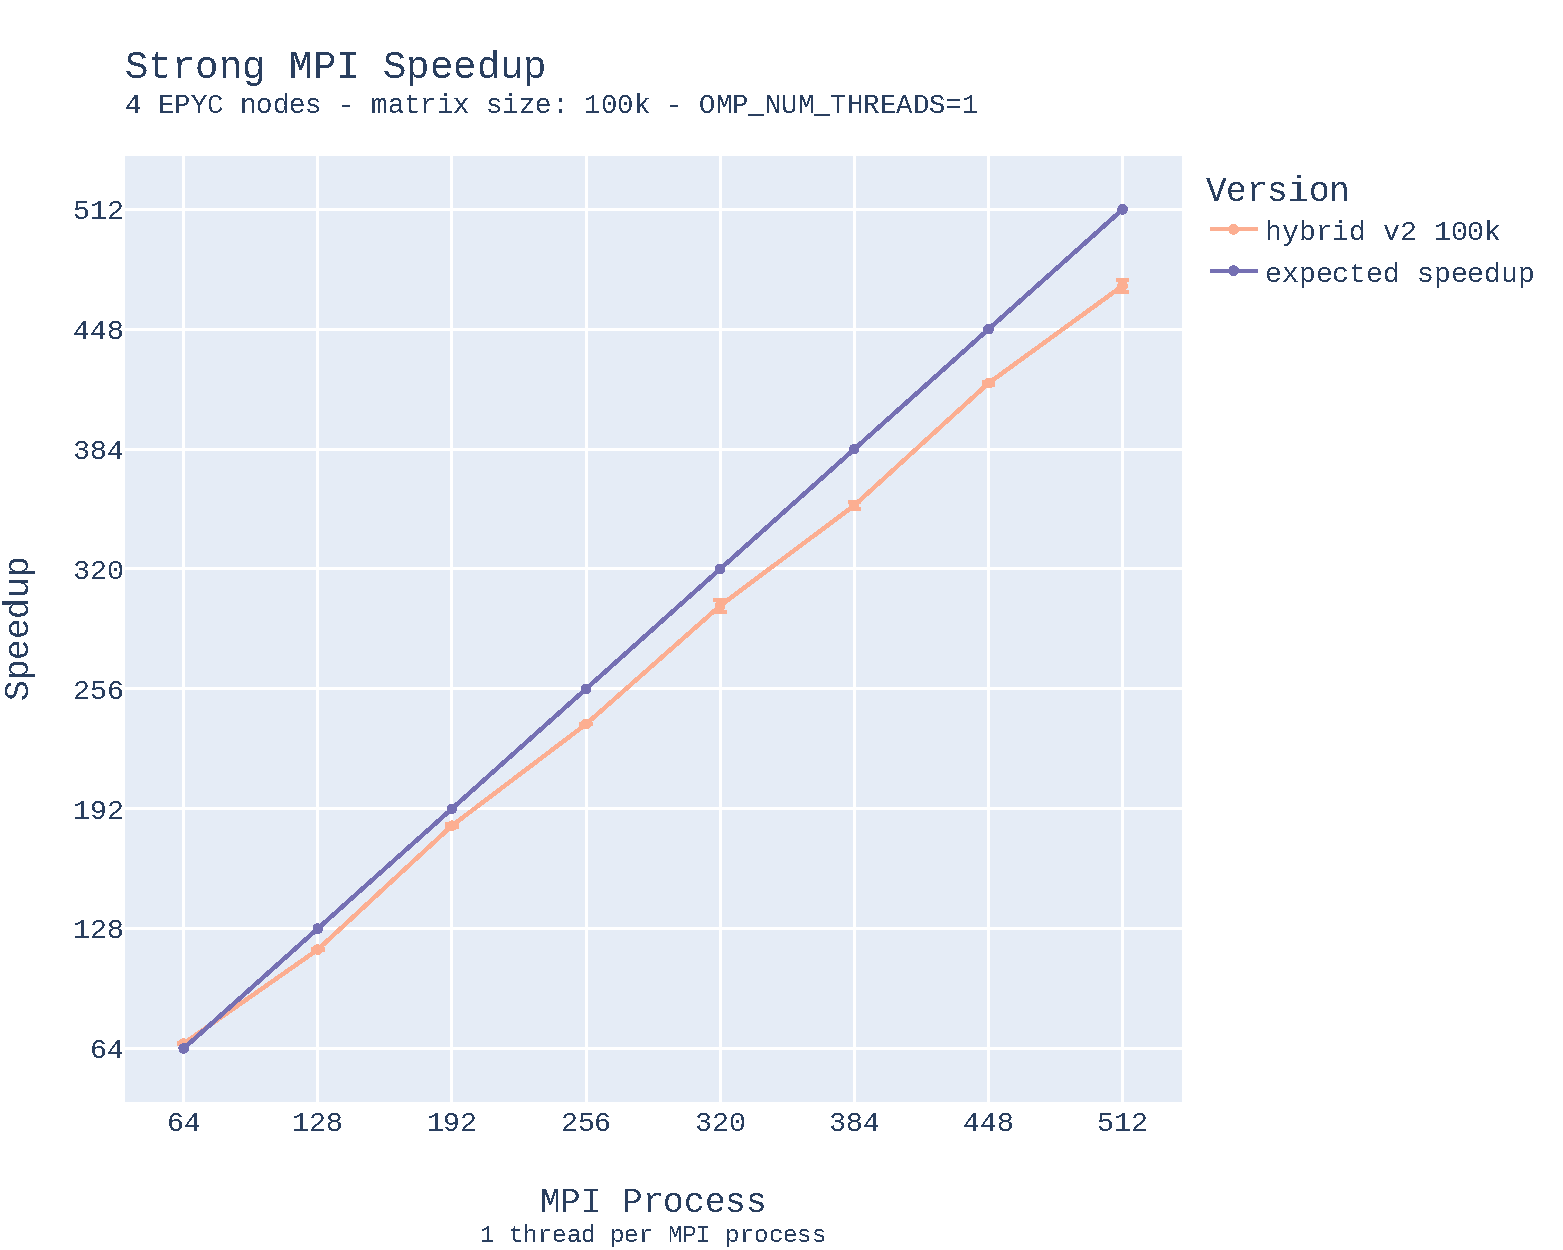
\includegraphics[width=10cm, height=8cm]{./images/strong_MPI_epyc_hybrid_grid_100k_speedup.pdf}
\caption{\label{fig:strongmpiepychybridspeedup} somethng}
\end{figure}

\subsection{Weak MPI Scalability}

In this section, we fixed the number of OMP threads to completely saturate a 
socket, i.e 12 for THIN and 64 for EPYC. Then, we slowly increased the number 
of MPI tasks, pinning them to sockets, across as many nodes as possible. However, 
as we increased the number of MPI tasks, we also increased the grid size to 
keep the workload per MPI task the same. In other words, if we doubled the number 
of tasks, we had to double the workload. Below we show the dimensions we used and 
the workload per MPI task.

Below we show a table with the dimensions we used:

\begin{table}[H]
\centering
\begin{tabular}{|c|c|c|c|c|c|}
    \hline
    Size & MPI Tasks & Work per MPI task \\\hline
    10000 &    1     & $\frac{10000^2}{1}=1.00000\times 10^8$ \\
    14142 &    2     & $\frac{14142^2}{2}=0.99998\times 10^8$\\
    17320 &    3     & $\frac{17320^2}{3}=0.99994\times 10^8$ \\
    20000 &    4     & $\frac{20000^2}{4}=1.00000\times 10^8$\\
    22360 &    5     & $\frac{22360^2}{5}=0.99993\times 10^8$\\
    24494 &    6     & $\frac{24494^2}{6}=0.99992\times 10^8$\\
    26457 &    7     & $\frac{26457^2}{7}=0.99996\times 10^8$\\
    28284 &    8     & $\frac{28284^2}{8}=0.99998\times 10^8$\\ \hline
\end{tabular}
\caption{\label{tab:weak}}
\end{table}

For THIN nodes, we only used three nodes. Below we show the results for the 
weak efficiency:

\begin{figure}[H]
\centering
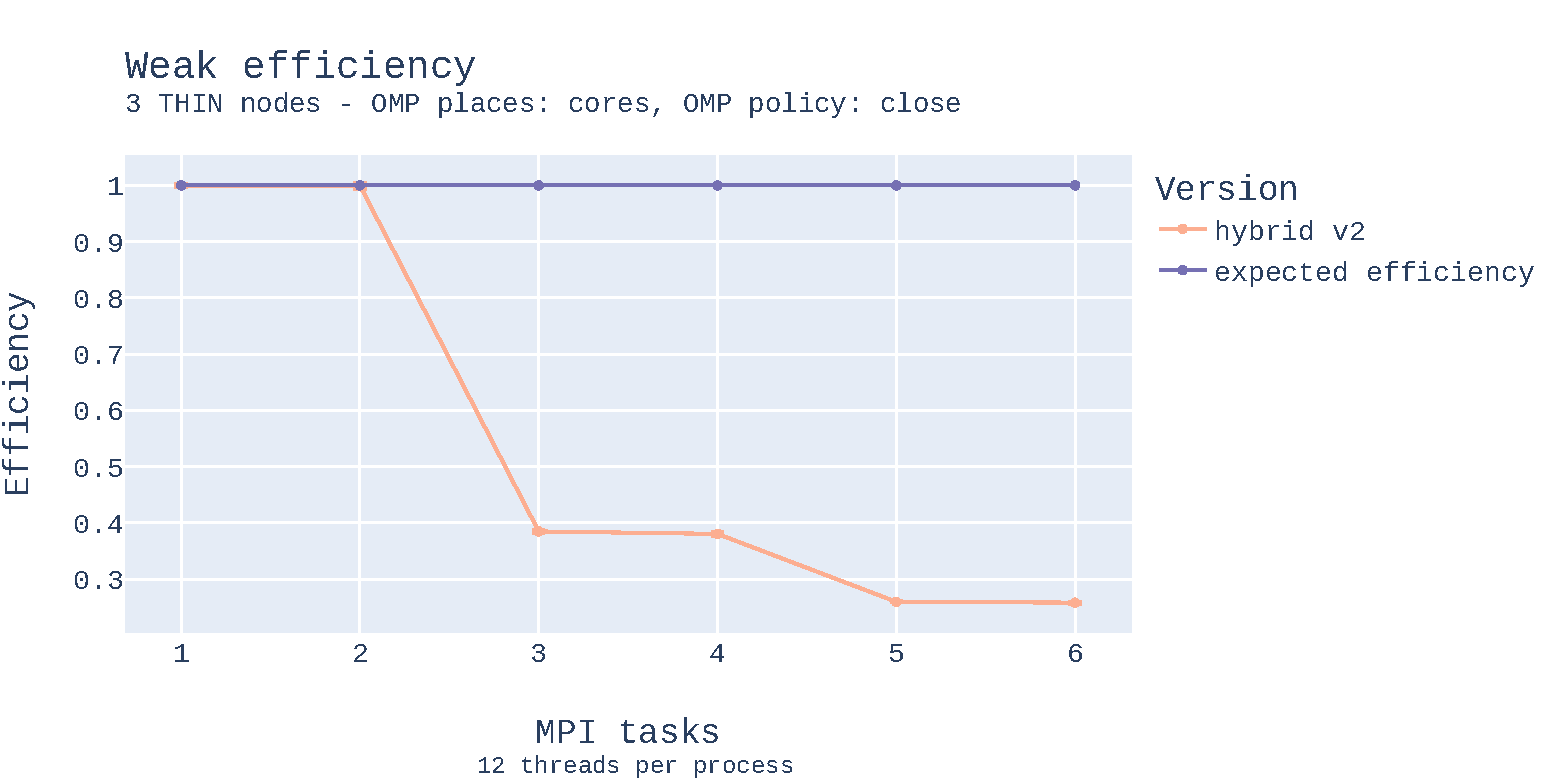
\includegraphics[width=14cm, height=7cm]{./images/weak_MPI_thin_hybrid.pdf}
\caption{\label{fig:weakmpithinhybrid} somethng}
\end{figure}

Now we show the results for EPYC nodes. In this case, we used four nodes in total.

\begin{figure}[H]
\centering
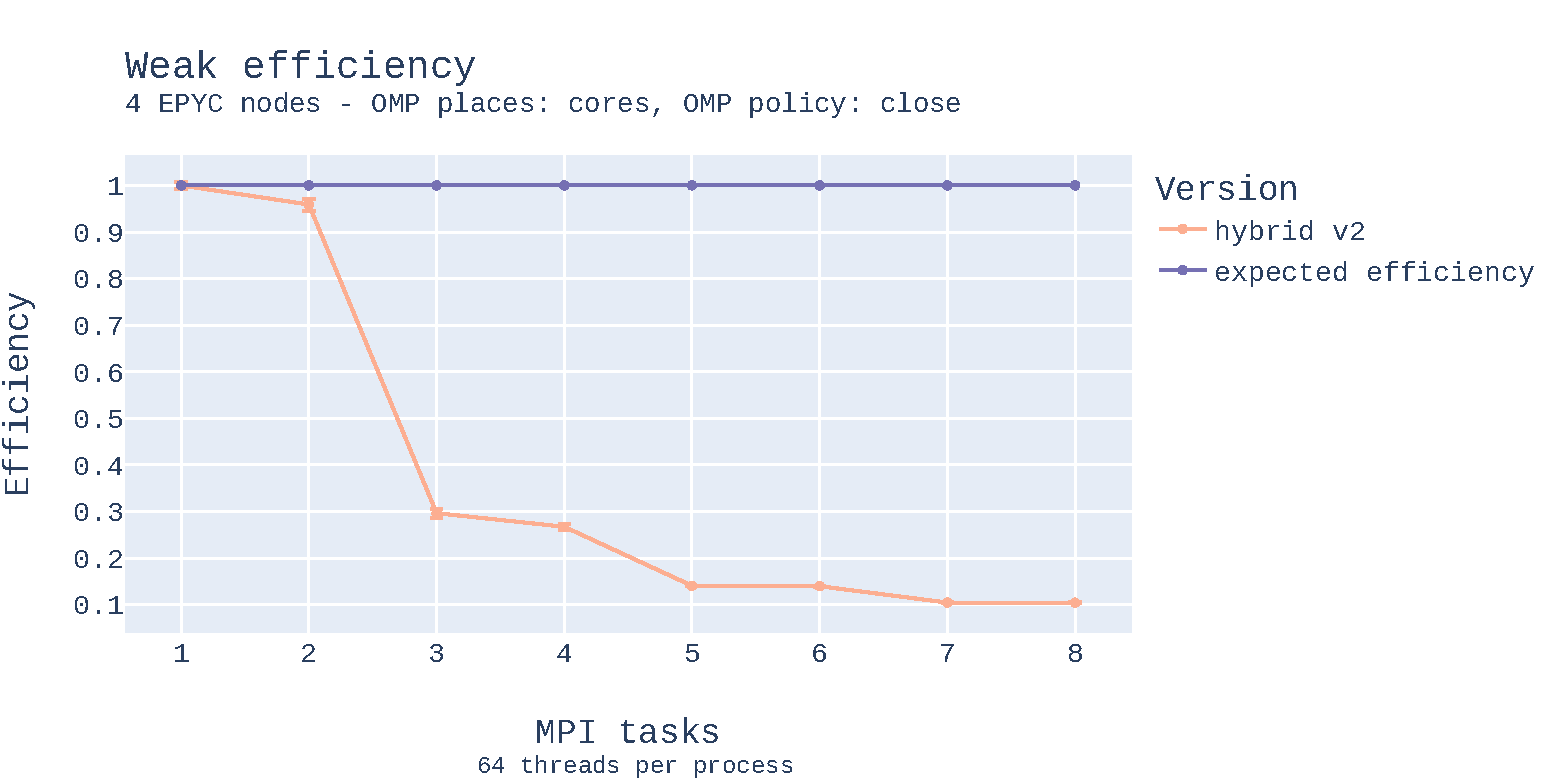
\includegraphics[width=14cm, height=7cm]{./images/weak_MPI_epyc_hybrid.pdf}
\caption{\label{fig:weakmpiepychybrid} somethng}
\end{figure}

\section{Conclusions}

\printbibliography

\end{document}
